\documentclass[a4paper,italian,11pt]{book}
\usepackage[utf8]{inputenc}
\usepackage{amsmath, amssymb, eucal, latexsym, multicol, amsthm, mathrsfs} 
\usepackage[toc,page]{appendix}
\usepackage{graphicx}
\usepackage{indentfirst}
\usepackage{float}
\usepackage{subfig}
\usepackage{booktabs}
\usepackage [font=small, format=hang, labelfont={sf, bf}]{caption}
\usepackage {subfig, wrapfig}
%\usepackage{arabtex}
\usepackage{verbatim}
\usepackage{color}
\renewcommand{\qedsymbol}{\rule{0.7em}{0.7em}}
\usepackage{listings}

\newcommand{\squeezeup}{\vspace{-0.5mm}}

\newcommand{\facciatabianca}{\newpage\shipout\null\stepcounter{page}}

%\makeatletter
%\def\remark@space@setup{\remark@preskip=0cm
%\remark@postskip=0cm}
%\makeatother
%\newtheoremstyle{newstyle}      
%   {0cm} %Aboveskip 

\newtheorem{theorem}{Theorem}

%\theoremstyle{newstyle}
% \theoremstyle{remark}
\newtheorem{remark}{Remark}

\theoremstyle{plain}
\newtheorem{definition}{Definition}

\theoremstyle{remark}
\newtheorem{identity}{Identity}

\theoremstyle{plain}
\newtheorem{proposition}{Proposition}
\newtheorem{lemma}{Lemma}

\newtheorem{corollary}{Corollary}

\title{Master thesis - second}
\author{Nicola Hu}
\date{September 2020}

\begin{document}


\begin{titlepage}
\begin{figure} [h]
\begin{center}
%\includegraphics[width=0.3 \textwidth]{logo.jpg}
\end{center}
\end{figure}
\begin{center}
{\Large Universit\`a degli Studi di Padova\\}
\vspace{8mm} 
{\Large Dipartimento di Matematica Tullio Levi Civita\\}
\vspace{8mm}
{\Large Courso di Laurea in Matematica\\}
\vspace{10mm}
{\LARGE \textbf{Titolo da decidere}\\}	

\vspace{30mm}
\end{center}
\par
\begin{minipage}[t]{0.5\textwidth}
{\Large \textit{Relatrice:}}
\end{minipage}
\hfill
\begin{minipage}[t]{0.5\textwidth} \raggedleft
{\Large \textit{Candidato: }}
\end{minipage}
\par
\vspace{1mm}
\begin{minipage}[t]{0.5\textwidth}
{\Large Prof. Callegaro Giorgia}
\end{minipage}
\hfill
\begin{minipage}[t]{0.5\textwidth} \raggedleft
{\Large Hu Nicola \\ \textit{Numero di matricola:} \\ 1217174\\}%\\ \vspace{1mm}
\end{minipage}
\vspace{25mm}
\begin{center}
{\large{
Academic Year 2020/2021}}
\end{center}
\end{titlepage}


\facciatabianca


\newpage
\tableofcontents
\pagestyle{headings}

\newpage

\section*{Notation}
\addcontentsline{toc}{chapter}{Notation}

\noindent 
$\bullet$ $\mathbb{C}$ are the complex numbers.
\\
\\
\noindent
$\bullet$ $\mathbb{R}_+$ are the positive real numbers.
\\
\\
\noindent
$\bullet$ $C^\alpha (\mathbb{R})$, for $\alpha \in (0,1]$, denotes the space of $\alpha$-Hölder continuous functions, defined below in Definiton \ref{def: holderContinuity}.
\\
\\
\noindent
$\bullet$ $AC([a,b])$ is the space of absolute continuous functions on $[a,b]$, where $-\infty \le a < b \le +\infty$. We remind that $f$ is absolutely continuous in $[a,b]$ if for any $\epsilon >0$, there exists $\delta >0$ s.t. for any finite set of $n$ disjoint intervals $[a_k,b_k]$ contained in $[a,b]$ satisfying $\sum_{k=1}^n (b_k-a_k) <\delta$, we have $\sum_{k=1}^n |f(a_k)-f(b_k)|<\epsilon$.
\\
\\
\noindent
$\bullet$ $AC^n([a,b])$, for $n$ positive integer and $-\infty \le a < b \le \infty$, is the space of functions $f$ with continuous derivatives up to the order $(n-1)$ on $(a,b)$ and with $f^{(n-1)}\in AC([a,b]).$
\\
\\
\noindent
$\bullet$ $\lfloor x \rfloor $ for $x \in \mathbb{R}$, denotes the largest integer smaller than $x$.
\\
\\
\noindent
$\bullet$ $\lceil x \rceil$ for $x \in \mathbb{R}$, denotes the smallest integer greather than $x$.
\\
\\
\noindent
$\bullet$ $\left\{x \right\}$ for $x \in \mathbb{R}$ is the fractional part of $x$, i.e. $\left\{ x \right\} = x-\lfloor x \rfloor$.
\\
\\
\noindent
$\bullet$ $\Gamma(x) = \int_0^{+\infty}s^{x-1}e^{-s}\, ds$, with $x>0$ is the Gamma function.
\\
\\
\noindent
$\bullet$ $B(x,y) = \int_0^1 s^{x-1}(1-s)^{y-1} \, ds$, with $x,y>0$ is the Beta function.

\chapter*{Introduction}
\addcontentsline{toc}{chapter}{Introduction}

The classical Heston model is the most famous stochastic volatility model describing the dynamics of $S$, the underlying asset price, and $V$, the variance process. It consists of the following stochastic differential equations:
\\
\\
\textbf{Classical Heston model.}
\begin{equation}
    \label{eq: classicalHeston}
    \begin{cases}
    dS_t = S_t \sqrt{V_t} dW_t, \\
    dV_t = \eta (m - V_t) dt +  \eta \zeta \sqrt{V_t} dB_t, \\
    S_0 = s_0 >0, \\
    V_0 = v_0 >0, \\            
    t \ge 0,
    \end{cases}
\end{equation}
\\
where $W$ and $B$ are two Brownian motions with correlation $\rho$ (i.e., \\
$Corr(dW_t,dB_t) = \frac{Cov(dW_t, dB_t)}{\sqrt{Var(dW_t)} \sqrt{ Var(dB_t)}} = \rho dt)$. 
% See 
% \href{https://quant.stackexchange.com/questions/25640/how-to-express-the-volatility-of-two-correlated-ito-processes-wt-1-wt-2-expre}{click here}
\\
In this model the volatility follows a standard Brownian motion.
\\

Despite its celebrity, it has been shown that this model does not represent accurately historical volatility time-series, as these happen to be rougher than what this model allows
(i.e., a standard Brownian motion). 
A ``roughening" of this version has been elaborated. This has been inspired by (see \cite{rosenbaum1}) the fractional Brownian motion (which is a generalization of the Brownian motion and allows for a rougher behaviour).
\\

A fractional Brownian motion $(W_t^H)_{t\ge 0}$ with Hurst index $H\in (0,1)$ can be expressed with the Mandelbrot-Van Ness integral representation (as we will see in more details later in subsection $1.1.2$):
\begin{equation}
    \label{eq: fBm Representation}
    W_t^H = \frac{1}{\Gamma(H+\frac{1}{2})}\int_{-\infty}^0 [(t-s)^{H-\frac{1}{2}}-(-s)^{H-\frac{1}{2}}]dZ_s + \frac{1}{\Gamma(H+\frac{1}{2})} \int_0^t (t-s)^{H-\frac{1}{2}}dZ_s,
\end{equation}
where $(Z_s)_{s\ge 0}$ is a standard Brownian motion and $t\ge 0$.
\\
\\
The regularity of the trajectories of a fractional Brownian motion are determined by its kernel $(t-s)^{H-\frac{1}{2}}$. In particular we will show that the term:
\begin{equation}
    \label{eq: smoothnessDetermindedBy}
    \int_0^t (t-s)^{H-\frac{1}{2}} dZ_s,   \hspace{0.7cm} t\in \mathbb{R}_+
\end{equation}
has Hölder regularity of at most $H$ ($H$ excluded), 
namely it has $\alpha$-Hölder regularity (see Definition \ref{def: holderContinuity} below) for any $\alpha \in (0,H)$ and is not $\alpha$-Hölder regular for any $\alpha \ge H$. 
Moreover, the term \eqref{eq: smoothnessDetermindedBy}, shares the same regularity properties of $\eqref{eq: fBm Representation}$, as we will show later.
In particular, the fractional Brownian motion $W^H$ of Hurst index $H$ is rougher when $H$ is small. The case $H<\frac{1}{2}$ models a rough behaviour (i.e., paths are less smooth).
\\

Therefore, inspired from the fractional Brownian motion, if we want to introduce some rough behaviour in the Heston model, it becomes natural to introduce the kernel $(t-s)^{\alpha -1}$ in the classical Heston model, where $\alpha = H+\frac{1}{2}$, obtaining the:
\\
\textbf{Rough (or fractional)}\footnote{We take inspiration from the ``fractional" Brownian motion.} \textbf{Heston model:}
\begin{equation}
    \label{eq: fractionalHeston}
    \begin{cases} 
    dS_t = S_t\sqrt{V_t}dW_t, \\
    V_t = V_0 + \frac{1}{\Gamma(\alpha)} \left(\int_{0}^t (t-s)^{\alpha -1} \eta (m-V_s)ds + \int_0^t (t-s)^{\alpha -1} \eta \zeta \sqrt{V_s} dB_s\right),\\
    S_0 =s_0 \in \mathbb{R}_+, \\
    V_0 = v_0 \in \mathbb{R}_+,
    \end{cases}
\end{equation}
where $\zeta$, $\eta$, $m \in \mathbb{R}_+$, and $W$, $B$ are two Brownian motions with correlation $\rho$, in analogy with $W$ and $B$ in the classical Heston model \eqref{eq: classicalHeston}.

Notice the differences with the classical Heston model \eqref{eq: classicalHeston}. The Variance differential equation here is an integral equation. In the differential Variance equation of \eqref{eq: classicalHeston} we introduced the kernel $(t-s)^{\alpha-1}$ ($\alpha\in (0,2)$), multiplied by a constant (namely, $\frac{1}{\Gamma(\alpha)}$) and then integrated. 
These are not random operations: we attempted to reproduce the Mandelbrot-Van Ness integral representation of a stochastic fractional Brownian motion, as we want to allow for rougher behaviours than this stochastic process allows to. 
Notice that we only reproduced the kernel term of the Mandelbrot-Van Ness integral representation, as this controls the regularity (or rough behaviour) of the trajectories. 
Finally, observe that \eqref{eq: fractionalHeston} is a generalization of \eqref{eq: classicalHeston}, as for $\alpha=1$, the system of equations \eqref{eq: fractionalHeston} is exactly \eqref{eq: classicalHeston}.

The corresponding integral equation of a differential equation exists under appropriate integrability conditions, and in this case these are equivalent.
\\
\\

So far we discussed about the standard Brownian motion, the Heston model, and their respective fractional versions.
There is another key ingredient we need: the Riccati differential equations (and their fractional version). 
\\
\\

As showed in \cite{normalRiccati} and \cite{Omar}, for the classical Heston model \eqref{eq: classicalHeston}, there exists an explicit formula for the characteristic function of the log-price $X_t := \log(\frac{S_t}{S_0}$), and this is:
\begin{equation}
    \label{eq: characteristicNormal}
    E[e^{u_1X_t}] = \exp[\phi_1(t) + \phi_2(t)V_0]
\end{equation}
where  $\phi_1(t)$ is a solution to the Riccati differential equation:
\begin{equation}
    \label{eq: riccatiNormalphi2}
    \partial_t \phi_1 = \frac{1}{2}(u_1^2-u_1) + \eta (u_1 \rho \zeta-1) \phi_1(s)  +\frac{(\eta \zeta)^2}{2}\phi_1^2(s), \hspace{0.2cm} \phi_1(0)=0
\end{equation}
where $u_1\in i\mathbb{R}$, $t>0$, and $\phi_2$ satisfies:
\begin{equation}
    \label{phi1NormalRiccati}
    \phi_2(t) = \eta m\int_0^t \phi_1(s)\, ds.
\end{equation}

This summarises as: the classical Heston model \eqref{eq: classicalHeston} has a closed formula \eqref{eq: characteristicNormal} for $X_t := \log(\frac{S_t}{S_0}) $ ($S_t$ solving the classical Heston model \eqref{eq: classicalHeston}), which is resolved through a Riccati differential equation \eqref{eq: riccatiNormalphi2}.
\\\

As for the fractional Heston model (see \cite{Omar} for proof), there is also an explicit formula for the characteristic function of the log-price $X_t:= \log(\frac{S_t}{S_0})$ ($S_t$ solving the fractional version \eqref{eq: fractionalHeston}, not the classical \eqref{eq: classicalHeston}), and this is:
\begin{equation}
    \label{eq: firstSolForHestonModel}
    E[e^{u_1X_t}] = \exp[\phi_1(t) + \phi_2(t)V_0]
\end{equation}
where $u_1\in i\mathbb{R}$, $t>0$ and
\begin{equation}
    \label{eq: phisofHestonFract}
    \begin{cases}
    \phi_1(t)= m \eta \int_0^t \psi(s)\, ds \\
    \phi_2(t) = I_{1-\alpha} \psi(t)
    \end{cases}
\end{equation}
where $\psi$ solves the fractional differential Riccati equation 
\begin{equation}
    \label{eq: fractionalRiccati}
    D^\alpha \psi(t) = \frac{1}{2}(u_1^2-u_1) + \eta (u_1 \rho \zeta-1) \psi_1(t)  +\frac{(\eta \zeta)^2}{2}\psi_1^2(t), \hspace{0.2cm} I_{1-\alpha}\psi(0)=0,
\end{equation}
where $D^\alpha$ and $I_{1-\alpha}$, are fractional Riemann-Liouville integrals and derivatives. We recall that we introduced the coefficient $\alpha \in (0,2)$ in the passage from the classical Heston model to the fractional Heston model \eqref{eq: fractionalHeston}. For the existence and uniqueness of a solution to this Riccadi differential equation we refer to \cite{Omar}.

Notice that with the fractional differential Riccati equation we substituted the regular differentiation with the fractional Riemann-Liouville differentiation, which will be defined rigorously later in Definition \ref{definition: riemannliouville deriv}.
\\

Now we can wrap up: the classical Heston model \eqref{eq: classicalHeston}, whose volatility is driven by a standard Brownian process, has a formula for the characteristic function of the log-price \eqref{eq: characteristicNormal}. 
This is resolved through a differential Riccati equation \eqref{eq: riccatiNormalphi2}. 
By introducing the fractional Heston model \eqref{eq: fractionalHeston}, whose volatility is driven by a fractional Brownian motion process, the relationship with the previous Riccati differential equation is not lost. 
This is preserved, but the Riccati differential equation becomes now a fractional Riccati differential equation \eqref{eq: fractionalRiccati}.
\\\
\\

Our main aim is to solve the fractional Riccadi ODE with constant coefficients (we use the same notation as \cite{Main}):
\begin{equation}
    \label{eq: fractionalRiccati}
    [\mathcal{E}_{\lambda, \mu, \nu}^{u,v}] \equiv D^\alpha \psi = \lambda \psi^2 + \mu \psi  +\nu, 
    \begin{cases}
    I_{1-\alpha}\psi(0) = u \in \mathbb{C}, & \mbox{if } \alpha \in (0,1],\\
    I_{1-\alpha} \psi(0)=u, I_{2-\alpha} = v, & \mbox{if } \alpha \in (1,2],
    \end{cases}
\end{equation}
where $\lambda, \mu, \nu , u , v  \in \mathbb{C}$.
\\

Notice that for $\alpha \in (0,1]$ we have one initial condition, while for $\alpha \in (1,2]$ we have two initial conditions. In order to grant uniqueness to a general ODE of order $n\in \mathbb{N}$, we have $n$ initial conditions. For the fractional differential equations of order $\alpha \in \mathbb{R}_+$, we grant $\lceil \alpha \rceil$ initial conditions. 

Note that in order to compute the characteristic function for the log-price we just need to solve fractional Riccati ODE with null initial conditions. 
\\
\\
\textcolor{red}{remark. Probably we will be only solving the null initial conditions, as this thesis is already long. And $\alpha \in (0,1)$, as it is similar the procedure for $\alpha\in(1,2)$. However I can say something about the not null initial conditions as discussed in the paper}.
\\\
NOT FINISHED YET. THIS last part of the introduction to finish later.
\\
In this work we will solve the null initial condition case. For the non null initial condition see paper. \\
We will solve only for $\alpha \in (0,1]$. However, the case $\alpha\in (1,2]$ has analogous procedure, both for fractional Riccati and for Euler scheme.
\\
Our approach: 
\textcolor{red}{ To Add Later on ...}
1) first transform the differential into integral equation
\\
\\
2) Then discuss a bit of fractional power series centered in 0.
\\
The idea is to express the solution of the fractional Riccati as fractional power series. ... Talk about some steps about the convergence radius finite, numerical etc...
\\\
Talk about the estimate of the error.
\\
Also have to change the Mandelbrot. The name I wrote is spelled wrongly.
\\
3) Our approach etc.. etc.. and end.




\chapter{Preliminaries}

\section{Fractional Brownian Motion}

The fractional Brownian motion (henceforth fBm) is a stochastic process denoted by $W^H$, $H\in (0,1)$ is a constant called the ``Hurst Index". \\
The name \textit{fractional Brownian motion} was introduced by Mandelbrot and Van Ness in 1968, who provided a stochastic integral representation in terms of a Brownian motion. 
\\
\\
Before giving the definition, we recall the following:

\begin{definition}[Gaussian Process]
\\\
\\
A time continuous stochastic process $\left\{ X_t | t\in T\right\}$ is Gaussian if for every finite subset of times $t_1,\cdots , t_k\in T$, we have that the random vector 
$$(X_{t_1},\cdots, X_{t_k})$$
is a multivariate Gaussian, i.e. every linear combination of $X_{t_1},\cdots, X_{t_k}$ has Gaussian distribution. 
Moreover we say that the Gaussian process is \textit{centered} if $X_{t}$ has mean $0$ for all $t\in T$.
\end{definition}
\\\
\\
Now we define the Fractional Brownian Motion:

\begin{definition}[Fractional Brownian Motion (Ref. \cite{ZhangBook}, Part I, section $1.1$)]
\label{def: fractionalBrownianMotion}
\\\
\\
Let $H\in (0,1)$ a constant. A fractional Brownan motion $(W^H_t)_{t\ge 0}$ of Hurst index $H$, is a continuous centered Gaussian process with covariance function:
\begin{equation}
\label{eq: cov_func_gauss}
    C(t,s) := Cov[W^H_t,W^H_s] = \frac{1}{2}(t^{2H} + s^ {2H} - |t-s| ^ {2H}), \hspace{0.6cm} s,t \ge 0.
\end{equation}
\end{definition}
This is a good definition: it does indeed exist a unique centered Gaussian process, whose covariance function satisfies equation \eqref{eq: cov_func_gauss}.\\
The existence of a Gaussian process with covariance \eqref{eq: cov_func_gauss} is granted by the general existence theorem for centered Gaussian processes with a given covariance function (see \cite{fBmExistence}, Part I, section $1.1$). 
Moreover it is unique in the sense that, given $(X_t)_{t\ge 0}$ and $(Y_t)_{t\ge 0}$ two Gaussian processes with the same mean and covariance functions, then $X$ and $Y$ are identical in law (see \cite{StevenGaussian}, Section $1$.).
\\
Therefore the definition of fBm is consistent. 
\\
\\
Note that for the covariance function we have the following identity:
\begin{equation}
C(t,s)=E[W^H_t W^H_s]-E[W^H_t]E[W^H_s]=E[W^H_t W^H_s]
\end{equation}
since $E[W^H_t]=0$ for any $t \ge 0$, as $W^H$ is a centered Gaussian.

\subsection{Main Basic Properties of the fractional Brownian motion}

A fractional Brownian motion has the following basic properties (from \cite{ZhangBook}, Part I, section $1.1$):
\begin{proposition} 
Let $(W^H_t)_{t\ge 0}$ be a fractional Brownian motion. Then:
\\
$\bullet$ $W^H_0 = 0$ a.s. and $E[W^H_t] = 0$ for all $t\ge 0$.
\\
$\bullet$ $W^H_t$ has stationary increments: the law of $\left( W^H_{t+s}-W^H_t \right)$ is the same as the law of $W^H_t$, for all $s,t\ge 0$.
\\
$\bullet$ $W^H_t$ has continuous trajectories \footnote{Note that a centered Gaussian process may not have continuous trajectories. See Example $2.1$ in \cite{StevenGaussian}.}.
\end{proposition}
\\
\begin{proof}
\\\
\\
The first property is immediate: use the covariance equation \eqref{eq: cov_func_gauss} from the Definition \ref{def: fractionalBrownianMotion} of fractional Brownian motion with $t=s=0$. The expected value of the square is zero, and then $W^H_0=0$ a.s. \\
The expectation $E[W^H_t]=0$ for all $t\ge 0$ is a direct consequence of the fact that $W^H_t$ is a centered Gaussian process. \\
For the second property, use the fact that two Gaussian processes are equal in law if and only if they have same mean and same autocovariance function (see \cite{lemma11.1} Lemma 11.1). 
The mean is zero for both. The autocovariance function is also the same after computations and using property \eqref{eq: cov_func_gauss}. Hence they have the same law. \\
The third property is a direct consequence of Theorem \ref{theorem: regularityPaths} (Regularity of Sample Paths of fBm), which will be discussed later.

\end{proof}

\begin{remark}
The fractional Brownian motion is classified into $3$ special classes depending on the values of $H$:  $0<H<\frac{1}{2}$, $H=\frac{1}{2}$ and $\frac{1}{2}<H<1$.\\
In particular, when $H=\frac{1}{2}$, the fractional Brownian motion $W^\frac{1}{2}$ coincides with the usual standard Brownian motion.
\end{remark}

\subsection{Stochastic Integral Representation: Mandelbrot-van Ness representation.}
\label{subsection: mandelbrotvanness}

There are several different integral representations of the fractional Brownian motion (see \cite{NourdinIvan}, chapter $2$, section $2.3$). We will discuss the
\\
\\
\textbf{Mandelbrot-van Ness representation}:
\begin{equation}
    \label{eq: mandelbroFBM}
    Z_t = \frac{1}{\Gamma(H+\frac{1}{2})} \int_{-\infty}^0((t-s)^{H-\frac{1}{2}} - (-s)^{H-\frac{1}{2}})dW_s + \frac{1}{\Gamma(H+\frac{1}{2})} \int_0^t(t-s)^{H-\frac{1}{2}}dW_s,
\end{equation}
\\
\noindent
for any $t\ge0$ and $(W_s)_{s\ge 0}$ is a standard Brownian motion. \\
% See wikipedia. Wiener process is defined for positive times. Try to extend it 
% to past times too by preserving some properties.
It can be proved that the process $Z_t$ (see \cite{156!}) is a centered Gaussian process, whose covariance function is given by equation \eqref{eq: cov_func_gauss}. Hence $Z_t=W_t^H$ is the fractional Brownian motion of Hurst index $H\in (0,1)$.

We refer to $(t-s)^{H-\frac{1}{2}}$ as the kernel of the fractional Brownian motion. This determines the regularity of the trajectories of the fBm (as we will discuss later in equation \eqref{eq: refForKernelControlsReg}). 
\\
\\
Another important property is the so called long-short memory of the fractional Brownian motion.

\subsection{Long and Short Memory of the fractional Brownian motion.}

One main fact is that, while for $H=\frac{1}{2}$ the increments of $W^H_t$ are independent \footnote{This is a well-known property of the standard Brownian motion.}, increments for $H\ne \frac{1}{2}$ are not (see \cite{ZhangBook}, Part I, section $1.3$).
More precisely, 

\begin{remark}
The correlation between $\left( W^H_{t+h}-W^H_t\right)$ and \\
$\left( W^H_{s+h}-W^H_s\right)$ is not zero if $H\ne \frac{1}{2}$. It is positive if $\frac{1}{2}<H<1$, and negative if $0<H<\frac{1}{2}$.
\end{remark}

\begin{proof}
\\

\noindent
Let $t=s+nh$ for $t,s,h\ge 0$ and $n\ge 1$ integer. \\
The covariance between $ \left( W^H_{t+h}-W^H_t) \right)$ and $\left( W^H_{s+h}-W^H_s \right)$ is
\\

\noindent
\begin{equation}
    \label{eq: correlationW}
    \begin{gathered}
    Cov[\left( W^H_{t+h}-W^H_t \right), \left( W^H_{s+h}-W^H_s \right)] =\\
    E[(W^H_{t+h}-W^H_t)(W^H_{s+h}-W^H_s)] =\\
    \frac{1}{2}\left(-2(t-s)^{2H}+(t-s-h)^{2H} +(t+h-s)^{2H}\right)=\\
    \frac{1}{2}\left(-2(nh)^{2H}+(h(n+1))^{2H}+(h(n-1))^{2H}\right)=\\
    \frac{1}{2}h^{2H}\left(-2n^{2H}+(n+1)^{2H}+(n-1)^{2H}\right) =: \rho_H(n),
    \end{gathered}
\end{equation}
where we used the linearity of the expected value and the property \eqref{eq: cov_func_gauss}
of a fractional Brownian motion. 
\\
From this we can deduce that for $H=\frac{1}{2}$, the correlation between increments is zero, i.e. increments are independent, which is a known property of the standard Brownian motion. \\
Finally, it is easy to see that for $H>\frac{1}{2}$ we have positive covariance and this case includes the long memory property of the fBm that we will see below in Lemma \ref{lemma: longandshortdependence}. While for $H<\frac{1}{2}$ the covariance is negative and this case includes the short memory property of the fBm.

\end{proof}

From this proof we observe that the covariance between increments depends uniquely on the value of the increment $h$ and the distance between the times $s$ and $t$ ($t-s = nh$), while it does not depend on the individual values of $s$ and $t$.
\\

One important thing about fractional Brownian motions is that, for\\ $H>\frac{1}{2}$, the process $W^H_t$ has long memory, while for $H<\frac{1}{2}$ there is a short memory. \\
\begin{lemma}
\label{lemma: longandshortdependence} The followings hold: 
\\
\noindent
For $H>\frac{1}{2}$,
\begin{equation}
\label{eq: longTerm12}
    \sum_{n=1}^\infty \rho_H(n)=\infty
\end{equation}
\noindent
while for $H<\frac{1}{2}$

\begin{equation}
\label{eq: shortTerm12}
    \sum_{n=1}^\infty |\rho_H(n)|<\infty.
\end{equation}
\end{lemma}
The first \eqref{eq: longTerm12} is called long memory (or long range dependence) of the fBm. The latter \eqref{eq: shortTerm12} is the short memory behavior (or short range dependence).
This is an important fact: it states that the fractional Brownian motion $W^H$, for $H>\frac{1}{2}$, has a range of dependency from the past long enough to make the series of correlations $(\rho_H(n))_{n\in N}$ diverge. On the other hand, for $H<\frac{1}{2}$, the range of dependency from the past is shorter.
\\
\\
According to Definition $1.4.1$ in \cite{ZhangBook}: 
\begin{definition}
A sequence $(X_n)_{n\in \mathbb{N}}$ exhibits long-range dependence if $\rho(n) := cov(X_{k+n}, X_k)$ satisfies:
\begin{equation}
    \label{eq: conditionForLongRange}
    \lim_{n\to \infty} \frac{\rho(n)}{n^{-\alpha}} = c
\end{equation}
for some positive constant $c$ and $\alpha \in (0,1)$. 
\\
In this case, the dependence between $X_{k+n}$ and $X_k$ decays slowly as $n$ increases. Moreover, if \eqref{eq: conditionForLongRange} holds, then we have:
\begin{equation}
    \label{eq: divergenceForTestLong} 
    \sum_{n=1}^\infty \rho(n) =\infty.
\end{equation}
\end{definition}
\\
\noindent
Let us prove Lemma \ref{lemma: longandshortdependence} 
\begin{proof} \textit{of Lemma \ref{lemma: longandshortdependence}}
\\\
\\
Lemma \ref{lemma: longandshortdependence} easily follows from:
\begin{equation}
    \label{eq: asymptotic} 
    \rho_H(n) = \frac{1}{2}h^{2H}((n+1)^{2H} + (n-1)^{2H} - 2n^{2H}) \sim n^{2H-2}
\end{equation}
as $n \to \infty$. This is easy to verify. Dividing the LHS by the RHS, we can then use the Taylor expansion for the binomial and the result follows.

From \eqref{eq: asymptotic}, we clearly see that the series
\begin{equation}
    \label{eq: zetaRiemann}
    \sum_{n=1}^\infty \rho_H(n) \sim \sum_{n=1}^\infty n^{2H-2}=: \zeta(2H-2),
\end{equation}
 where we informally used the asymptotic symbol to denote that the $n$-th term of the first series is asymptotic to the $n$-th term of the second series, as $n\to +\infty$. \\
The RHS is the known Riemann series. This converges for $H<\frac{1}{2}$ and diverges for $H>\frac{1}{2}$, as desired. 
\end{proof}

The last property of the fractional Brownian motion $W^H$ that we will discuss is about the regularity of the trajectories. We will see that this depends on the value of the Hurst index $H$.

\subsection{Path Regularity and Rough behaviour of the fractional Brownian motion.}

The paths of a fractional Brownian process $(W^H_t)_{t\ge 0}$ are at most $H$-Hölder continuous. More precisely,

\begin{theorem}[Regularity of Sample Paths of fBm]
\label{theorem: regularityPaths}
The sample paths of a fractional Brownian motion $W^H$ are $\alpha$-Hölder continuous for any $\alpha \in (0,H)$. Moreover, it is not $H$-Hölder continous.
\end{theorem}
\noindent
First let us recall:
\begin{definition}[Hölder continuity]
\label{def: holderContinuity}
A function $f:\mathbb{R}\to \mathbb{R}$ is Hölder continuous of order $\alpha$ (or simply $\alpha$-Hölder continuous), with $0<\alpha\le 1$, if there exists $M>0$ such that
\begin{equation}
    \label{eq: HölderProperty}
    |f(y)-f(x)|\le M|x-y|^\alpha 
\end{equation}
for any $x,y\in \mathbb{R}$ (or in a compact domain, in which case we would restrict the Hölder continuity to the domain). In this case, we denote it as $f\in C^\alpha(\mathbb{R})$.
\end{definition}
\\
\\
We recall some properties of $\alpha$-Hölder continuous functions: 
\\
$\bullet$ An $\alpha$-Hölder continuous function with $\alpha\in (0,1]$ is uniformly continuous. Hence it is also continuous.
\\
$\bullet$ If $f\in C^\alpha(\mathbb{R})$, then also $f\in C^\beta(\mathbb{R})$ for any $\beta \in (0,\alpha]$.
\\
\begin{remark}The first property tells us that sample paths of a fractional Brownian motion are continuous. 
\end{remark}
\\
\\
Now let us prove Theorem \ref{theorem: regularityPaths} (Regularity of Sample Paths of fBm, ref. \cite{NourdinIvan}, Proposition $1.6$).
\begin{proof}
\\\
\\
Recall the Kolmogorov criterion (ref. \cite{ZhangBook}, Part I, section $1.6$):
let $X=(X_t)_{t\in \mathbb{R}}$ be a Gaussian process. Suppose that there exist constants $\beta>0$ and $k>0$ such that
\begin{equation}
    \label{eq: kolmogorovCriterion}
    E[|X_t - X_s|^2]\le k(t-s)^{\beta}
\end{equation}
for all $t,s\in \mathbb{R}$. Then $X$ admits a continuous modification $Y$, whose paths are $\alpha$-Hölder continuous for all $\alpha\in(0,\frac{\beta}{2})$.
\\
\\
Let us verify \eqref{eq: kolmogorovCriterion} for $W^H$:
\begin{equation}
    \label{eq: provingSamplePaths}
    E[(W^H_t -W^H_s)^2] = |t-s|^{2H},
\end{equation}
where the equality follows by the linearity of the expected value and by applying the covariance property \eqref{eq: cov_func_gauss} of the fBm. Therefore the criterion is satisfied with $\beta = 2H$, and $W^H$ admits a continuous modification, whose paths are at most $\beta/2=H$-Hölder continuous.\\
Hence, the $\alpha-$Hölder continuity of the sample paths, for $\alpha\in (0,H)$ holds. \\
The fact that the sample paths are not $H-$Hölder continuous is omitted (see \cite{NourdinIvan}, Proposition $1.6$ for proof.).

\end{proof}

Now one final note about the Mandelbrot and Van Ness integral representation and the $\alpha$-Hölder continuity. \\
We remind that the fractional Brownian motion $W^H_t$ can be expressed with the following:

\begin{equation}
\label{eq: refForKernelControlsReg}
    W_t^H= \frac{1}{\Gamma(H+\frac{1}{2})} \int_{-\infty}^0((t-s)^{H-\frac{1}{2}} - (-s)^{H-\frac{1}{2}})dW_s + \frac{1}{\Gamma(H+\frac{1}{2})} \int_0^t(t-s)^{H-\frac{1}{2}}dW_s.
\end{equation}

This representation is the sum of two terms. The latter is the one with the kernel $(t-s)^{H-\frac{1}{2}}$, and this has the same regularity properties of the paths of $W^H$. 
Indeed, we see that the first term of the Mandelbrot-Van Ness representation is even differentiable (differentiation under integral sign), while the trajectories of $W^H$ are not differentiable (see \cite{ZhangBook}). 
Therefore it follows that the $\alpha$-Hölder continuity property of the paths of $W^H$ transmits to the second term, the one containing the kernel.
Hence, as we briefly anticipated in the introduction, the regularity of the paths of a fractional Brownian motion $W^H$, are transferred to the term containing the kernel in the Mandelbrot-Van Ness representation and viceversa (it cannot be that one is more regular than the other). 
This is why in the literature you may come across the expression ``the kernel determines the regularity of the paths of the fractional Brownian motion". 
\\

To conclude, let us see some plots (Figure $1.1$) of fractional Brownian motion's paths. We generate them randomly with Python (see Appendix for the source code. The exeperiments are run on a computer with 12 CPUs i7-8750H  @ 2.20GHz).
We use the open-source library ``fbm" from Christopher Flynn. 
\\
\\

\begin{figure}[hb]
\begin{tabular}{cc}
  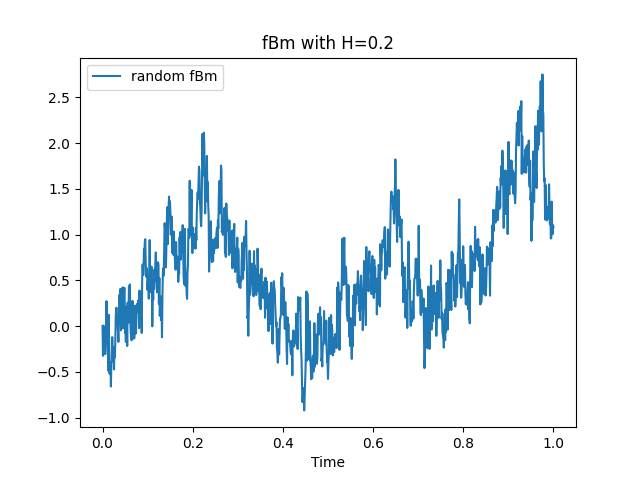
\includegraphics[width=65mm, height=65mm]{fBm_pictures/02.png} &   
  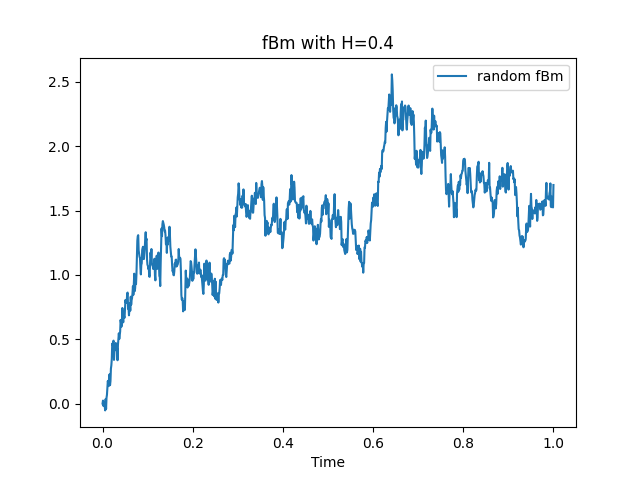
\includegraphics[width=65mm, height=65mm]{fBm_pictures/04.png} \\
(a) H=0.2 & (b) H=0.4 \\[6pt]

\end{tabular}
\end{figure}

% continued float ci fa spezzare le immagini in due pagine.
% poi setta l'altezza appropriata per mettere le immagini n pieno
\begin{figure}[ht] \ContinuedFloat
\begin{tabular}{cc}
 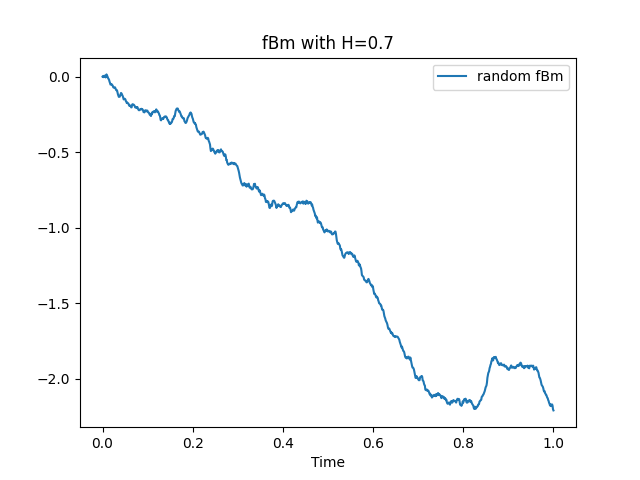
\includegraphics[width=65mm, height=62mm]{fBm_pictures/07.png} &   
 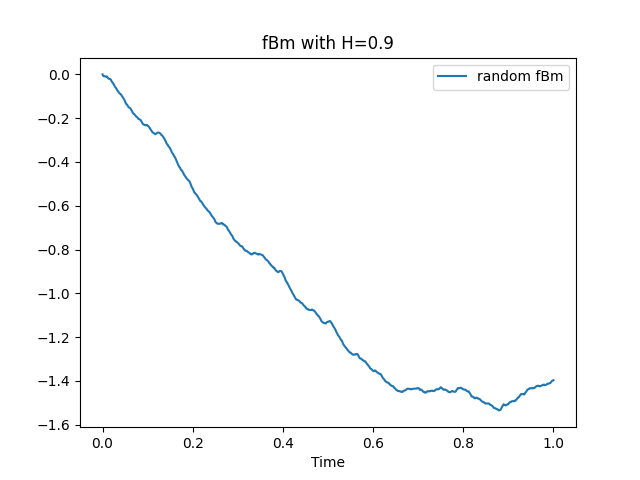
\includegraphics[width=65mm, height=62mm]{fBm_pictures/09.png} \\
(c) H=0.7 & (d) H=0.9 \\[6pt]
\multicolumn{2}{c}{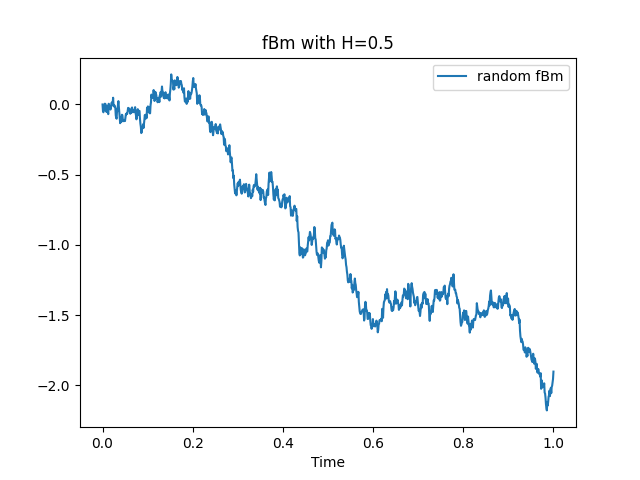
\includegraphics[width=65mm, height=62mm]{fBm_pictures/05.png} }\\
\multicolumn{2}{c}{(e) H=0.5 (standard Brownian motion)}
\end{tabular}
\caption{\label{fig:fBm}fractional Brownian motion's paths.}
\end{figure}
%referencing figure
%\eqref{fig:fBm}

\medskip
\medskip

As we can see from the plots, the sample paths of $W^H$ are at most $H-$Hölder continuous. As we get closer to $H=1$, the paths become smoother. 

We have a very rough behaviour when $H$ is small: when $H<\frac{1}{2}$, we say that the trajecories of the fractional Brownian motion have a \texit{``rough behaviour"}.\\
There is also the plot of a standard Brownian motion with $H=\frac{1}{2}$, Figure 
$1.1$ (e). \\

We can also observe the long-range memory effect: when $H$ is small, the range of values assumed by $W^H$, when the time is between $0$ and $1$, is wider than the range of values assumed by $W^H$ with higher $H$. This makes sense, as with higher values of $H$, the fBm $W^H$ has better memory of the past. Hence it is expected that it ``should not" move too far from previous values in a short time lapse. 

Finally we can visualize the reasons for which we denote the case $H<\frac{1}{2}$ as ``rough behaviour" of the fractional Brownian motion, while the case $H>\frac{1}{2}$ is known as the ``long memory behaviour".




\section{Riemann-Liouville integrals and derivatives of order $\alpha$}


Fractional derivatives (and integrals) refer to derivatives of order $\alpha$ where $\alpha$ is a real positive number not necessarily integer. There are various definitions of fractional derivatives and
integrals. We will discuss the Riemann-Liouville (henceforth R-L) integrals and derivatives, which were, as the name suggests, introduced by Riemann and Liouville. 

These generalize the concept of differentiation and integrals. \\ Linearity and semigroup properties are mantained. Moreover, the fractional R-L differential and integral operators are one the inverse of the other. 
\\
We will see some key properties. For further details see \cite{libro19}.\\

\noindent
We start by reminding:

\begin{definition}[Gamma Function]
\\\
\\
The Gamma function $\Gamma:\mathbb{C} \to \mathbb{R}$ is defined as 
\begin{equation}
\label{eq: gammafunction}
\Gamma(z) := \int_{0}^\infty x^{z-1}e^{-x}dx
\end{equation}
where $x$ is the real part of $z$.
\end{definition} 
\\
\noindent
When we want to integrate $n$ times, there is the known formula (Cauchy formula for repeated integration, see \cite{wikipediaCauchy}):

\begin{equation}
    \label{eq: nfold}
    \int_a^x \, d\sigma_1 \int_a^{\sigma_1 } \,d\sigma_2 ... \int_a^{\sigma_{n-1}} f(\sigma_n)\, d\sigma_n = \frac{1}{(n-1)!}\int_a^x (x-t)^{n-1}f(t)\,dt.
\end{equation}
And we remind that the Gamma function is strictly related to the factorial: $\Gamma(n) = (n-1)!$. Therefore, the RHS of \eqref{eq: nfold} might be generalized to the case $n\in \mathbb{R}_+$. Hence the definition from Riemann and Liouville:

\begin{definition}[Riemann-Liouville fractional integral of order $\alpha>0$]
\\\
\\
Given $\alpha>0$, $t>0$ and $f\in L^1(0,T)$, the Riemann-Liouville fractional integral of order $\alpha$ is defined as: 
\begin{equation}
    \label{eq: integralalfa}
    I_{\alpha} f(t) := \frac{1}{\Gamma(\alpha)}\int_{0}^t (t-s)^{\alpha-1} f(s)\,ds, \hspace{1cm} t\in (0,T)
\end{equation}


\end{definition}
\\\

In some books, the operator $I_\alpha$ is also denoted as $D^{-\alpha}$ (being the inverse of the fractional derivative $D^\alpha$ that we are going to define), or $I^{\alpha}$. We will stick to $I_\alpha$ as in the main paper \cite{Main} on which is based our work. 
Recall that $f\in L^1(0,T)$ iff $\int_0^T |f(x)|\, dx <\infty$.
\\
Notice that this definition generalizes the case with standard integrals, as for $\alpha$ integer we have exactly the formula \eqref{eq: nfold}.
\\\
\begin{remark}[Some useful properties of the R-L fractional integral operator]
\\\
\\
\textit{
$\bullet$ Notice that the R-L fractional integral operator $I_\alpha$ is a linear operator, as $I_\alpha (f + k g ) = I_\alpha (f) + k I_\alpha(g)$ for any $k\in R$ and $f,g\in L^1(0,T)$. The linearity follows immediately from the linearity of the standard integration.
\\
$\bullet$ It holds: 
\begin{equation}
    \label{eq: semigroupI}
    I_\alpha I_\beta = I_{\alpha + \beta}
\end{equation}
for any $\alpha,\beta >0$. 
}
\\
\\
For proof we refer to \cite{libro19}, Part $I$, section $2.3$. This makes of the set $\left\{ I_\alpha | \alpha>0 \right\}$, a semigroup with respect to the composition operation (induced by the composition of functions' operation) and
more importantly it makes of $\alpha \to I_\alpha$ a group homomorphism (where the space $\left\{ \alpha >0\right\}$ is given with the usual sum operation).
\end{remark}
\\\

It is then natural to define the R-L fractional derivative as the inverse operation of the fractional integral (from now on we might omit the ``Riemann-Liouville" connotation, as it is 
clear we only work with these fractional derivatives and integrals).\\\

We follow the approach from \cite{libro19}: we first define the fractional derivative for $\alpha \in (0,1)$, then we extend it to $\alpha \ge 1$.

\begin{definition}[Riemann-Liouville fractional derivative of order $\alpha\in (0,1)$]
\label{definition: riemannliouville deriv}
\\
Let $\alpha \in (0,1)$ and $t>0$. Given a function $f:(0,+\infty) \to \mathbb{R}$, we denote by 
\begin{equation}
    \label{eq: fractional.derivative}
    D^\alpha f(t) := \frac{1}{\Gamma(1-\alpha)} \frac{d}{dt} \int_0^t (t-s)^{\alpha-1}f(s)\,ds
\end{equation}
the Riemann-Liouville fractional derivative of $f$ of order $\alpha$, when it exists. 
\end{definition}
\\
\\
A sufficient condition for its existence is $f\in AC([0,T])$ (see Lemma 2.2 of \cite{libro19}).
\\

Now if we want to extend the definition to $\alpha \ge 1$, we have to consider some things: we would like that the fractional derivation is a generalization of the usual differentiations ($\alpha$ integer), and that the fractional derivatives operators satisfy the semigroup property, namely $D^\alpha D^\beta = D^{\alpha + \beta}$. \\
\\
Thus it is natural to define the fractional derivative for $\alpha \ge 1$ as: 
\begin{equation}
    \label{eq: fractional.deriv.2}
    D^\alpha f(t) := \left(\frac{d}{dx}\right)^{\lfloor \alpha \rfloor} D^{\left\{ \alpha \right\}} f(t)
\end{equation}
where $D^{\left\{ \alpha \right\}} f(t)=  \frac{1}{\Gamma(1-\left\{\alpha\right\})} \frac{d}{dt} \int_0^t (t-s)^{\left\{\alpha\right\}-1}f(s)\,ds$ by Definition \ref{definition: riemannliouville deriv}, as $0\le \left\{ \alpha \right\} <1$.
\\
\\
We can write \eqref{eq: fractional.derivative}  and \eqref{eq: fractional.deriv.2} in a more concise way. In general, the R-L fractional derivative of order $\alpha >0$ is

\begin{definition}[Riemann-Liouville fractional derivative of order $\alpha\in \mathbb{R}_+$]
We denote by
\begin{equation}
    \label{eq: fractional.deriv.general}
    D^\alpha f(t) = \frac{1}{\Gamma(n-\alpha)}\frac{d^n}{dt^n} \int_0^t (t-s)^{n-1-\alpha}f(s)\,ds, \hspace{0.5cm} n = \lfloor \alpha \rfloor+1
\end{equation}
the Riemann-Liouville fractional derivative of order $\alpha\in \mathbb{R}_+$ of $f$, when it exists.
\end{definition}

A sufficient condition for its existence is $f(x) \in AC^{\lfloor \alpha \rfloor}(0,T)$  (see \cite{libro19}, Chapter $I$, Theorem $2.2$).

This operator is an extension of the usual differential operator. Moreover, it satisfies the property $D^{\alpha + \beta} = D^\alpha D^\beta$ for all $\alpha, \beta>0$, as a direct consequence of how it has been defined. 
\\

Finally, the fractional differential operator $D^\alpha$ is indeed the inverse of the $I_\alpha$ operator. In particular it holds that
\begin{remark}[Reciprocal operators]
\begin{equation}
    \label{eq: inverseDF}
    D^\alpha I_\alpha(f) = f 
\end{equation}
for any $\alpha >0$, and for any $f$ for which it makes sense applying the operators $D^\alpha$ and $I_\alpha$ one after the other.
\end{remark}
\\\
This is a consequence of the Abel's equations (see \cite{libro19}, Chapter $I$, section $2.3$).
\\
However, it is not true that $I_\alpha D^\alpha(f)=f$. In the standard case, differentiating and then integrating a function, returns a function that differs by some constant to the initial function. 
In the same way, in the fractional case we do not have the identity $I_\alpha D^\alpha(f) = f$. \\ What we have instead is an expression like
\begin{equation}
    \label{eq: integrateafterdifferentiate}
    I_\alpha D^\alpha f = f + k_\alpha
\end{equation}
where $k_\alpha$ is linear combination of fractional monomial of the type $x^{\alpha - m}$, for $m=1,2,\cdots, \lfloor \alpha \rfloor +1$. For more details, see \cite{libro19} Chapter 2.6.
 

\subsection{Fractional derivatives and integrals of powers}

We will see now fractional derivatives and integrals of some elementary functions, in particular for $f(t) = t^r$ where $r\in \mathbb{R}$. 
\\\

\begin{lemma}[Fractional Derivative and Integral of Power functions]
\label{lemma: identities fract}
\\\
\\
The followings two hold true:
\begin{identity}[Fractional Derivative of Power functions]
\begin{equation}
    \label{eq: derivativePower}
    D^\alpha t^r = \frac{\Gamma(r+1)}{\Gamma(r+1-\alpha)} t^{r-\alpha} 
\end{equation}
if $r>\alpha - 1$ and $D^\alpha t^{\alpha-1} = 0$.
\end{identity}
\noindent
\begin{identity}[Fractional Integral of Power functions]
\begin{equation}
    \label{eq: integralPower}
    I_\alpha t^r = \frac{\Gamma(r+1)}{\Gamma(r+\alpha+1)} t^{\alpha+r} 
\end{equation}
if $r\ne -1$.
\end{identity}
\end{lemma}
Note that the fractional integral and derivative of a power function still remains a power function, modulo some constant. 
This justifies the use of fractional power series in trying to solve the Riccati equations as we will see later in this work.
\begin{proof} of Lemma \ref{lemma: identities fract}
\\\
\noindent
Let us prove \eqref{eq: integralPower} by direct computations:
by definition of fractional integral applied to $f(t)= t^r$ ($r \ne -1$), we have:
\begin{equation}
    \label{eq: UseleSSSforThen}
    I_\alpha f(t) = \frac{1}{\Gamma(\alpha)} \int_0^t (t-s)^{\alpha-1} s^r \, ds
\end{equation}
Now let us group the factor $t$ inside the integral:
$$ I_\alpha f(t) = \frac{1}{\Gamma(\alpha)} \int_0^t \left(1-\frac{s}{t} \right)^{\alpha-1} \left( \frac{s}{t} \right) ^r t^{\alpha+r-1}\, ds . $$
Now define $z:=\frac{s}{t}$ and get
$$ I_\alpha f(t) = \frac{1}{\Gamma(\alpha)} \int_0^1 (1-z)^{\alpha-1} z^r t^{\alpha+r} \, dz = \frac{1}{\Gamma(\alpha)}  t^{\alpha+r} \int_0^1 (1-z)^{\alpha-1} z^r \, dz.$$
We recognize the Beta function:
$$ I_\alpha f(t) = \frac{1}{\Gamma(\alpha)} B(r + 1, \alpha) t^{\alpha+r}$$
and by using the property $B(x,y) = \frac{\Gamma(x) \Gamma(y)}{\Gamma(x+y)}$, we get
$$ I_\alpha f(t) = \frac{1}{\Gamma(\alpha)} \frac{\Gamma(\alpha) \Gamma(r+1)}{\Gamma(\alpha+r+1)} t^{\alpha+r} = \frac{\Gamma(r+1)}{\Gamma(\alpha +r +1)} t^{\alpha+r}  $$
which is equation \eqref{eq: integralPower}.

The differential version \eqref{eq: derivativePower} is then a direct consequence of \eqref{eq: integralPower} together with the inversion formula $D^\alpha I_\alpha f = f$. 

\end{proof}

\subsection{Rewriting in integral form the Riccati differential equation}

Following the work of \cite{Main}, instead of working with the Riccati in its differential form, we will be working with the equivalent integral version. 
In particular, under appropriate integrability conditions on the functions $\psi^2$ and $\psi$, we have the equivalent integral Riccati equations.

For $\alpha \in (0,1]$, the Riccati differential equation $\mathcal{E} ^u_{\lambda , \mu , \nu}$ (defined in eq. \eqref{eq: fractionalRiccati}), becomes:
\begin{equation}
   \label{eq: integralRicc1}
   \psi(t) = \frac{u}{\Gamma(\alpha)} t^{\alpha-1} + I_\alpha (\lambda \psi^2 + \mu \psi + \nu ),
\end{equation}
while for $\alpha \in (1,2]$, the Riccati differential equation $\mathcal{E} ^ {u,v}_{\lambda, \mu , \nu }$ becomes the equivalent integral Riccati equation:
\begin{equation}
    \label{eq: integralRicc2}
     \psi(t) = \frac{u}{\Gamma(\alpha)} t^{\alpha-1} + \frac{v}{\Gamma(\alpha-1)} t^{\alpha - 2} + I_\alpha (\lambda \psi^2 + \mu \psi + \nu ).
\end{equation}

Notice that when we integrate we introduce the initial conditions inside the equations through the inversion formula \eqref{eq: integrateafterdifferentiate}, by considering that, $I_{1-\alpha} \left( \frac{u}{\Gamma(\alpha)} t^{\alpha-1} \right) = u$ and $I_{2-\alpha} \left( \frac{v}{\Gamma(\alpha)} t^{\alpha-2} \right) = v$ due to the integral formula for power series \eqref{eq: integralPower}.



\chapter{Riccati's solution as Power Series }
In this chapter we will express the solution to the Riccati fractional differential equation $\mathcal{E} ^ 0 _ {\lambda, \mu ,\nu}$ (eq. \eqref{eq: fractionalRiccati}), namely with $\alpha\in (0,1]$ and null initial condition $I_{1-\alpha} \psi(0)=0$, as a fractional power series. The homogeneous case (i.e., null initial condition) is simpler than the non-homogeneous case, which is solved through a double index series in \cite{Main}. 
Moreover, the homogeneous case has wider applications in Finance than the non-homogeneous case. \\
As anticipated at the beginning, the Riccati differential equation $\mathcal{E} ^ {u,v}_ {\lambda, \mu ,\nu}$ (defined in eq. \eqref{eq: fractionalRiccati}) has a unique solution (see \cite{Omar}). 

If we denote by $D_\psi$ the maximal domain of existence for the solution $\psi$ to $\mathcal{E} ^ 0 _ {\lambda, \mu ,\nu}$, and $R_\psi$ the radius of convergence of the fractional power series solution, then $\mathcal{D}(0,R_\psi) \subseteq D_\psi$ (where $\mathcal{D}(0,R_\psi)$ denotes the open disk centered in $0$ of radius $R_\psi$).
In particular the solution could exist outside the convergence radius of the fractional series. 
In this case we will use the Euler scheme (illustrated in the next chapter), which is a method that approximates the solution $\psi(t)$ to the Riccati differential equation with a sequence $\left\{ \bar{\psi}^n \right\}_{n\ge 1}$ of discrete functions.
\\
\\
We will focus solely on the case $t\ge 0$ from now on, though general results related to convergence also hold for $t\in \mathbb{C}$.
\\
\\
Assume that 
\begin{equation}
    \label{eq: fractionalPowerSeries}
    \psi(t) = \psi_{\lambda ,\mu , \nu}(t) := \sum_{k = 0}^\infty a_k t^{k\alpha}
\end{equation}
is a solution to $\mathcal{E} ^ 0 _ {\lambda, \mu ,\nu}$: 
\begin{equation}
    \label{eq: firstRiccatiNullCondition}
    D^\alpha \psi (t) = \lambda \psi^2 + \mu \psi + \nu, \hspace{0.4cm} I_{1-\alpha}\psi(0) = 0, \hspace{0.2cm} \alpha \in (0,1].
\end{equation}
We will impose \eqref{eq: firstRiccatiNullCondition} on \eqref{eq: fractionalPowerSeries} so that we can find explicitly the coefficients $a_k$. 
This does not guarantee that $\psi(t)$ is a solution to \eqref{eq: firstRiccatiNullCondition}.
It does satisfy the necessary conditions for being a solution to \eqref{eq: firstRiccatiNullCondition}, but we are not sure that the series is a well defined function, as it might diverge for some $t \in \mathbb{R}_+$ (we are interested only in the positive real axis). 
We also need to check that its convergence radius is positive, so that it is at least well defined in a non empty disk, where it absolutely converges (for $|t|<R_\psi$, while for $t=R_\psi$ we do not know the behaviour a priori).
\\
We first find explicitly the coefficients $a_k$, subsequently we will discuss about the existence of the solution and the convergence radius.
\\\
\\
We first recall the Cauchy-Hadamard's formula for computing the radius of convergence $R_\psi$.

\begin{lemma}[Cauchy-Hadamard's formula.]
\label{lemma: cauchyHadamard}
\textit{The radius of convergence $R_\psi$ for the fractional power series $\psi(t) = \sum_{k\ge0} a_k t^{k\alpha}$ is given by the formula:}
\begin{equation}
    \label{eq: HadamardSformula}
    R\psi = \liminf_{k\ge 0} |a_k|^{-\frac{1}{\alpha k }}.
\end{equation}
\end{lemma}

\noindent
As a final observation, notice that if $\nu = 0$, then $\psi(t) \equiv 0$ satisfies $\mathcal{E}^0_{\lambda, \mu, \nu}$. 
By uniqueness we deduce that this is the only solution to the Riccati $\mathcal{E}^0_{\lambda, \mu, 0}$. So, from now on we will suppose $\nu \ne 0$.

\section{Finding the coefficients}

    Let us assume that the convergence radius $R_\psi >0$ (we will discuss it later), in which case, for $t \ge 0$ such that $R_\psi> t$, the series converges absolutely. Moreover, if $R_\psi>0$, it also makes sense to talk about the series $\psi ^ 2$, or the Cauchy product of the series $\psi(t)= \sum_{k = 0}^\infty a_k t^{k\alpha}$ with itself. Indeed, for any $t \ge 0$ s.t. $R_\psi> t$, the Cauchy product is well defined, as both the factors (in this case the same series) are absolutely convergent within the convergence radius (see Theorem $3.50$, p. 74 in \cite{wikipediaMertens}).
\\\
\\
Hence
\begin{equation}
    \label{eq: cauchyProductSquare}
    \psi^2(t) = \sum_{k\ge 0} a_k^{*2}t^{k\alpha},
\end{equation}
\\
where the coefficients $a_k^{*2}$ of the Cauchy product are given by the convolution of the coefficients $a_k$:
\begin{equation}
    \label{eq: coefficientsConvolution}
    a_k^{*2} = \sum_{l=0}^k a_l a_{k-l},  \hspace{0.3cm} k \ge 0.
\end{equation}
\noindent
Now, recalling the fractional derivative of a power function in equation \eqref{eq: derivativePower}, it follows that
\begin{equation}
    \label{eq: 17.9inThePaper}
    D^\alpha \psi(t) = \sum_{k\ge 0} a_k \frac{\Gamma(\alpha k +1)}{\Gamma(\alpha k + 1 - \alpha)} t^{\alpha (k-1)} 
\end{equation}
where $\alpha \in (0,1]$. Note that this is in analogy with the formal standard derivative of a series (for $|t| < R_\psi$, the formal derivative of a series is convergent, as it has the same radius of convergence $R_\psi$),
where in our case the fractional derivative of the series becomes a series of fractional derivatives.
\\
\\
Now, given the Riccati equation structure $\mathcal{E}^0_{\lambda, \mu, \nu}$ and \eqref{eq: cauchyProductSquare}, it follows that
\begin{equation}
    \label{eq: 18inThePaper}
    D^\alpha \psi(t) = \lambda \psi^2(t) + \mu \psi(t) + \nu = \sum_{k\ge 0} (\lambda a_k^{*2} + \mu a_k)t^{\alpha k} + \nu,
\end{equation}
\\
so that we can compare \eqref{eq: 18inThePaper} and \eqref{eq: 17.9inThePaper} and equate the coefficients that have the same power $t^{\alpha k}$. This is justified by the theory of complex series within their convergence radius, namely, if two series are equal within a portion of their convergence domain, then their coefficients are equal in that portion of domain. 
Comparing the two series gives us a recurrent relation on the coefficients $a_k$:
\begin{equation} 
    \label{eq: recurrent1}
    (A_{\lambda, \mu, \nu} ) \equiv
    \begin{cases}
    a_{k+1} = (\lambda a_k^{*2} + \mu a_k) \frac{\Gamma(\alpha k +1)}{\Gamma(\alpha k + \alpha  +1)}, \hspace{0.2cm} k\ge 1,
    \\
    a_1 = \frac{\nu}{\Gamma(\alpha+1)}, 
    \\
    a_0 = 0,
    \end{cases}
\end{equation}
where we recall that $a_k^{*2}$ solely depends on the coeffients $a_l$ for $l\le k$.
\\
The relation $(A_{\lambda, \mu, \nu} )$ determines uniquely the coefficients $a_k$ of the fractional power series. 
Notice also that since $a_0=0$, then $\psi(0)=0$, which is our initial condition.


\section{Radius of Convergence}

So far we assumed that the radius of convergence $R_\psi$ is greater than zero in order to find the relations on the coefficients $a_k$ given in $(A_{\lambda, \mu, \nu} )$. The fact that $R_\psi>0$ is justified by the following theorem, whose proof will be omitted (for reference see \cite{Main}):

\begin{theorem}\label{th: importantTheorem}
Let $\alpha \in [0,2]$, $\lambda, \mu, \nu \in \mathbb{C}$ and $\lambda \ne 0$. Let $\psi_{\lambda, \mu , \nu} = \sum_{k\ge 0} a_k t^{k\alpha}$, where the coefficients $a_k$ satisfy \eqref{eq: recurrent1}. Then
\\
i) [lower bound radius] we have
\begin{equation}
    \label{eq: 22inThePaper}
     0< \tau_* := \frac{2^{\frac{1}{\alpha} - (\frac{1}{\alpha} - 2)^+}\alpha}{\left( |\mu|  +\sqrt{\mu^2 + c_\alpha \frac{|\lambda||\nu|}{\Gamma(\alpha)}}\right) ^\frac{1}{\alpha} } < R_{\psi_{\lambda, \mu, \nu}}
\end{equation}
where $c_\alpha = 2^{2-(1-2\alpha)^+ - 2(\alpha -1)^+}\alpha ^{\alpha-1} B(\alpha \wedge 1, \alpha \wedge 1) >0$. Notice that $\tau_{*}$ depends only on the coefficients of the Riccati equation and on the order of differentiation $\alpha$.
\\
\\
ii) [upper bound radius] 
if $\mu \ge 0$, $\lambda,\nu >0$ (respectively $\mu \le 0$, $\lambda,\nu <0$), then


    
$$ R_{\psi_{\lambda, \mu, \nu}} \le R_{\psi_{|\lambda|, 0, |\nu|}}  \le C_\alpha \left( \frac{\Gamma(\alpha+1)}{\lambda \nu}\right) ^ \frac{1}{2\alpha}$$
where
$$C_\alpha = \begin{cases}
(3.5^{\alpha-1})*\frac{1}{2\alpha}\sqrt{\alpha} & if \hspace{0.1cm} \alpha \in (0,1]
\\
\tfrac{\sqrt{2\alpha}}{\Tilde{B}(\alpha)} & if \hspace{0.1cm}  \alpha \in (1,2]
\end{cases} $$
where $\Tilde{B} (\alpha) = B(\alpha,\alpha) - 2^{1-2\alpha} >0. $ Moreover, $\psi_{\lambda, \mu, \nu}$ is increasing (respectively decreasing) for t such that $R_{\psi_{\lambda,\mu,\nu}}> t\ge 0$. And we also have 
$$\lim_{t\to +R_{\psi_{\lambda,\mu,\nu}}} \psi_{\lambda,\mu,\nu}(t) = sgn(\lambda) \cdot \infty.$$
\end{theorem}
\\\
\\
This theorem grants us that the radius of convergence is positive if $\lambda \ne 0$. 
We wonder what happens if $\lambda = 0$.

\subsection{Particular Case $\lambda = 0$}
\\
If $\lambda = 0$, then we will show that the radius of convergence $R_\psi = +\infty$ (i.e., the series converges absolutely everywhere).

Let $\lambda = 0$, then by $(A_{\lambda, \mu, \nu})$ we easily get by induction
\begin{equation}
    a_{k+1} = \nu  \frac{\mu^k}{\Gamma(\alpha (k+1)+1)}, 
\end{equation}
\noindent
for any $k\ge 1$. In particular, if $\mu =0$ then $a_{k+1}\equiv 0$ for any $k\ge 1$. Thus the series converges absolutely everywhere ($R_\psi =+\infty$). Assume now $\mu \ne 0$.
\\
\\
Consider the limit
\begin{equation}
\label{eq: lambda0Partic}
\begin{gathered}
\lim_{k\to +\infty} |a_{k}|^{-\frac{1}{\alpha k}} =  \\
\lim_{k\to +\infty} \left( \frac{|\nu| |\mu|^{k-1}}{\Gamma(k\alpha +1)} \right)^{-\frac{1}{\alpha k}} = \\
\lim_{k\to +\infty}
\frac{1}{|\mu|^{\frac{k-1}{\alpha k}}} \cdot \frac{1}{|\nu|^{\frac{1}{\alpha k}}} \cdot \left( \Gamma(\alpha k +1) \right)^{\frac{1}{\alpha k}}.
\end{gathered}
\end{equation}
\noindent
We want to prove that this limit \eqref{eq: lambda0Partic} is $+\infty$, which, by Hadamard's formula (Lemma \ref{lemma: cauchyHadamard}) means $R_\psi = +\infty$.
\\
\\
The first product $\frac{1}{|\mu|^{\frac{k-1}{\alpha k}}} \cdot \frac{1}{|\nu|^{\frac{1}{\alpha k}}}$ converges to $\frac{1}{|\mu| ^ \frac{1}{\alpha}} > 0$ as $k\to +\infty$ (remind that $\alpha \in (0,2)$ and $\mu, \nu \ne 0$):
$$\lim_{k\to +\infty} \frac{1}{|\mu|^{\frac{k-1}{\alpha k}}} \cdot \frac{1}{|\nu|^{\frac{1}{\alpha k}} } = \frac{1}{|\mu| ^ \frac{1}{\alpha}} > 0.$$ 
Thus, the limit \eqref{eq: lambda0Partic} is $+\infty$, if and only if,  $\left( \Gamma(\alpha k+1) \right)^{\frac{1}{\alpha k}} \to +\infty$ as $k\to +\infty$. 
In order to prove this, we will show the following:

\begin{corollary}
\label{corollary: usefulFormulaForGamma}
\\\
\\\
Let $\Gamma$ be the Gamma function. Then 
\begin{equation}
    \label{eq: strangeCorollaryGammaFun}
    \lim_{x \to +\infty} \Gamma(x) ^{\frac{1}{x-1}} = +\infty.
\end{equation}
\end{corollary}
\\

It is clear that if this holds, then the limit \eqref{eq: lambda0Partic} converges to $+\infty$ (set $x:=\alpha k + 1$, then $\left( \Gamma(\alpha k+1)  \right)^{\frac{1}{\alpha k}} = \Gamma(x) ^{\frac{1}{x-1}} $).
\\
\\
In order to prove Corollary \ref{corollary: usefulFormulaForGamma}, we will use Nemes' formula (Corollary $4.1$ from \cite{nemesGamma}):
\begin{corollary}[Nemes' formula]
\label{corollary: nemesFormula}
\\\
\\\
Let $\Gamma$ be the Gamma function. Then, for $x\to +\infty$, it holds the following asymptoticity:
\begin{equation}
    \Gamma(x) \sim \left( \frac{x}{e} \right)^x \sqrt{\frac{2\pi}{x}} \left( 1+ \frac{1}{12x^2-\frac{1}{10}}\right)^x.
\end{equation}
\end{corollary}


\noindent
Now let us prove Corollary \ref{corollary: usefulFormulaForGamma}.
\begin{proof} of Corollary \ref{corollary: usefulFormulaForGamma}.
\\
\noindent 
Using Nemes' formula (Corollary \ref{corollary: nemesFormula}) we get, for $x\to +\infty$:
\begin{equation}
\label{eq: gammaAsymptoticityNemes}
    \Gamma(x) ^ {\frac{1}{x-1}} \sim \frac{x^{\frac{x-\frac{1}{2}}{x-1} }}{e^{\frac{x}{x-1}}} \cdot \sqrt{2 \pi}^{\frac{1}{x-1}} \cdot \left( 1+ \frac{1}{12x^2 - \frac{1}{10}} \right)^{\frac{x}{x-1}}.
\end{equation}
\noindent
It is clear that the product $ \frac{x^{\frac{x-\frac{1}{2}}{x-1} }}{e^{\frac{x}{x-1}}} \cdot \sqrt{2 \pi}^{\frac{1}{x-1}}$ converges to $+\infty$ as $x\to +\infty$:
\begin{equation}
\label{eq: firstProdGammaAsymp}
    \lim_{x \to +\infty} \frac{x^{\frac{x-\frac{1}{2}}{x-1} }}{e^{\frac{x}{x-1}}} \cdot \sqrt{2 \pi}^{\frac{1}{x-1}} = +\infty,
\end{equation}
\noindent
and $\left( 1+ \frac{1}{12x^2 - \frac{1}{10}} \right)^{\frac{x}{x-1}}$ converges to $1$ as $x\to +\infty$:
\begin{equation}
\label{eq: secondProdGammaAsymp}
    \lim_{x\to +\infty} \left( 1+ \frac{1}{12x^2 - \frac{1}{10}} \right)^{\frac{x}{x-1}} = 1.
\end{equation}
\noindent
Finally, using \eqref{eq: gammaAsymptoticityNemes}, \eqref{eq: firstProdGammaAsymp} and \eqref{eq: secondProdGammaAsymp}, we get:
$$
    \lim_{x\to +\infty} \Gamma(x) ^{\frac{1}{x-1}} = \lim_{x \to +\infty} \frac{x^{\frac{x-\frac{1}{2}}{x-1} }}{e^{\frac{x}{x-1}}} \cdot \sqrt{2 \pi}^{\frac{1}{x-1}} \cdot \left( 1+ \frac{1}{12x^2 - \frac{1}{10}} \right)^{\frac{x}{x-1}} = +\infty,
$$
\\
\noindent
which is \eqref{eq: strangeCorollaryGammaFun}. 
\end{proof}

This concludes the fact that $\lambda = 0$ implies $R_\psi = +\infty$, namely, the series converges absolutely everywhere.

\subsection{About Accuracy and Truncation of the series}
\\
There is a final note about the accuracy in truncating the fractional power series, as making numerical tests will not allow us to have infinite sums. 
In this regard, there are some estimates that measure the accuracy of the fractional power series truncated up to the $n_0$-th coefficient (we will consider $\sum_{k=0}^{n_0}$ $a_kt^{k\alpha}$ in place of $\sum_{k=0}^{+\infty} a_kt^{k\alpha})$. 
The accuracy, or relative distance from the real value, is affected by $n_0$. Later we will see the formula \eqref{eq: accuracyTruncation}, which gives the least $n_0$-th coefficient up to which we have to truncate the series in order to attain a desired accuracy $\epsilon_0 \ge 0 $. For further details see \cite{Main}. 
\\

Recapitulating, by imposing $\mathcal{E}^0_{\lambda, \mu, \nu}$ on $\psi(t)= \sum_{k\ge 1} a_k t^{k\alpha}$, we determined the coefficients $a_k$ (a recurrent relation $(A_{\lambda, \mu,\nu})$ on $a_k$). 
Moreover, since the convergence radius is positive by Theorem \ref{th: importantTheorem}, the series $\psi(t)= \sum_{k\ge 1} a_k t^{k\alpha}$ is well defined within its convergence radius. 
Therefore, for $|t|<R_\psi$, the series whose coefficients are determined by $(A_{\lambda, \mu,\nu})$, satisfies to $\mathcal{E}^0_{\lambda, \mu, \nu}$ (by construction), being then a solution.
Nevertheless, knowing that the solution exists and it is unique (see \cite{Omar}), this has to be exactly the solution.

There is a limitation in this: the fractional power series centered at zero is only defined within $R_\psi$, while the solution might exist over $R_\psi$. For this we will apply an hybrid approach in Chapter \ref{chapter: eulerDiscretizationScheme}.


\chapter{Euler Discretization Scheme}
\label{chapter: eulerDiscretizationScheme}

In the previous chapter we expressed the solution to $\mathcal{E}^0_{\lambda, \mu, \nu}$ (eq. \eqref{eq: fractionalRiccati}) as a fractional power series. 
However, the solution could be defined in a larger domain than the power series' domain of absolute convergence (i.e., a disk centered in $0$). 
For this reason we apply an Euler scheme that approximates the solution $\psi$. 
This scheme aims to define the solution in a broader domain through a sequence of piecewise step functions $\left\{ \bar{\psi}^n \right\}_{n \in \mathbb{N}}$ that converges to the solution $\psi$. 
The whole approach will be hybrid in the sense that within a threshold (to be specified as below in Section \ref{section: hybrid expansion threshold}) we still use the fractional power series, while outside of that threshold we will use the Euler scheme.
\\

We remind that we focus our analysis for $T>0$ such that $T\in D_\psi$ (i.e., $T$ is in $D_\psi$, the maximal domain of existence of the solution).
For such a $T>0$ fixed, we will approximate $\psi(T)$ with some functions $\bar{\psi}^n(T)$ that converge to $\psi(T)$ as $n\to + \infty$. 
\\
\\
We recall that
$$ \psi(t)= \sum_{r\ge 1} a_r t^{\alpha r} $$
within the disk $\mathcal{D}(0,\widehat{R_\psi})$. 
From this we get, reminding the identity for fractional integrals of power functions \eqref{eq: integralPower} and letting $f_r(t) := t^{r\alpha}$:
\begin{equation}\label{eq: 27inthepaper}
\begin{aligned} 
    I_{1-\alpha}(\psi)(t) &= \sum_{r\ge 1} a_r I_{1-\alpha}(f_r)(t)
    \\
    &= \sum_{r\ge 1} a_r \frac{\Gamma(\alpha r + 1)}{\Gamma(\alpha r - \alpha + 1)}\cdot \frac{t^{\alpha r + 1 - \alpha}}{(\alpha r + 1 - \alpha)} 
    \\
    &= t^{1-\alpha} \left( \nu t^\alpha  +\sum_{r=2}^\infty a_r \left(1-\frac{1}{r}\right)^{-1} \frac{\Gamma(\alpha r) t^{r\alpha}}{ \Gamma(\alpha r - \alpha) \cdot (\alpha r + 1 - \alpha)}  \right)
\end{aligned}
\end{equation}
\noindent
where in the last equality we substituted the values of $a_0$ and $a_1$ from $(A_{\lambda,\mu,\nu})$ in equation \eqref{eq: recurrent1}.
\\

In practical cases, we will be using Hadamard's formula to get an estimate of the radius of convergence $R_\psi$. Let us see how we estimate it.

\section{Estimates of the radius $R_\psi$ and accuracy}

We do not have only one way of estimating the radius of convergence $R_\psi$: we will discuss two estimates. Let us see into more details.

\subsection{Two estimates for the radius of convergence $R_\psi$ }
By Hadamard's formula, we know that the radius of convergence $R_\psi$ is given by
$$R_\psi := \liminf_{r\ge 0} |a_r|^{-\frac{1}{\alpha r}} = \lim_{r\to + \infty} \left( \inf_{m\ge r} |a_m|^{-\frac{1}{\alpha m}}\right).  $$
Since we cannot compute all the coefficients $a_m$ ($m \in \mathbb{N}$), we will have to estimate $R_\psi$. In particular, if we compute the first $r_{max}$ coefficients (where $r_{max} \in \mathbb{N}$ is arbitrary, even though later we pick it as in \eqref{eq: accuracyTruncation} with $r_{max} = r_0$, in order to attain a desired accuracy), we will have an estimate:\\
\\
\textbf{Estimate Radius 1.}
\begin{equation}
    \label{eq: estimateRadius4}
    R_\psi ^ {r_{max}} := |a_{r_{max}}|^ {-\frac{1}{\alpha_{r_{max}}}}
\end{equation}
Note that this might overestimate $R_\psi$, as well as underestimate it, as the sequence of coefficients $\left\{ a_m\right\}_{m\in \mathbb{N}}$ might not be monotone. \\ 
Now, if we consider the fractional series $I_{1-\alpha}(\psi)(t)$ (see \eqref{eq: 27inthepaper}), then this has the same radius of converence as of the fractional series $\psi(t) = \sum_{k\ge 0} a_kt^{k\alpha}$, by the general theory of complex power series (which also holds in the fractional case, as the fractional integral $I_{1-\alpha}$ is defined through standard integrations).
\\
If we denote by $a_r'$ the coefficients of the series $I_{1-\alpha}(\psi)(t)$ (see \eqref{eq: 27inthepaper}), then
\begin{equation}
\label{eq: aprimo_R_radius_convergence}
    a'_r = a_r\frac{\Gamma(\alpha r + 1)}{\Gamma(\alpha r - \alpha + 1)} \frac{1}{\alpha r + 1 - \alpha}.
\end{equation}
\\
Therefore we can have (see below eq. \eqref{eq: estimateRadiusAnother}) an alternative estimate $\widehat{R}_\psi$ for the radius $R_\psi$.
\\
\\
\textbf{Estimate Radius 2.} A second possible estimate is:
\begin{equation}
    \label{eq: estimateRadiusAnother}
    \widehat{R}_\psi := |a'_{r_{max}}|^ {-\frac{1}{\alpha r_{max}}}.
\end{equation}
% Notice that generally $a'_r \ge a_r$. This comes from the Gamma function property $\frac{\Gamma(\alpha + 1)}{\Gamma(\alpha)} = \alpha$, so that 
% \begin{equation}
% \begin{aligned}
% \frac{\Gamma(\alpha r + 1)}{\Gamma(\alpha r - \alpha + 1)} \frac{1}{\alpha r + 1 - \alpha} &= \alpha r \cdot (\alpha r - 1) \cdots (\alpha r - \alpha + 1 ) \frac{1}{\alpha r + 1 - \alpha} 
% \\
% &= \prod_{i=2}^{\alpha} (\alpha r - \alpha + i).
% \end{aligned}
% \end{equation}
% Which is usually greater than one for the values of $\alpha$ and $r$ ($r$ at least 100, and $\alpha\ge 0.6$) that we generally use in the Heston model in finance to reproduce the rough behaviour  ($H<\frac{1}{2}$ or $\frac{1}{2}<\alpha <1$. For more details see paper \cite{Main}).
% In particular, as a result of $a'_r \ge a_r$, it follows that
% $$ R^{r_{max}}_\psi = |a_{r_{max}}|^ \frac{-1}{\alpha r_{max}} \ge |a'_{r_{max}}|^ \frac{-1}{\alpha r_{max}} = \widehat{R}_\psi $$
% as $\alpha , r > 0$. \\
% This tells us that the estimate $\widehat{R}_\psi$ is more prone to underestimation than $R^{r_{max}}_\psi$. We prefer an underestimate of $R_\psi$ instead of an overestimate. 
\noindent
We prefer using this estimate $\widehat{R}_\psi$, as they do in paper \cite{Main}.

\subsection{Accuracy In truncating}
\label{subsection: accuracy in truncating}

So far, truncating and having an approximate radius of convergence is not enough: 
we also need a measure of accuracy for the truncated series, where by accuracy we mean the maximum relative distance to the real value inside the disk $\mathcal{D}(0,\widehat{R}_\psi)$. Namely, if we denote by $\tilde{\psi}(t) := \sum_{k = k_0}^n a_k t^{k\alpha}$ the truncated series and $\psi$ the solution to the Riccati equation $\mathcal{E}^0_{\lambda, \mu, \nu}$ (eq. \eqref{eq: fractionalRiccati}), then $d(\tilde{\psi}, \psi)(t) := 
\left| \frac{\tilde{\psi}(t)- \psi(t)}{\tilde{\psi}(t)} \right| $ is our precision in $t$, where $|t| < \widehat{R}_\psi$. The accuracy is the sup of the precisions in $t$ for $t\in \mathcal{D}(0,\widehat{R}_\psi)$: $\sup_{|t| < \widehat{R}_\psi}d(\tilde{\psi}, \psi)(t) $. Let $\epsilon_0$ be our accuracy (typically $\epsilon_0 = 0.01$).
If we want the value of the series in $t$, for $t$ close to the estimate $\widehat{R}_\psi$, we will need to compute more terms of the series in order to attain the desired precision, which is not uniform in $t$. For this reason we move a bit away from the threshold $\widehat{R}_\psi$, by taking $\theta \in (0,1)$ and considering the truncated series for $t\in [0, \theta \widehat{R}_\psi].$ Moreover the accuracy will be intended to the restricted disk $\mathcal{D}(0,\theta \widehat{R}_\psi )$. In the numerical tests in section \ref{section: generalprocedure} we use $\theta = 0.9$.
\\
\\
The desired accuracy is attained by truncating up to the first  $r_0$ coefficients, where $r_0$ is given by
\begin{equation}
    \label{eq: accuracyTruncation}
    r_0 = r_0(\epsilon_0, \theta) = \left\lceil \frac{log(\epsilon_0 (1-\theta))}{ \alpha \log (\theta)}  -1  \right\rceil
\end{equation}
\\
This formula is given in \cite{Main}, which is determined empirically.
\\
\\
Now we can proceed to our hybrid expansion with the Euler discretization scheme.

\section{Hybrid Expansion}
\label{section: hybrid expansion threshold}

As discussed in the previous subsection \ref{subsection: accuracy in truncating}, we keep us far from the estimate $\widehat{R}_\psi$ by setting the threshold to $\theta \widehat{R}_\psi$ in order to have enough accuracy in the series expansion. 
\\\
\\
If we want to compute $\psi(T)$, we have two cases based on the value of $T$ (which we remind being positive and belonging to $D_\psi$, the maximal domain of existence of the solution $\psi$.). 

\subsection{Case 1: $T< \theta \widehat{R}_\psi$.}
If $T< \theta \widehat{R}_\psi$,
we simply evaluate the truncated fractional power series (whose coefficients satisfy $(A_{\lambda, \mu, \nu} )$) in $T$ and set the result as the value assumed by $\psi(T)$.

\subsection{Case 2: $T >  \theta \widehat{R}_\psi$.}
\label{subsection: firstpsin}
If $T >  \theta \widehat{R}_\psi$,
we use the Euler discretization scheme, which we are going to introduce below.
\\ 
Let $n\ge1 $ be a fixed integer. We denote by $\bar{\psi}^n$ the $n$-th Euler discretization of $\psi$. This is an estimate of $\psi$ and is a piecewise step function assuming at most $n\in \mathbb{N}$ different values (namely, a finite linear combination of indicator functions of intervals). As $n$ increases, the estimate $\bar{\psi}^n$ becomes more and more accurate.\\

We divide the disk $\mathcal{D}(0,T)$ into circular areas with increasing radius of fixed step $h=\frac{T}{n}$, where $n\ge 1$ integer. 
We set  
\begin{equation}\label{eq: tk and k0}
     t_k = t_k^n := \frac{kT}{n}, \hspace{0.2cm} k=0,...,n, \hspace{0.4cm} and \hspace{0.2cm} k_0 := \left\lfloor \frac{n \theta \widehat{R}_\psi }{T}\right\rfloor.
\end{equation}
\\
Note that $k_0$ is such that $t_{k_0} \le \theta \widehat{R}_\psi <t_{k_0 +1}$, i.e. it is the largest integer s.t. $t_{k_0}$ is smaller than the threshold $\theta \widehat{R}_\psi$.  \\
The function $\bar{\psi}^n$ is a discrete function and first we define it in the set $\left\{t_k| k=0,...,n \right\}$, then we extend it to the whole interval $(t_0,t_n) = (0,T)$ as a piecewise step function (if $t\in [t_l,t_{l+1})$ we set $\bar{\psi}^n(t) = \bar{\psi}^n(t_l)$). \\

So how do we define the values of $\bar{\psi}^n(t_k)$ for $k=0,\cdots,n$?
\\
We use the power series expansion up to $  \theta \widehat{R}_\psi$. Subsequently, we consider the integral form of the Riccati  equation $(\mathcal{E} ^0_{\lambda, \mu, \nu})$, namely
$$ \psi = I_\alpha \left( \lambda \psi^2 + \mu \psi + \nu \right).$$
In particular, for the values $k$ such that $0 \le k\le k_0$, we set $\bar{\psi}^n(t_k)$ equal to the value computed with the fractional power expansion truncated at $r_0$ and evaluated at $t_k$.
\\
In order to compute the other values $\bar{\psi}^n (t_k)$, for $k \in \left\{ k_0+1, k_0+2, \cdots, n \right\}$, we use the following Euler Scheme:

\subsection{Euler Scheme}
\label{subsection: secondpsin}
\noindent
Given the integral form of the Riccati $\mathcal{E}^0_{\lambda, \mu, \nu}$:
\begin{equation}
    \label{eq: temporaryVariable3..2}
    \psi(t) = \frac{\nu t^\alpha}{ \Gamma(\alpha+1)} + \frac{1}{\Gamma(\alpha)} \int_0^t \psi(s) (\mu + \lambda \psi(s)) (t-s) ^ {\alpha - 1} \,ds,
\end{equation}
being $n$ fixed, we can compute the values $\bar{\psi}^n (t_k)$ for $k=k_0+1, \cdots , n$ by recurrence on $k\ge k_0+1$ through the formula:
\begin{equation}
\label{eq: 28inthepaper}
\begin{aligned}
    \bar{\psi}^n(t_k) &= \frac{\nu t_k^\alpha}{\Gamma(\alpha+1)} + \frac{1}{\Gamma(\alpha)} \sum_{l=1}^{k-1} \bar{\psi}^n(t_l) \left( \lambda \bar{\psi}^n(t_l) + \mu \right) \int_{t_l}^{t_{l+1}} (t_k - s)^{\alpha - 1} \, ds
    \\
    &= \frac{1}{\Gamma(\alpha + 1)} \left( \frac{t}{n}\right)^\alpha \left( \nu k^\alpha + \sum_{l=1}^{k-1} c_{k-l-1}^{(\alpha)}  \bar{\psi}^n(t_l) \left( \lambda \bar{\psi}^n(t_l) + \mu \right) \right)
    
\end{aligned}
\end{equation}
with
\begin{equation*}
    c_0^{(\alpha)} = 1 \hspace{0.3cm} and \hspace{0.4cm} c_l^{(\alpha)} = (l+1)^\alpha -l^\alpha, \hspace{0.2cm} for \hspace{0.2cm} l=1,\cdots, k-2.
\end{equation*}
This formula \eqref{eq: 28inthepaper} follows from the integral Riccati formula \eqref{eq: temporaryVariable3..2}. We substituted $t$ with $t_k$ and $\psi$ with $\bar{\psi}^n$. Then we know how $\bar{\psi}^n$ is defined up to $t_{k-1}$ and we can compute recursively the value in $t_k$, as $\bar{\psi}^n$ is a piecewise step function. \\\
Moreover, notice that the last equality in \eqref{eq: 28inthepaper} holds since
$$ \int_{t_l} ^ {t_{l+1}} (t_k - s ) ^ {\alpha -1} = \frac{(t_k-t_l)^\alpha - (t_k-t_{l+1})^\alpha}{ \alpha} = \left( \frac{t}{n}\right)^\alpha \frac{1}{\alpha} \left(  (k-l)^\alpha - (k-l-1)^\alpha \right)$$
where we used the definition of $t_k$ and the property of the Gamma function $\frac{\Gamma(\alpha)}{\Gamma(\alpha+1)} = \frac{1}{\alpha}$ for any $\alpha >0$.

\subsection{How good does $\bar{\psi}^n$ approximate $\psi$?}
\label{subsection: rrfirst_estimate}
\noindent
There is not a theoretical estimate yet, but sperimental tests strongly suggest that 
\begin{equation}
    \label{eq: 30inthepaper}
    \bar{\psi}^n(T) - \psi(T) = \frac{c_1}{n}+ o(n^{-1})
\end{equation}
for a constant $c_1$.
If this estimate holds true, we can also estimate the value of $c_1$.
\begin{remark} \label{remark: c1_series}
\textit{Assuming the validity of \eqref{eq: 30inthepaper}, we get that the sequence $\left\{ \bar{c_1}^n \right\}_{n\in N}$ defined as
\begin{equation}
    \label{eq: 32inthepaper}
    \bar{c}_1^n := 2n \left( \bar{\psi}^n(T) - \bar{\psi}^{2n}(T) \right)
\end{equation}
convergese to $c_1$ as $n\to +\infty$.}
\end{remark}
\\
Indeed
\begin{equation*}
\begin{aligned}
    \bar{c}_1^n &= 2n \left( \bar{\psi}^n(T) - \bar{\psi}^{2n}(T) \right) \\
    &= 2n \left( \left( \bar{\psi}^n(T) - \psi(T) \right)  - \left( \bar{\psi}^{2n}(T) - \psi(T) \right)\right) \\
    &= 2n\left( \frac{c_1}{n} -\frac{c_1}{2n}  + o(n^{-1})\right)\\
    &= c_1 + 2n\cdot o(n^{-1}) \to c_1
\end{aligned}
\end{equation*}
as $n\to \infty$ since $n \cdot o(n^{-1}) \to 0$ as $n\to \infty$.
\\\

Summarizing, we approximated $\psi(T)$ with $\bar{\psi}^n(T)$ through an hybrid method consisting of the fractional series expansion and the Euler scheme. 
Having the estimate $\bar{\psi}^n(T)$ of $\psi(T)$ is yet a considerable result, especially for large values of $n$. 
Nevertheless we can have a faster convergence through an extrapolation if the measure \eqref{eq: 30inthepaper} holds true. This happens with the extrapolated hybrid method that we will see in the next section:

\section{Extrapolated Hybrid Method}
\label{section: extrapolatedhyb}
If we assume the error estimate \eqref{eq: 30inthepaper}, then, from the hybrid Euler expansion we can get an approximator for $\psi(T)$, namely the 
(single step) Richardson-Romberg Approximator:
\begin{equation}
    \label{eq: RR.1}
    \bar{\psi}^n_{_{RR,2}}(T) := 2 \bar{\psi}^n(T) - \bar{\psi}^{\frac{n}{2}}(T)
\end{equation}
defined for $n$ even.
\\\
\\
The Richardson-Romberg approximator $\bar{\psi}^n_{_{RR,2}}(T)$, extracted from the Euler approximator $\bar{\psi}^n(T)$, converges faster than the latter. Indeed it holds that

\begin{equation*}
    \begin{aligned}
    \bar{\psi}^n_{_{RR,2}}(T) - \psi(T) &= 2\left( \bar{\psi}^n(T) - \psi(T) \right) - \left( \bar{\psi}^{n/2}(T) - \psi(T) \right) \\
    &= 2\left( \frac{c_1}{n} + o(n^{-1}) \right) - \left( \frac{c_1}{n/2} +o(n^{-1}) \right) 
    \\
    &= o(n^{-1}),
    \end{aligned}
\end{equation*}
which goes to zero faster than \eqref{eq: 30inthepaper}, as $n\to +\infty$, meaning that the Richardson-Romber approximator $\bar{\psi}^n_{_{RR,2}}(T)$ converges to the solution $\psi$ more quickly than the Euler approximator $\bar{\psi}^n$.

\subsection{Multistep extrapolated hybrid method}
\label{subsection: multiStepRR}

Let us assume that in place of \eqref{eq: 30inthepaper} there is a more accurate estimate of the error, namely
\begin{equation}
    \label{eq: moreAccurateEstimate}
    \bar{\psi}^n(T)-\psi(T) = \frac{c_1}{n} + \frac{c_2}{n^2} + o(n^{-2})
\end{equation}

for some constants $c_1$, $c_2$. \\
Then we can apply a multistep (in this case double step) Richardson-Romberg extrapolation (for more details see \cite{RR3extr}):
\begin{equation}
    \label{eq: multiStepRR}
    \bar{\psi}^n_{_{RR,3}}(T) := \frac{1}{3} \bar{\psi}^{n/4}(T) - 2 \bar{\psi}^{n/2}(T) + \frac{8}{3}\bar{\psi}^n(T)
\end{equation}
defined for $n$ multiple of four and 
where the weights $\frac{1}{3}$, $-2$ and $\frac{8}{3}$ are not chosen randomly (see \cite{RR3extr}). With these weights, it follows

\begin{equation}
\label{eq: rr3 convergence rate}
    \begin{aligned}
    \bar{\psi}^n_{_{RR,3}}(T) - \psi(T) &= \frac{1}{3}\left( \bar{\psi}^{n/4}(T) - \bar{\psi}(T) \right) - 2 \left(\bar{\psi}^{n/2}(T) - \bar{\psi} (T) \right) + \frac{8}{3} \left( \bar{\psi} ^n (T) - \bar{\psi}(T)\right)
    \\
    &= \frac{1}{3}\left(\frac{4c_1}{n} + \frac{16c_2}{n^2} \right) -2 \left( \frac{2c_1}{n} + \frac{4c_2}{n^2} \right) + \frac{8}{3}\left( \frac{c_1}{n} + \frac{c_2}{n^2}  \right) + o(n^{-2})
    \\
    &=o(n^{-2}),
    \end{aligned}
\end{equation*}
which would make of it an even better approximator than $\bar{\psi}^n_{_{RR,2}}(T)$, as it converges to the solution $\psi$ faster than $\bar{\psi}^n_{_{RR,2}}(T)$. 
However, we will see in the numerical tests below (in Subsection \ref{subsection: plots and confirm rr estimate}) that the estimate \eqref{eq: moreAccurateEstimate}, and thus the convergence rate \eqref{eq: rr3 convergence rate}, seem not to hold. Nonetheless, in the numerical tests that we will perform in Section \ref{section: confirmingRR3}, it appears that the double step RR estimate $\bar{\psi}^n_{RR,3}(T)$ still converges faster than the single step RR estimate $\bar{\psi}^n_{RR,2}(T)$, as $n\to +\infty$.

\begin{remark}
\label{remark: rr2 and rr3 do converge}
Note that $\left\{ \bar{\psi}^n_{_{RR,3}}(T)\right\}_{n \in \mathbb{N}}$ and $\left\{ \bar{\psi}^n_{_{RR,3}}(T) \right\}_{n\in \mathbb{N}}$ converge (as $n\to +\infty$) to the solution $\psi(T)$ of the Riccati differential equation $\mathcal{E}^0_{\lambda, \mu, \nu}$ (eq. \eqref{eq: fractionalRiccati}),  assuming that the sequence of the $n$-ths Euler's discretization $\left\{ \bar{\psi}^n(T) \right\}_{n \in \mathbb{N}}$ does converge to the solution $\psi(T)$.
\end{remark}

\begin{proof}
Assuming
$$ \lim_{n\to +\infty }\bar{\psi}^n(T) = \psi(T),$$ 
it follows that also $\bar{\psi}^{n/4}(T)$ and $\bar{\psi}^{n/2}(T)$ do converge to $\psi(T)$ as $n\to +\infty$. 
Applying this in \eqref{eq: multiStepRR} and \eqref{eq: RR.1} plus the fact that the sum of weights is always $1$ (in \eqref{eq: multiStepRR} it is $\frac{1}{3}-2+\frac{8}{3}=1$, and in \eqref{eq: RR.1} it is $2-1=1$), it easily follows that
$$ \lim_{n\to+\infty } \bar{\psi}^n_{_{RR,3}}(T) = \lim_{n\to +\infty} \bar{\psi}^n_{_{RR,2}}(T) = \psi(T).$$

\end{proof}
\\
\\

Summarizing, in order to find the solution $\psi$ to the Riccati fractional differential equation $\mathcal{E} ^ 0 _ {\lambda, \mu ,\nu}$ (eq. \eqref{eq: fractionalRiccati}), we use the fractional power series (truncated), which is defined inside the bound $\theta \widehat{R}_\psi$. The solution can even be defined outside the disk $\mathcal{D}(0,\theta \widehat{R}_\psi)$ through the Euler discretization scheme: a sequence $\left\{ \bar{\psi}^n\right\}_{n\in \mathbb{N}}$ is defined (as in Section \ref{section: hybrid expansion threshold}) such that it converges to $\psi$ as $n\to +\infty$. 
Finally, assuming true \eqref{eq: 30inthepaper} or \eqref{eq: RR.1}, from the sequence $\left\{ \bar{\psi}^n\right\}_{n\in \mathbb{N}}$ we could extract another sequence $\left\{ \bar{\psi}^n_{_{RR,2}} \right\}_{n\in \mathbb{N}}$ (or $\left\{ \bar{\psi}^n_{_{RR,3}}\right\}_{n\in \mathbb{N}}$) through the Richardson-Romberg technique such that converges to $\psi$ (as $n\to +\infty$) faster than the sequence $\left\{ \bar{\psi}^n\right\}_{n\in \mathbb{N}}$.

In the next chapter we will see a practical sperimentation to get a hang of this procedure and see how things look like.

\chapter{Numerical Test: Hybrid Euler scheme.}

In this chapter we will run some numerical tests to get a hold on the hybrid Euler scheme. For the code we refer to the Appendix \ref{appendix: hybridEulerScheme}. 
\\
These tests are run with a computer with the following properties:
\begin{equation}
\label{eq: ref properties pc}
\textrm{12 CPUs i7-8750H  @ 2.20GHz.}
\end{equation}

We will solve the Riccati differential equation $\mathcal{E}^0_{\lambda, \mu, \nu}$ (eq. \eqref{eq: fractionalRiccati}) with the following parameters (which are also found in real applications, see \cite{Main}):

\begin{equation}
    \label{eq: NumericalTestParameters}
    \alpha = 0.64, \hspace{0.2cm} \lambda = 0.045, \hspace{0.2cm}\mu = -64.938, \hspace{0.2cm} \nu = 44850.
\end{equation}
%The precision set to $\epsilon_0 = 0.01$, and $T=\frac{1}{252}$.
Note that to $\alpha=0.64$ corresponds to $H=\alpha - \frac{1}{2}= 0.14$, which produces the rough behaviour of the fractional Brownian motion. 

We will consider $\psi$, the solution to the Riccati differential equation $\mathcal{E}^0_{\lambda, \mu, \nu}$ (eq. \eqref{eq: fractionalRiccati}) restricted to the real positive axis instead of all $\mathbb{R}$, i.e., $$\psi: \mathbb{R}_+ \to \mathbb{R}.$$
Let us see the general procedure of the hybrid Euler scheme.

\section{General Procedure.} 
\label{section: generalprocedure}

Let $n$ be fixed. The general procedure to compute $\bar{\psi}^n(T)$ (the $n$-th Euler discretization, described in Subsections \ref{subsection: firstpsin} and \ref{subsection: secondpsin}, evaluated at $T>0$), after having set the parameters $\alpha,\lambda,\mu,\nu, T$ and the accuracy measure $\epsilon_0$, consists of the following steps:
\\
1) Fix $r_{max}$ (we will use $r_{max}=105$) and $\theta$ (usually 0.9)
\footnote{We set $\theta$ fixed and indipendent by $n$ in our tests. Moreover, due to machines' limitations, we set $r_{max}$ to be at most $110$ in our experimentations.}.
\\
\\
2) [\textit{Fractional Power Series.}]
Compute the coefficients $a_k$ ($k\in \mathbb{N}$) of the fractional power series $\psi(t) = \sum_{k= 1}^\infty a_k t^{k\alpha}$ up to the $r_{max}$-th coefficient, using the recursive relation $(A_{\lambda, \mu, \nu})$ (recall \eqref{eq: recurrent1}). Namely, we will compute $\left\{ a_0, a_1, \cdots, a_{r_{max}} \right\}$.
\\
\\
3) [\textit{Estimating The Convergence Radius.}]
Knowing the coefficient $a_{r_{max}}$ allows us to use formula \eqref{eq: estimateRadiusAnother} to estimate the convergence radius $\widehat{R}_\psi$.
\\
\\
4) [\textit{Truncation.}]
Truncate the coefficients the $r_0$-th coefficient, with $r_0$ defined through formula \eqref{eq: accuracyTruncation}. Therefore, in place of $\psi(t) = \sum_{k= 1}^\infty a_k t^{k\alpha}$, we will consider $$\psi^{tr}(t) := \sum_{k= 1}^{r_{0}} a_k t^{k\alpha}.$$
\\
5) [\textit{Compute $\bar{\psi}^n(t_k)$ for $k=0,\cdots, n$.}]
For $n\in \mathbb{N}$ fixed, compute $\bar{\psi}^n(t_k)$ for $k=0,\cdots,n$ (recall $t_k$ defined in \eqref{eq: tk and k0}) in the following way: use the fractional power series for $k=0,1,\cdots, k_0$, where {\small $k_0 = \left \lfloor\frac{n\theta \widehat{R}_\psi}{T} \right\rfloor$}, and use the recursive formula \eqref{eq: 28inthepaper} for $k = k_0+1, k_0+2, \cdots, n$. Note that if $\theta \widehat{R}_\psi >T$, then there is no need to use \eqref{eq: 28inthepaper}.

\subsection{Numerical Results.}

We ran a test with the parameters \eqref{eq: NumericalTestParameters}, the precision set to $\epsilon_0 = 0.01$
and $T=\frac{1}{252}$. The first $4$ steps are indipendent of $n$, so that the procedure in these steps is the same when computing $\bar{\psi}^n(t_k)$ for any $n$ positive integer.
\\
\\
\textbf{Step 1.} We chose $r_{max}=105$ and $\theta = 0.9$. The choice of $r_{max}$ being due to machine's limitations (the absolute value of the coefficients grows very fast, as we can see from Figure \ref{barbaz} and Table \ref{tavola1coefficienti}). 
\\
\\
\textbf{Step 2.} The coefficients were computed up to the $r_{max}$-th coefficient. 
In this particular case, the absolute value of the coefficients is increasing rapidly. 
In Table \ref{tavola1coefficienti} are displayed some of the coefficients that we found numerically through the recursive relation $(A_{\lambda, \mu, \nu})$ (eq. \eqref{eq: recurrent1}).

\begin{table}[ht]
\centering
\begin{tabular}{ |c|c| |c|c| |c|c| } 
 \hline
 $k$ & $a_k$ & $k$ & $a_k$ & $k$ & $a_k$\\ 
 \hline
 0 & 0 & 40 & $-3.332270 \cdot 10^{77}$ & 95 & $9.431333 \cdot 10^{180}$\\ 
 \hline
 1 & 4.990864\cdot 10^{4} & 41 & 2.525245 \cdot 10^{79} & 96 & $-7.183350 \cdot 10^{182}$\\ 
 \hline
 2 &  -2.526168\cdot 10^{6} & 42 & -1.914071 \cdot 10^{81} & 97 & $5.471391 \cdot 10^{184}$\\
 \hline
 3 &  1.711569\cdot 10^{8} & 43 &  1.451107\cdot 10^{83} & 98 & $-4.167590 \cdot 10^{186}$\\
 \hline
 4 &  -1.175941\cdot 10^{10} & 44 & -1.100332\cdot 10^{85} & 99 & $3.174595 \cdot 10^{188}$\\
 \hline
 5 &  8.334470\cdot 10^{11} & 45 & 8.345019\cdot 10^{86} & 100 & $-2.418285 \cdot 10^{190}$\\
 \hline
 6 &  -5.981382\cdot 10^{13} & 46 & -6.330045\cdot 10^{88} & 101 & $1.842222 \cdot 10^{192}$\\
 \hline
 7 &  4.336247\cdot 10^{15} & 47 & 4.802405\cdot 10^{90} & 102 & $-1.403434 \cdot 10^{194}$\\
 \hline
 8 &  -3.165401\cdot 10^{17} & 48 & - 3.644017\cdot 10^{92} & 103 & $1.069194 \cdot 10^{196}$\\
 \hline
 9 &  2.323151\cdot 10^{19} & 49 & 2.765468\cdot 10^{94}& 104 & $-8.145842 \cdot 10^{197}$\\
 \hline
\end{tabular}
\caption{coefficients $\left\{ a_k \right\}_{k \in \mathbb{N}}$ of the fractional power series $\psi(t) = \sum_{k=0}^\infty a_k t^{k\alpha}$.}
\label{tavola1coefficienti}
\end{table}


\noindent
The growth of the absolute values of the coefficients $\left\{ |a_k|\right\}_{k\in\mathbb{N}}$ is exponential, confirmed by Figure \ref{barbaz} where is plotted the curve $f(k): = \log(|a_k|)$ for $k=0,1,\cdots, 105$.
\\

\begin{figure}[ht]
  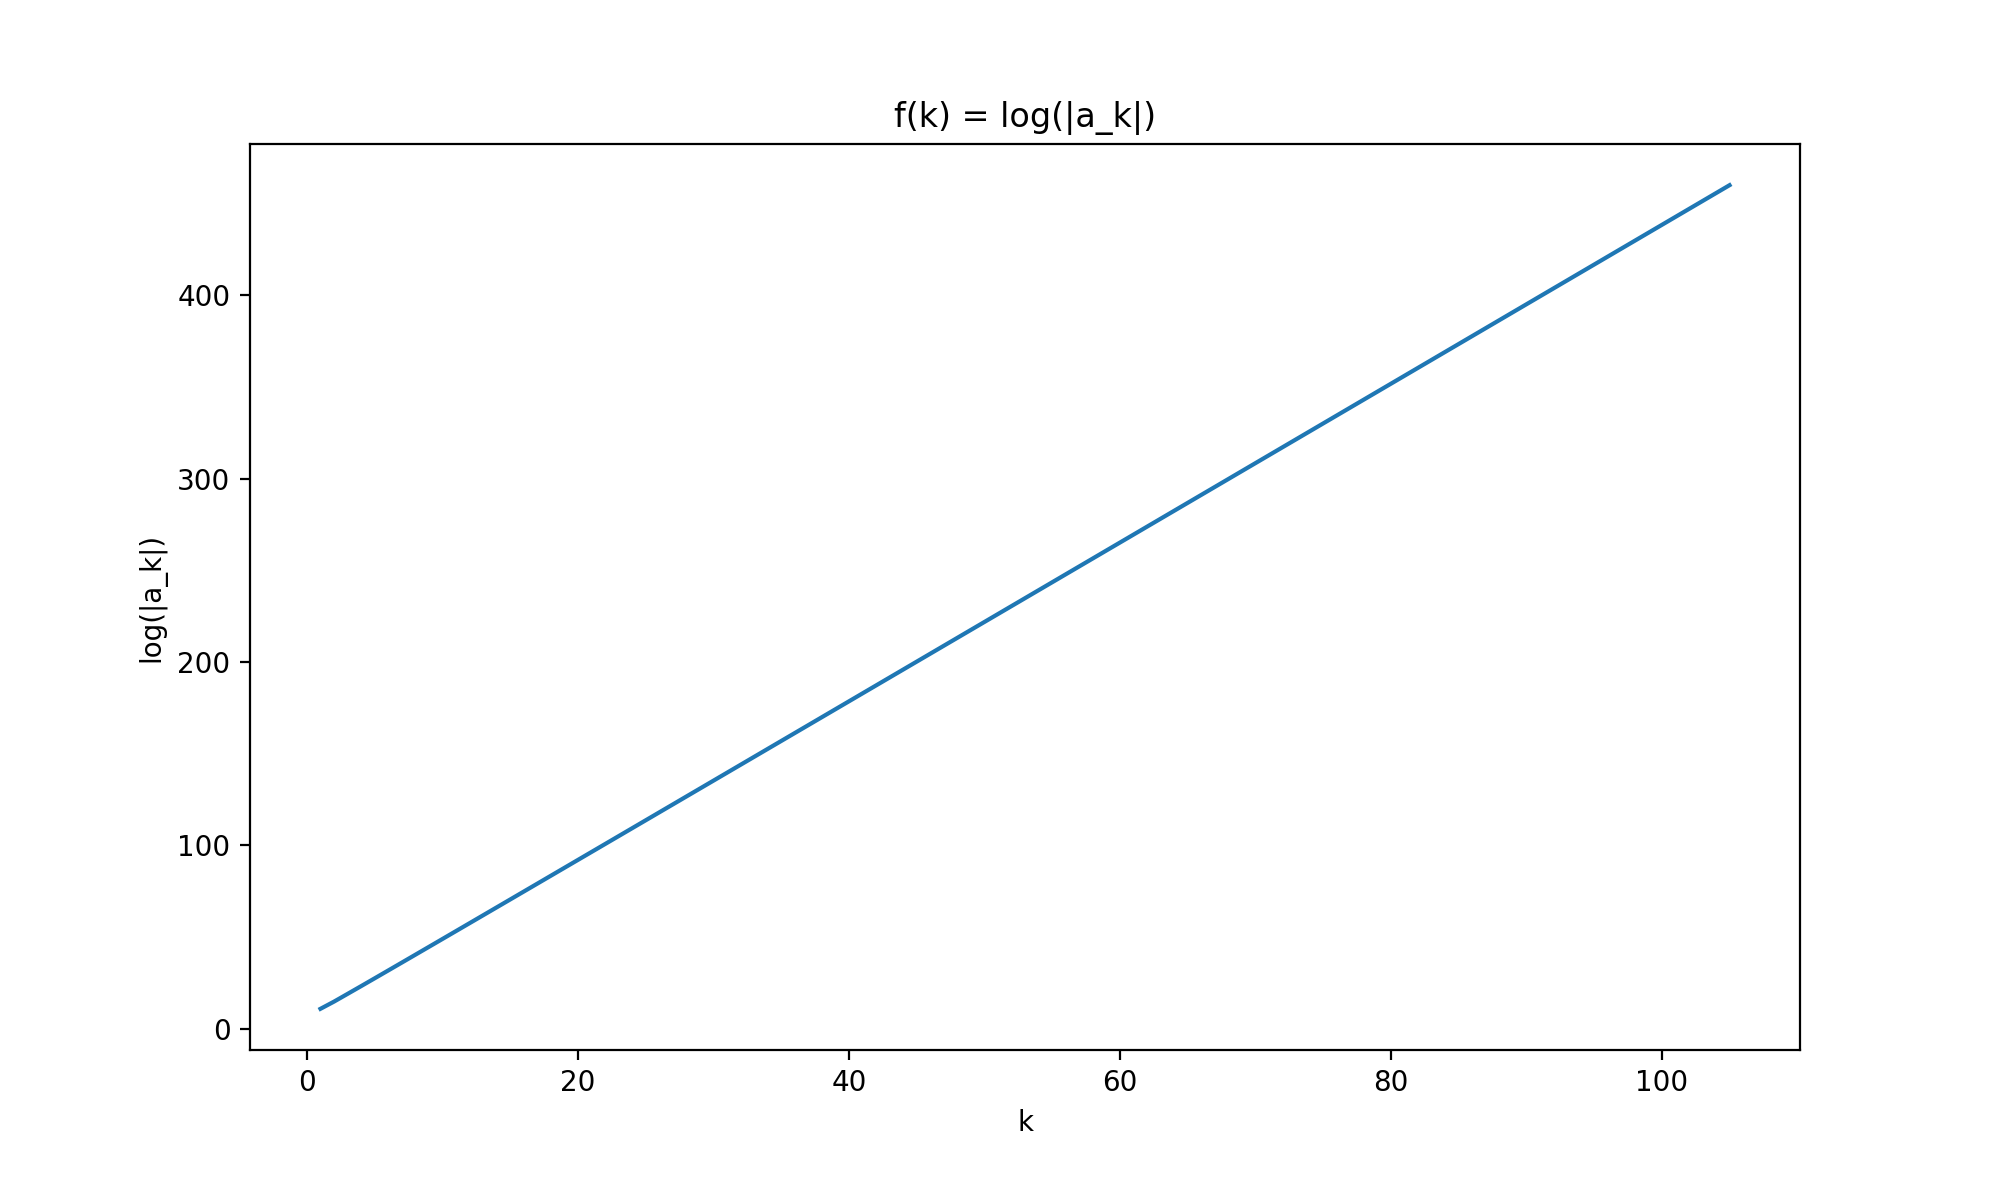
\includegraphics[width=\textwidth, height=60mm]{coefficients/logcoeff.png}
  \caption{plot of the curve $f(k) = \log(|a_k|)$, $k=0,1,\cdots,105$, confirming the exponential growth of the absolute values of the coefficients $\left\{|a_k|\right\}_{k\in\mathbb{N}} $ of $\psi(t) = \sum_{k=0}^\infty a_kt^{k\alpha}$.}
\label{barbaz}
\end{figure}
\noindent
\textbf{Step 3.}
The estimated convergence radius evaluated via \eqref{eq: estimateRadiusAnother} is $\widehat{R}_\psi = 0.00109$ (the result is rounded), computed with the knowledge of $a_{r_{max}} = a_{105} = 6.21\cdot 10^{199}$ and the formula \eqref{eq: estimateRadiusAnother}:

$$\widehat{R}_\psi = |a'_{r_{max}}|^ {-\frac{1}{\alpha r_{max}}} = |a'_{105}|^ {-\frac{1}{\alpha \cdot 105}}  = 0.00109,$$
\noindent
where we used the formula \eqref{eq: aprimo_R_radius_convergence} that gives us the relationship between the coefficients $\left\{ a'_r\right\}_{r\in \mathbb{N}}$ and $\left\{ a_r\right\}_{r\in \mathbb{N}}$.

\noindent
Note that $\widehat{R}_\psi < \frac{1}{252}= T \approx 0.004$, so that $$\theta \widehat{R}_\psi = 0.9 \widehat{R}_\psi <\frac{1}{252}=T.$$ 
Thus we will use the hybrid approach, as $T$ does not belong to the domain of absolute convergence of the fractional power series: the fractional power series is used up to $\theta \widehat{R}_\psi$, after which the Euler scheme is applied in order to compute the values $\bar{\psi}^n(t_k)$, $k=0,1,\cdots,n$.
\\
\\
\textbf{Step 4.}
Formula \eqref{eq: accuracyTruncation} gives us $r_0 = 102$. This means that in order to achieve an accuracy of $\epsilon_0 = 0.01$ with the fractional power series for $t\in [0,\theta \widehat{R}_\psi)$, it is enough to truncate at $a_{102}$: thus we will consider the truncated series 
\begin{equation}
\label{eq: truncated series n step4}
\psi^{tr}(t) = \sum_{k=0}^{102} a_k t^{k\alpha}. 
\end{equation} 
\\
\textbf{Step 5.}
Fix $n$ positive integer. In order to determine $\bar{\psi}^n(t)$ for any $t\in [0,T]$, is necessary and sufficient to determine the values $\bar{\psi}^n(t_k)$ for $k=1,\cdots ,n$ ($t_k$ and $k_0$ defined in \eqref{eq: tk and k0}), since $\bar{\psi}^n$ is a piecewise step function.
For $ t_0, t_1, \cdots, t_{k_0}$ the fractional power series is used, i.e., we set 
$$\bar{\psi}^n(t_k) = \sum_{n=0}^{102} a_n t_k^n, \hspace{0.4cm} k=0,\cdots, k_0.$$
While for $t_{k_0+1}, \cdots, t_n$, the recurrent formula \eqref{eq: 28inthepaper} based on the Euler scheme is used. 
\\

\begin{figure}[p]
  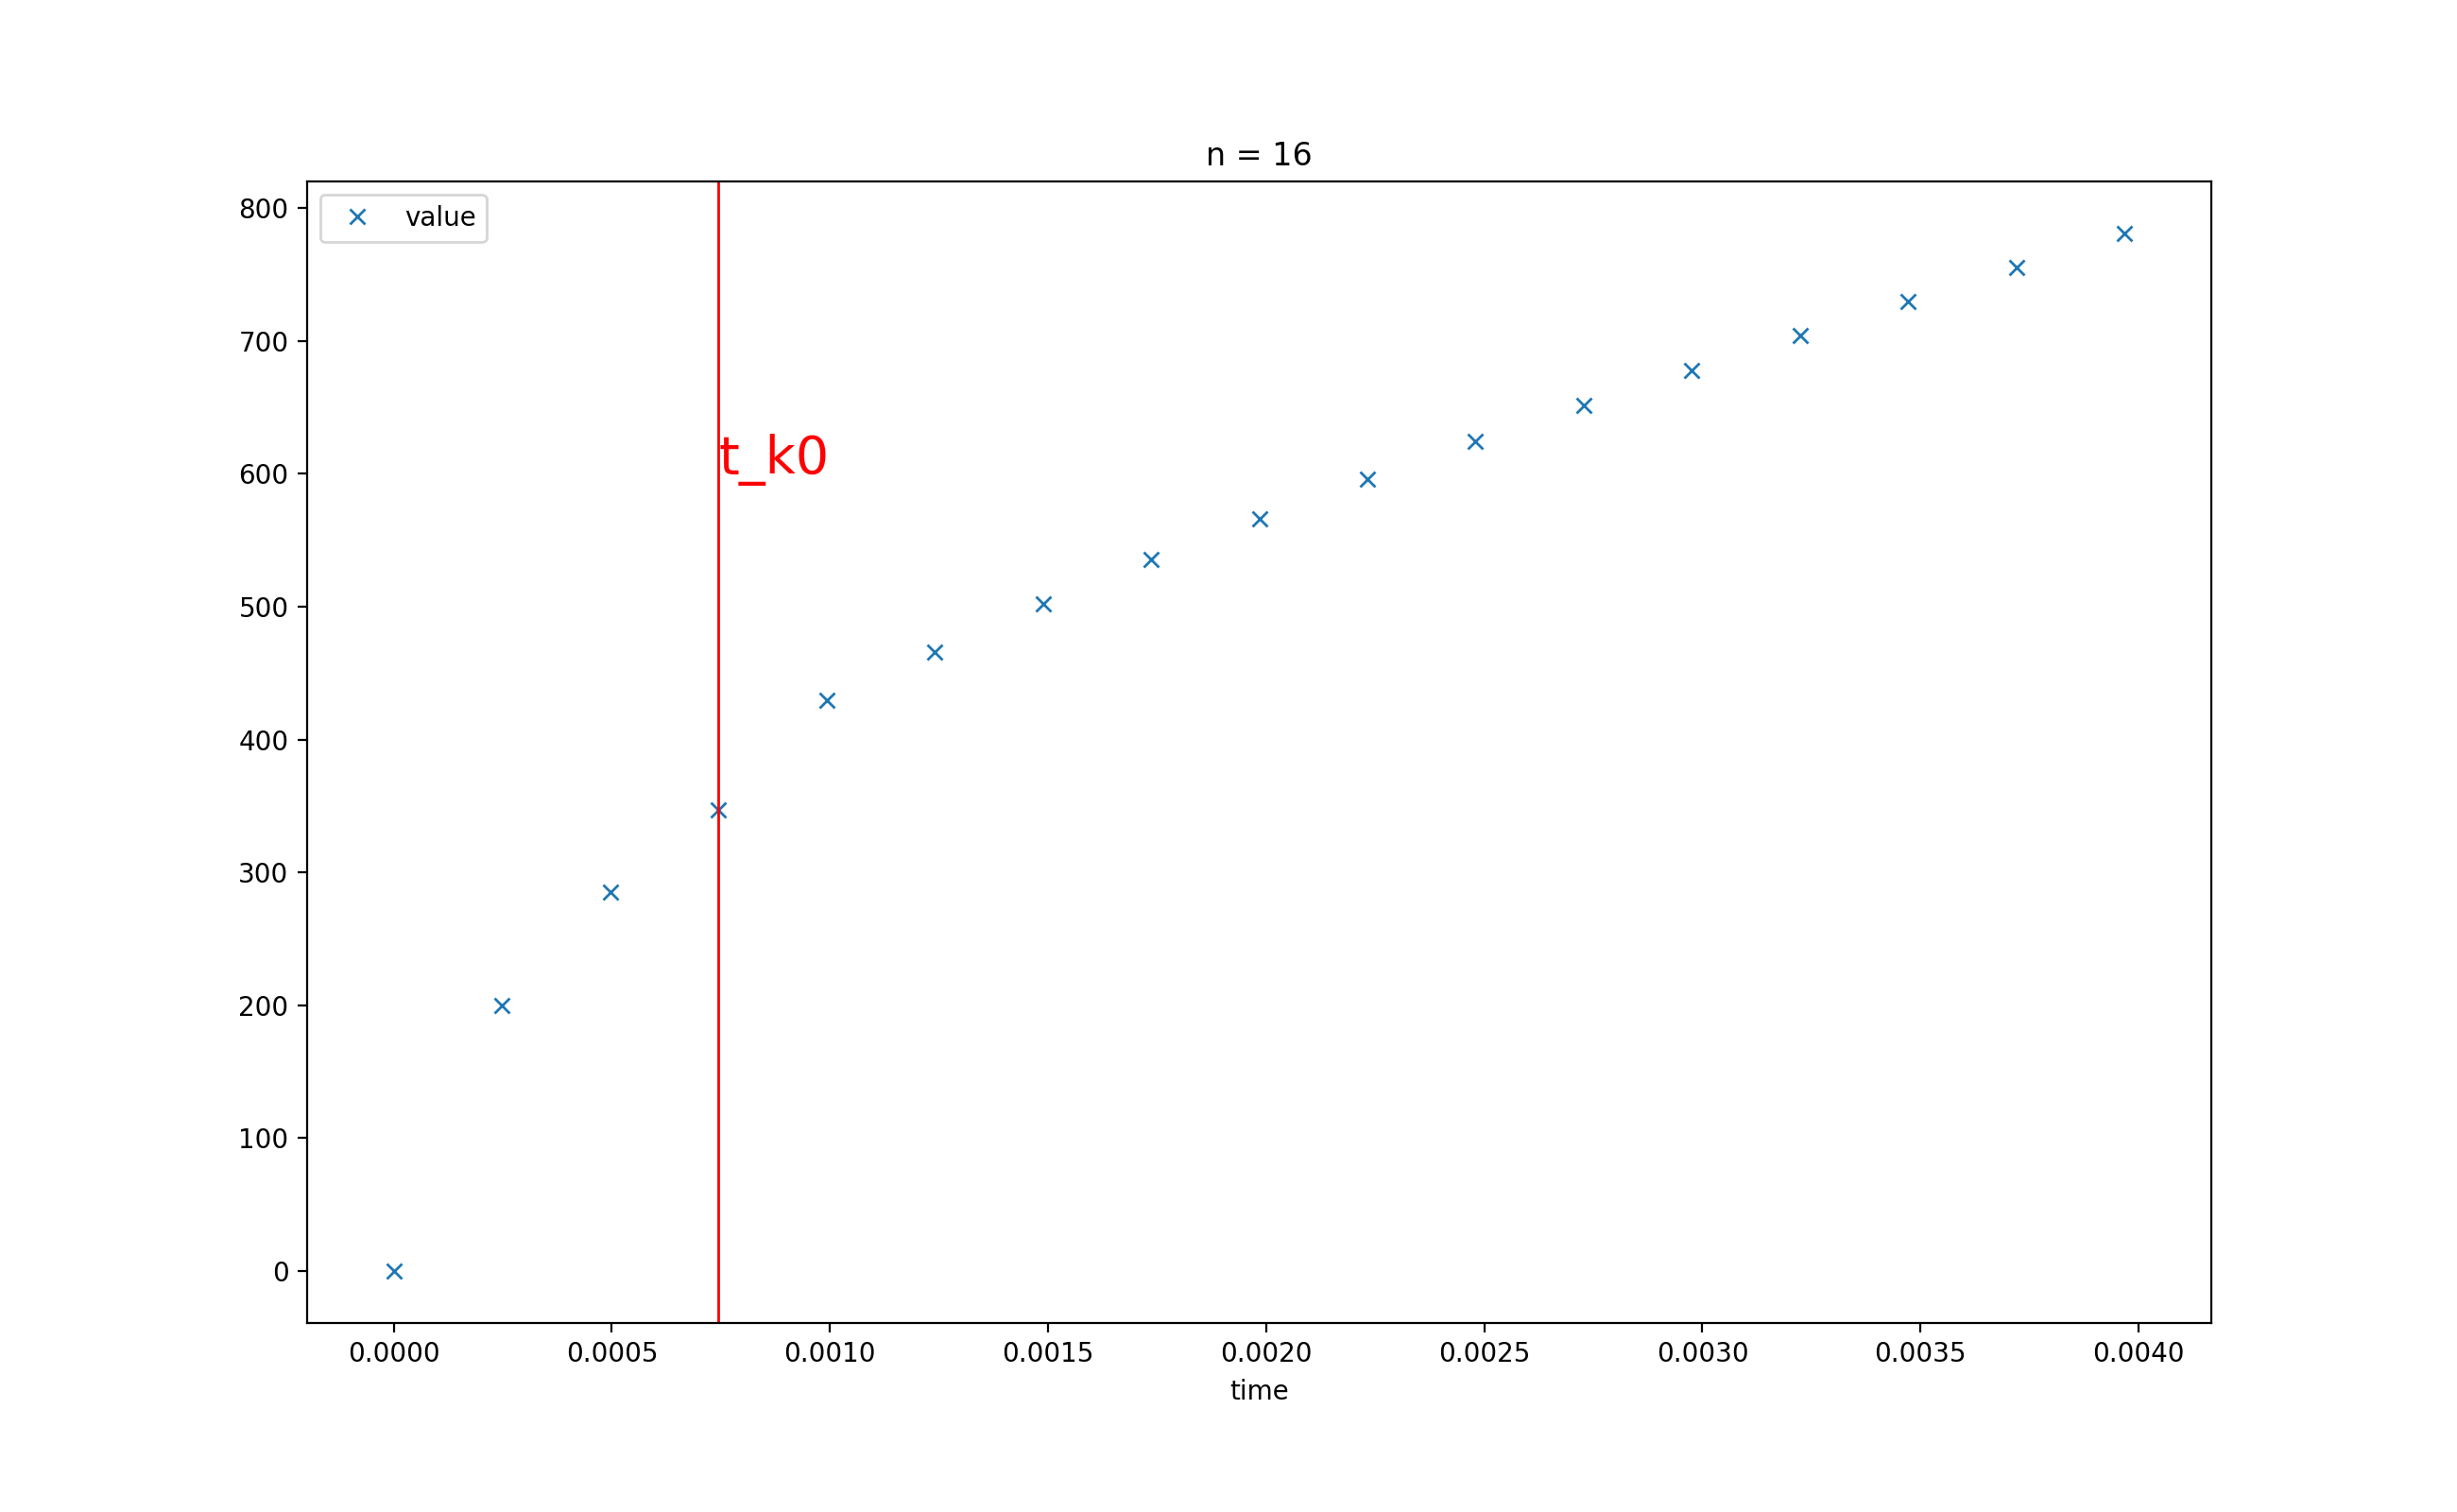
\includegraphics[width=\textwidth, height=60mm]{barpsin/n = 16.png}
  \caption{(a) curve of $\bar{\psi}^{16}(t)$ evaluated at $t=t_0,t_1,\cdots ,t_{16}$.} \label{fig: psi n=16}
\end{figure}

\begin{figure}[p]
  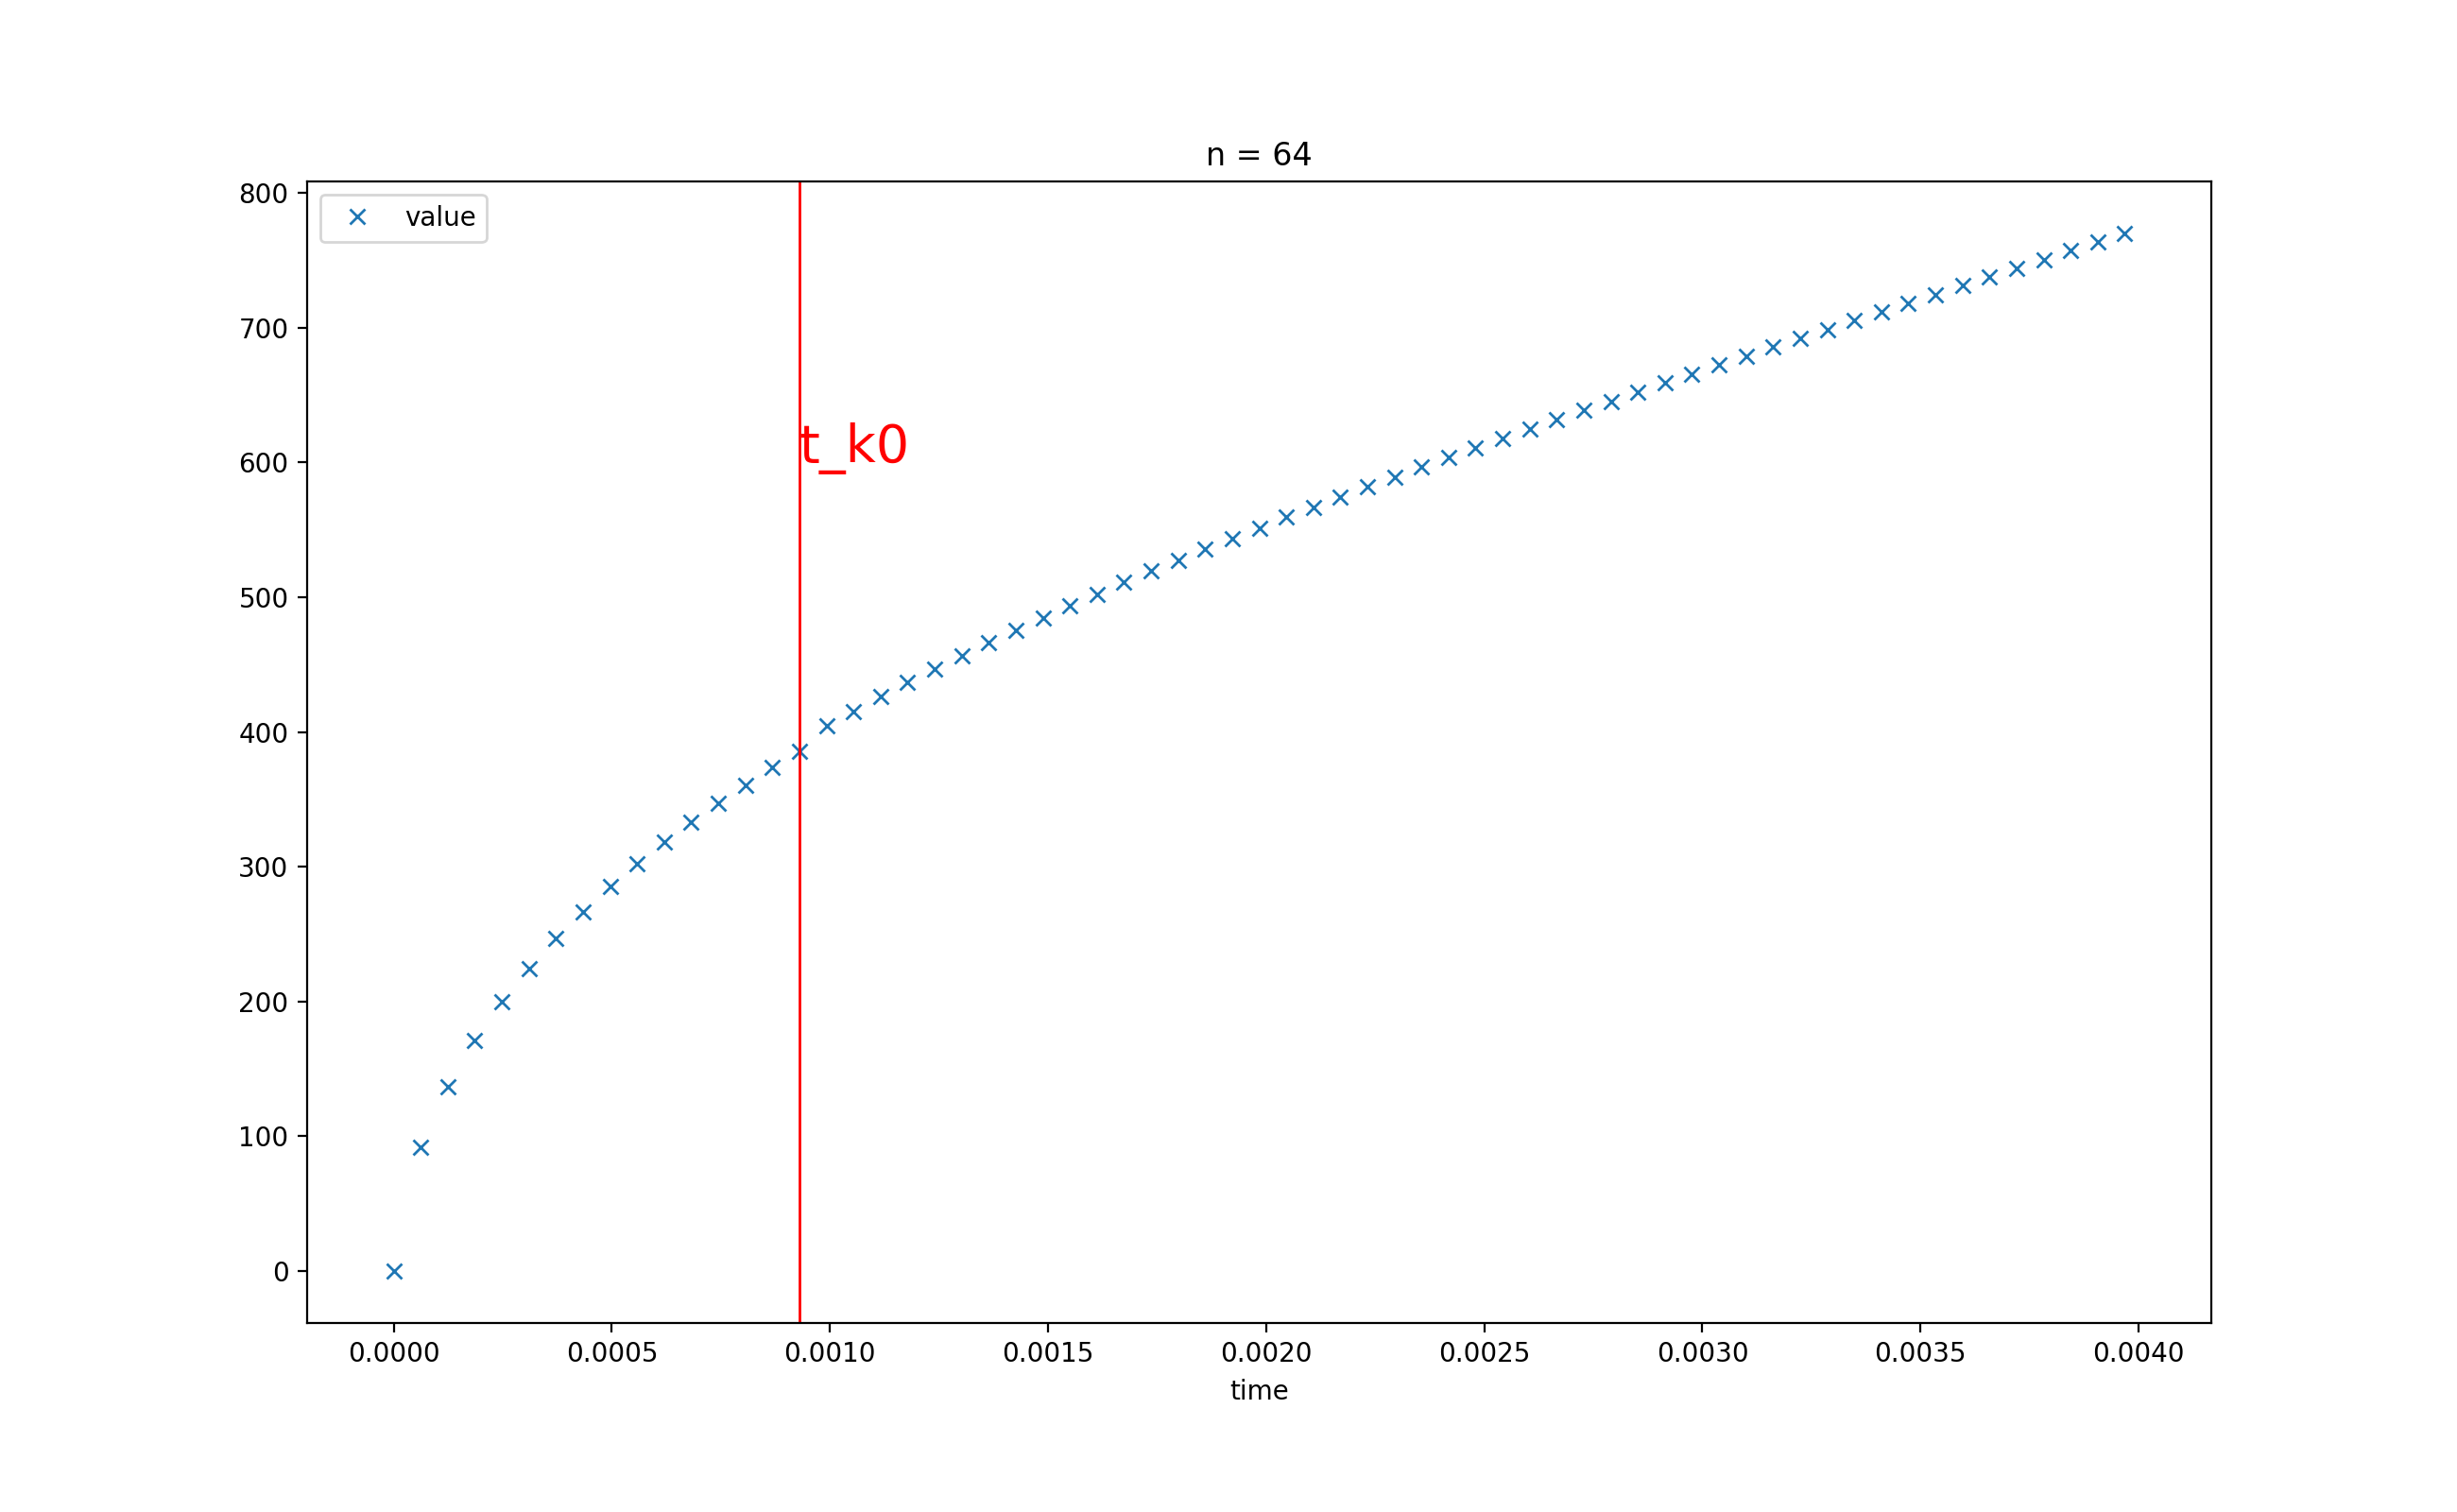
\includegraphics[width=\textwidth, height= 60mm]{barpsin/n = 64.png}
  \caption{(b) curve of $\bar{\psi}^{64}(t)$ evaluated at $t=t_0,t_1,\cdots ,t_{64}$.} \label{fig: psi n=64}
\end{figure}

\begin{figure}[p]
  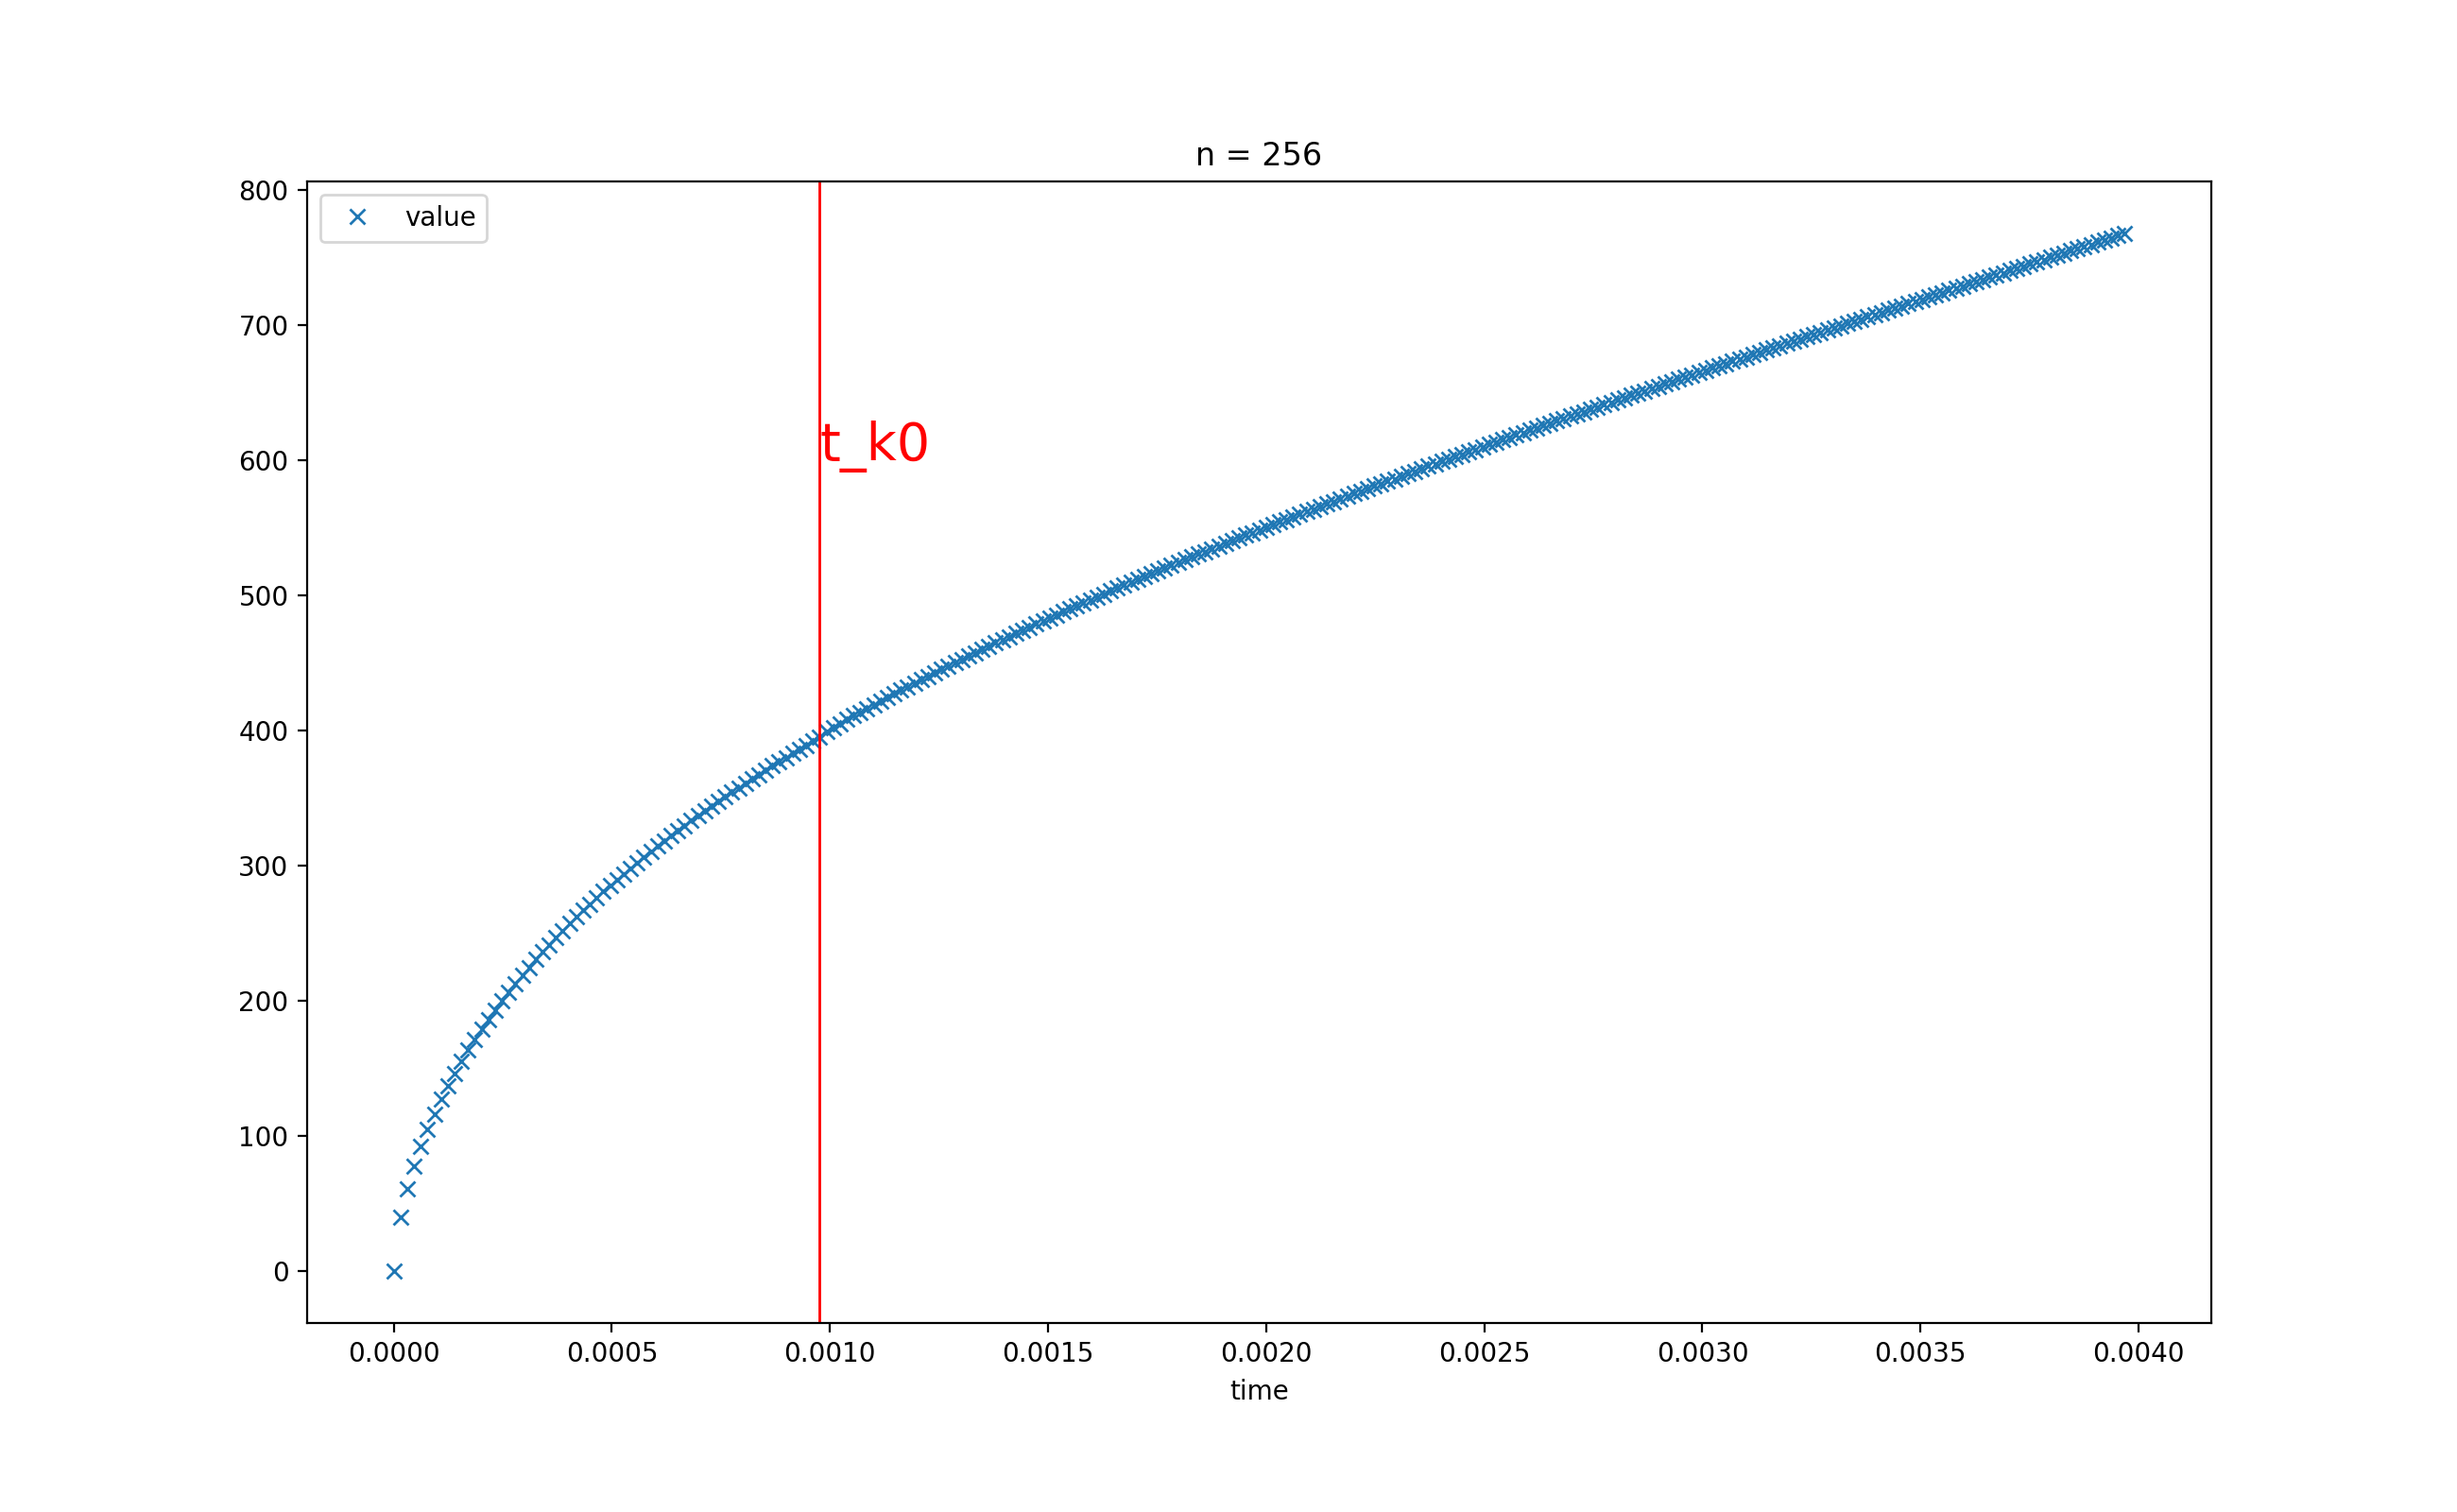
\includegraphics[width=\textwidth, height= 60mm]{barpsin/n = 256.png}
  \caption{(c) curve of $\bar{\psi}^{256}(t)$ evaluated at $t=t_0,t_1,\cdots ,t_{256}$.} \label{fig: psi n=256}
\end{figure}


In Figure \ref{fig: psi n=16}, \ref{fig: psi n=64} and \ref{fig: psi n=256} we display some plots of $\bar{\psi}^n$ for different values of $n$ ($n=16,64,256$, respectively). In these plots each point represents the value of $\bar{\psi}^n(t_l)$ for $l\in \left\{ 1,2,\cdots, n\right\}$. The red line is the value of $t_{k_0}$, which is the threshold that separates the methods we applied in order to compute the values of $\bar{\psi}^n(t_l)$, $l\in \left\{ 1,2,\cdots, n\right\}$: the fractional power series is applied with the points on the left-side of the threshold $t_{k_0}$ (i.e., for $t_0, t_1 \cdots, t_{k_0}$), and the Euler scheme with those on the right-side (i.e., for $t_{k_0+1}, \cdots, t_n$).
\\
Notice that the transition from the evaluation of the power series to the Euler scheme is ``smooth", even though we applied two different techniques. This suggests that the hybrid approach is consistent. 

Moreover, notice that the shape of the curve is robust, as it is already evident since $n=16$. Taking larger values of $n$ does not change the shape, but only contributes to have a more ``continuous" function.
\\

Up to $n=4096$, the computation times were quite reasonable, being under $1$ minute\footnote{We remind we used a computer with the following properties: 12 CPUs i7-8750H  @ 2.20GHz.} the evaluation of each $\bar{\psi}^n$.



\subsection{Computational Optimization and Observations.}
As suggested in \cite{Main}, instead of solving for the Riccati differential equation $\mathcal{E}^0_{\lambda, \mu, \nu}$ (eq. \eqref{eq: fractionalRiccati}), we can solve for $\mathcal{E}^0_{1, \mu, \nu \lambda}$ if $\lambda\ne 0$, 
being faster from the computational point of view and equivalent to the original modulo scalar non-null multiplications. 
More precisely, we have the following Lemma:
\begin{lemma}
\label{lemma: easier mult r}
Let $\phi$ be a solution to the Riccati differential equation $\mathcal{E}^0_{1, \mu, \nu \lambda}$ (eq. \eqref{eq: fractionalRiccati}) and $\lambda \ne 0$.
Then $\psi := \frac{\phi}{\lambda}$ is a solution to $\mathcal{E}^0_{\lambda, \mu, \nu}$.
\end{lemma}
\begin{proof} [Proof. of Lemma \ref{lemma: easier mult r}.] 
Let $\phi$ be a solution to $\mathcal{E}^0_{1, \mu, \nu \lambda}$. Therefore it holds
$$D^\alpha \phi = \phi^2 + \mu \phi + \nu \lambda. $$
Dividing both sides by $\lambda$ (we assumed $\lambda \ne 0)$ yields to
$$D^\alpha \left(\frac{\phi}{\lambda} \right) = \lambda \left(\frac{\phi}{\lambda}\right)^2 + \mu \frac{\phi}{\lambda} + \nu,$$
\noindent
so that defining $\psi := \frac{\phi}{\lambda}$ follows that $\psi$ is a solution to $\mathcal{E}^0_{\lambda,\mu,\nu}$, as desired. 
\end{proof}
\\
\\
\noindent
The optimal threshold factor $\theta = \theta(n)$ (recall Subsection \ref{subsection: accuracy in truncating}) is suggested to be (see \cite{Main} for reference)
\\
$$\theta(n) := \min \left(0.65 + 0.3\left( \frac{n-32}{4064} \right)^{0.25}, 0.925\right) $$
\\
\noindent
for $32 \le n \le 4096$.
Notice that the function $\theta(n)$ defined above is increasing, reaching a maximum of $0.925$. 
However, for values of $n\approx 2000$ we already have $\theta(n) \approx 0.9$, and preferably we would like to have greater values of $n$ for a better accuracy. Moreover, for such values of $n$ the computational cost is still very low for the machine (under one minute of computation for $\bar{\psi}^n$, $n\le 4000$, in this particular test with a machine with the properties described in \eqref{eq: ref properties pc}). This is why in our experimentations we set $\theta=0.9$ fixed independent by $n$.

\section{Computing $c_1$.}
\label{section: computingc1}

In this section we continue the numerical tests, using the same parameters given in equation \eqref{eq: NumericalTestParameters} and $T=\frac{1}{252}$, with precision set to $\epsilon_0 = 0.01$. 
As discussed previously (Subsection \ref{subsection: rrfirst_estimate} and Section \ref{section: extrapolatedhyb}), if we assume the estimate \eqref{eq: 30inthepaper}, which we recall being
$$ \bar{\psi}^n(T) - \psi(T) = \frac{c_1}{n}+ o(n^{-1}) $$
for some constant $c_1 \in \mathbb{R}$, then we can use the Richardson-Romberg extrapolation. Furthermore, the constant $c_1$ can be computed as described in Remark \ref{remark: c1_series}, i.e., as limit of the sequence $\left\{ \bar{c}_1^n \right\}_{n \in \mathbb{N}}$ (as $n\to +\infty$), which we recall being defined by
$$ \bar{c}_1^n := 2n \left( \bar{\psi}^n(T) - \bar{\psi}^{2n}(T) \right). $$ 
From the previous Section (Section \ref{section: generalprocedure}), we already have the algorithm to compute $\bar{\psi}^n(T)$ for any $n$ positive integer, so that we can easily find $\bar{c}_1^n$. 
The results that we obtained are displayed in Table \ref{c1table}, where are presented the different values of $\bar{c}_1^n$ that we obtained for $n= 2^2, 2^3, \cdots, 2^{17}$. 
We also have the column with the computation time in seconds for each $\bar{c}_1^n$. 
Furthermore, there is the ratio of consecutive computation times: if we denote by $C(\bar{c}_1^n)$ the computation time in seconds required to evaluate $\bar{c}_1^n$, then the column "ratio of consecutive computation times" is $\frac{C(\bar{c}_1^n)}{C(\bar{c}_1^{n/2})}$.

\begin{table}[ht]
\centering
\begin{tabular}{ |c|c|c|c| } 
 \hline
 $n$ & $\bar{c_1}^n$ & {\footnotesize computation time (seconds)} & {\footnotesize ratio of consecutive computation times} \\ 
 \hline
 4 & 244.789055 & 0.005540 & - \\ 
 \hline
 8 & 247.620217  & 0.005834 & 1.053153 \\
 \hline
 16 & 236.228489 & 0.004871 & 0.834941 \\
 \hline
 32 & 224.837873 &  0.005614 & 1.152562 \\
 \hline
 64 & 215.948954 & 0.009873 & 1.758578  \\
 \hline
 128 & 209.595284 & 0.018452 & 1.868924\\
 \hline
 256 & 205.598250 & 0.059347 & 3.216283\\
 \hline
 512 & 202.148404 & 0.221983 & 3.740396 \\
 \hline
 1024 & 199.883079 & 0.862326 & 3.884654 \\
 \hline
 2048 & 198.677258 & 3.469351 & 4.023247 \\
 \hline
 4096 & 197.780231 & 14.281353 & 4.116433 \\
 \hline
 8192 & 197.255466 & 57.106588 & 3.998682 \\
 \hline
 16384 & 196.916654 & 227.248170 & 3.979369 \\
 \hline
 32768 & 196.699728 & 926.553653 &  4.077277\\
 \hline
 65536 & 196.555097 & 3687.706343 & 3.980025\\
 \hline
 131072 & 196.510382 & 14858.320412 & 4.029150 \\
 \hline
\end{tabular}
\caption{evaluations of $\bar{c_1}^n$ (defined in equation \eqref{eq: 32inthepaper}) and computation times.}
\label{c1table}
\end{table}

%\begin{figure}[H]
%  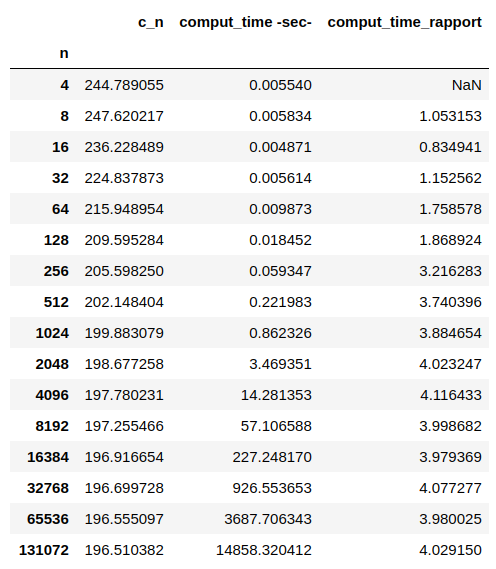
\includegraphics[width=11.5cm]{c1n/c_11table.png}
%  \caption{$\bar{c}_1^n table $}\label{c1table}
%\end{figure}

It seems that the sequence $\left\{ \bar{c}_1^n\right\}_{n\in \mathbb{N}}$ converges (see also Figure \ref{c1plot1}), suggesting that the estimate \eqref{eq: 30inthepaper} holds.  We take as reference limit the value 
\begin{equation}
\label{eq: c1maxref}
 c_1^{ref} :=\bar{c}_1^{n_{max}} = 196.510382,
\end{equation}  where $n_{max} = 2^{17}=131072$.
\\

In the next Subsection \ref{subsection: plots and confirm rr estimate} we will see some more plots that will test the validity of the two estimates \eqref{eq: 30inthepaper} and \eqref{eq: moreAccurateEstimate}, which we remind being, respectively, $$\bar{\psi}^n(T)-\psi(T) = \frac{c_1}{n} + o(n^{-1})$$ for a constant $c_1\in \mathbb{R}$ and $$\bar{\psi}^n(T)-\psi(T) = \frac{c_1}{n} + \frac{c_2}{n^2} + o(n^{-2})$$ for some constants $c_1, c_2\in \mathbb{R}$. We will refer to them as the RR estimates (first and second order respectively), since they allow us to perform the Richardson-Romberg extrapolation (single and double step, respectively).

\subsection{Plots and validation of the RR estimates.}
\label{subsection: plots and confirm rr estimate}

Figure \ref{c1plot1} and \ref{c1plot1v2} show $\bar{c_1}^n$ as a function of $n$ (for numerical values see Table \ref{c1table}).

\begin{figure}[ht]
  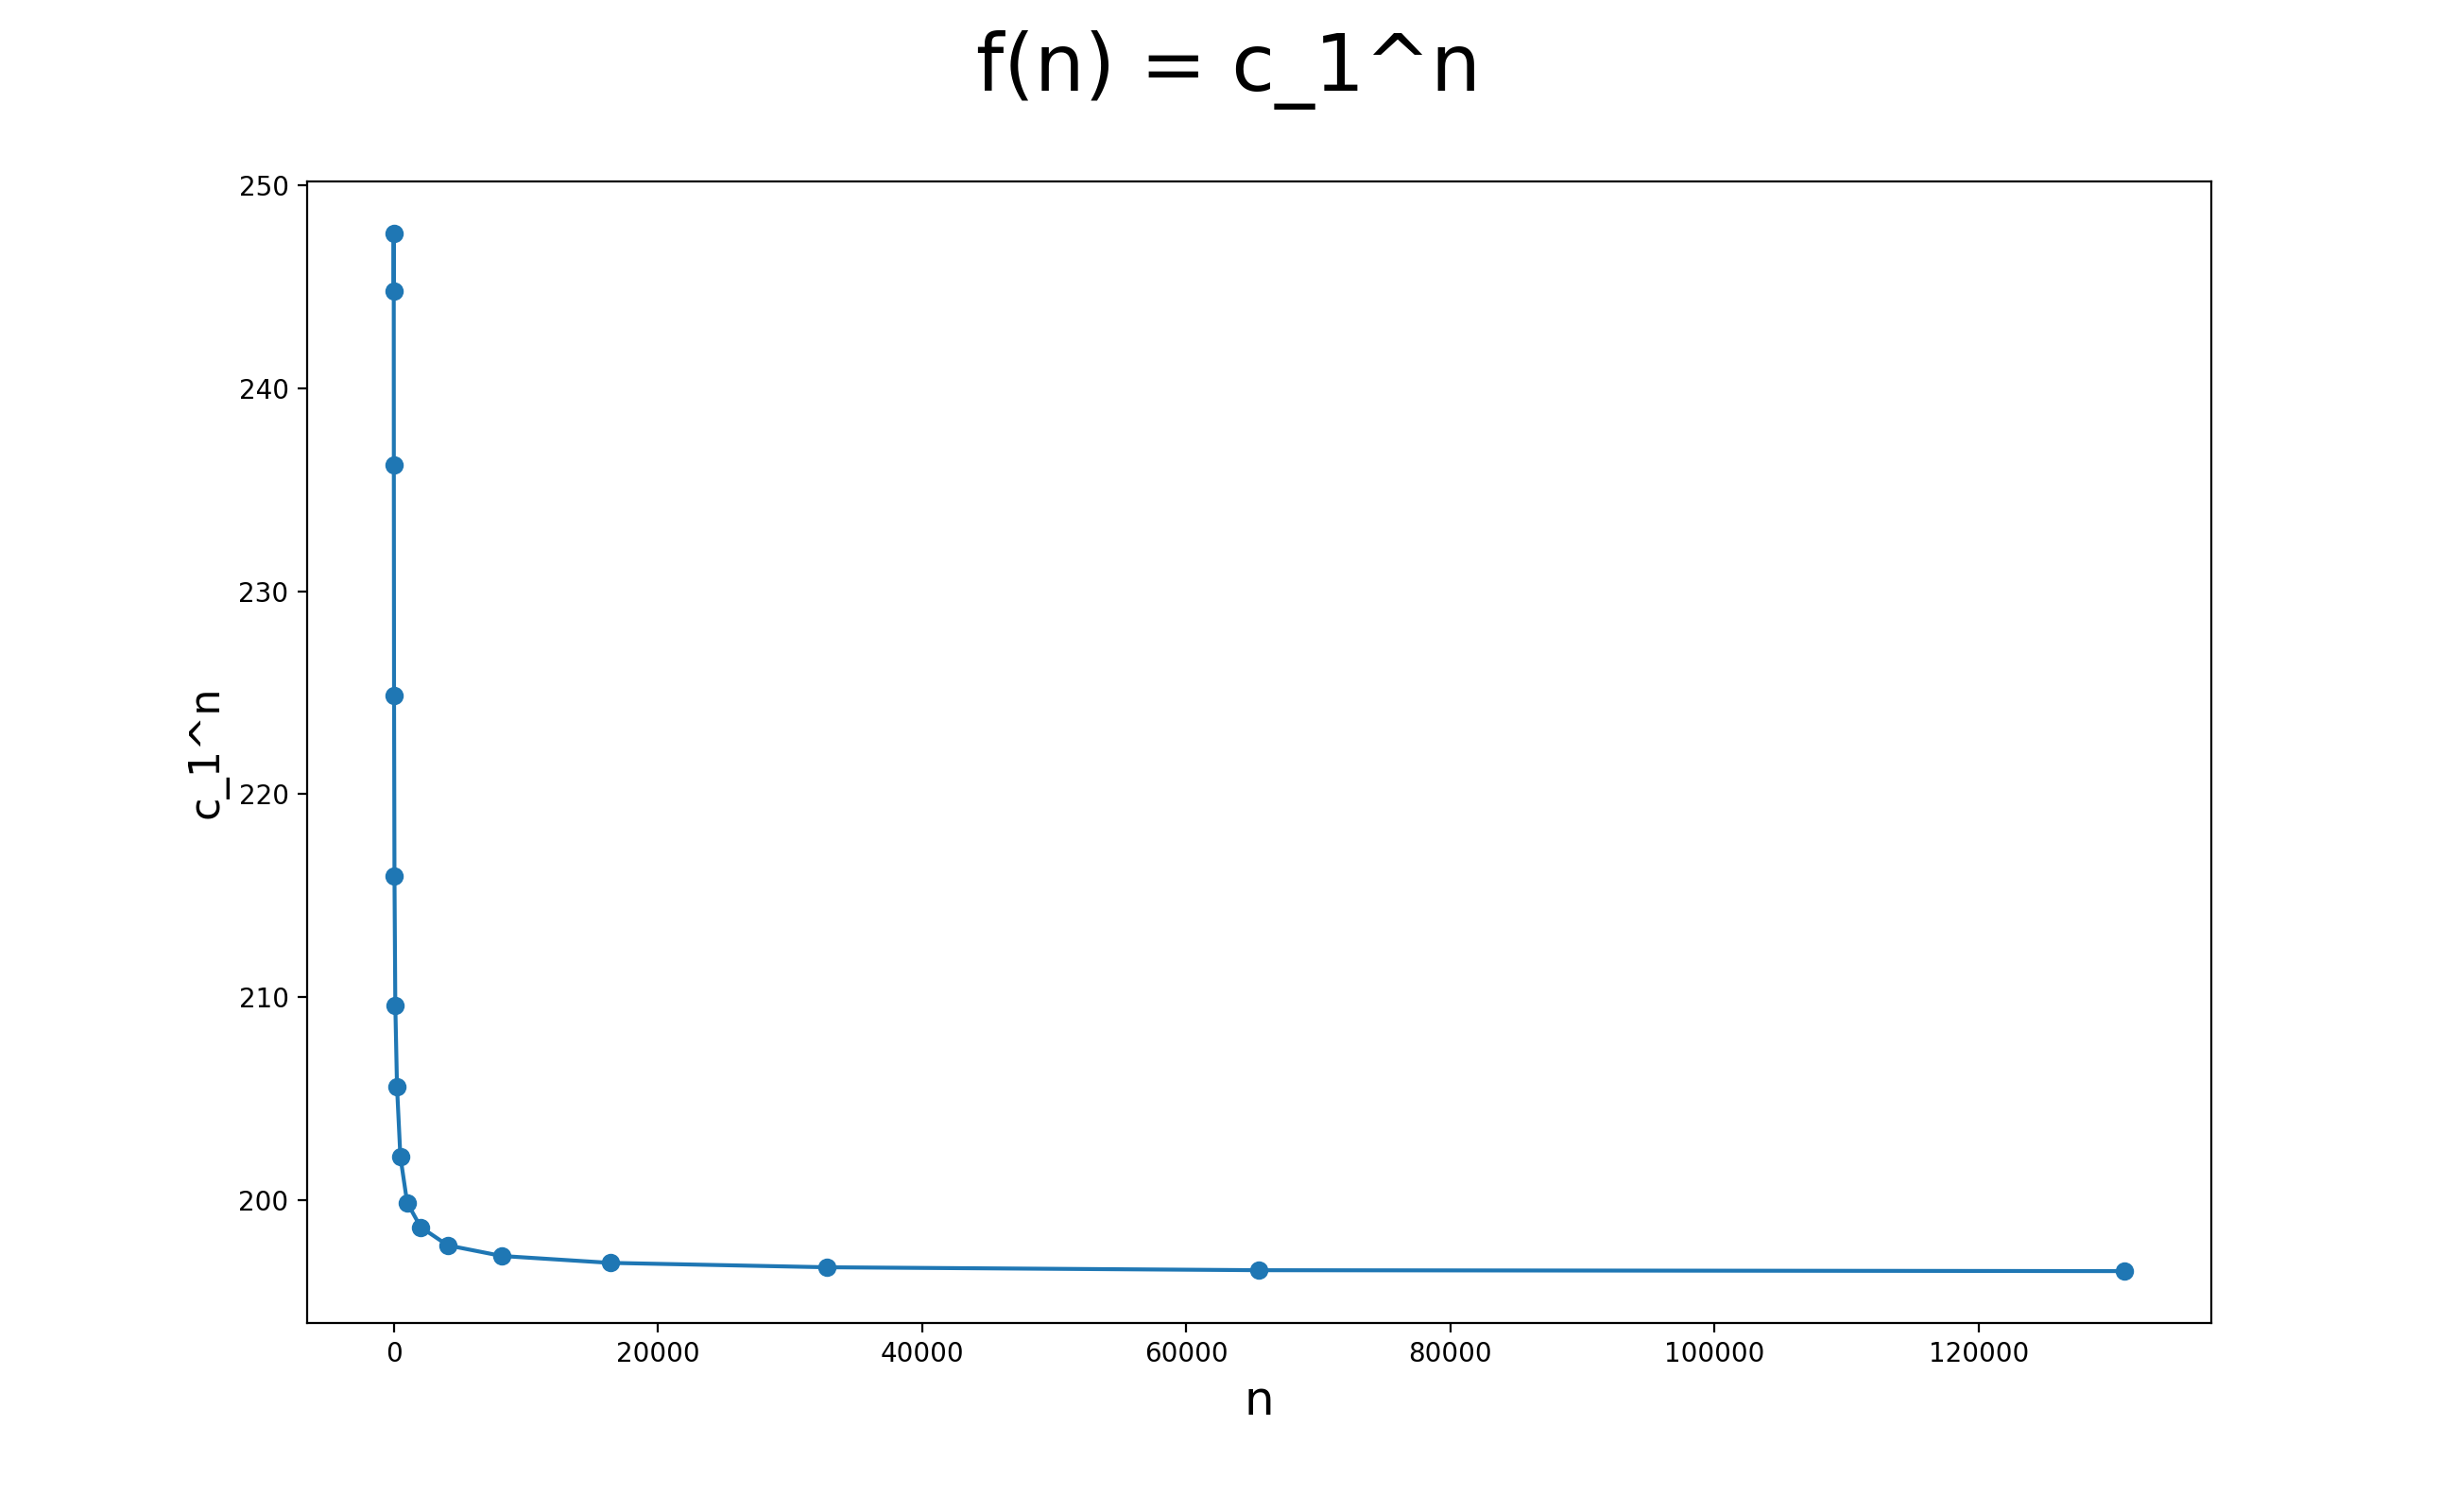
\includegraphics[width=\textwidth, height=55mm]{c1n/c_1^n.png}
  \caption{we plot $\bar{c}_1^n$ as a function of $n$: $f(n):=\bar{c}_1^n $.}\label{c1plot1}
\end{figure}

\begin{figure}[ht]
  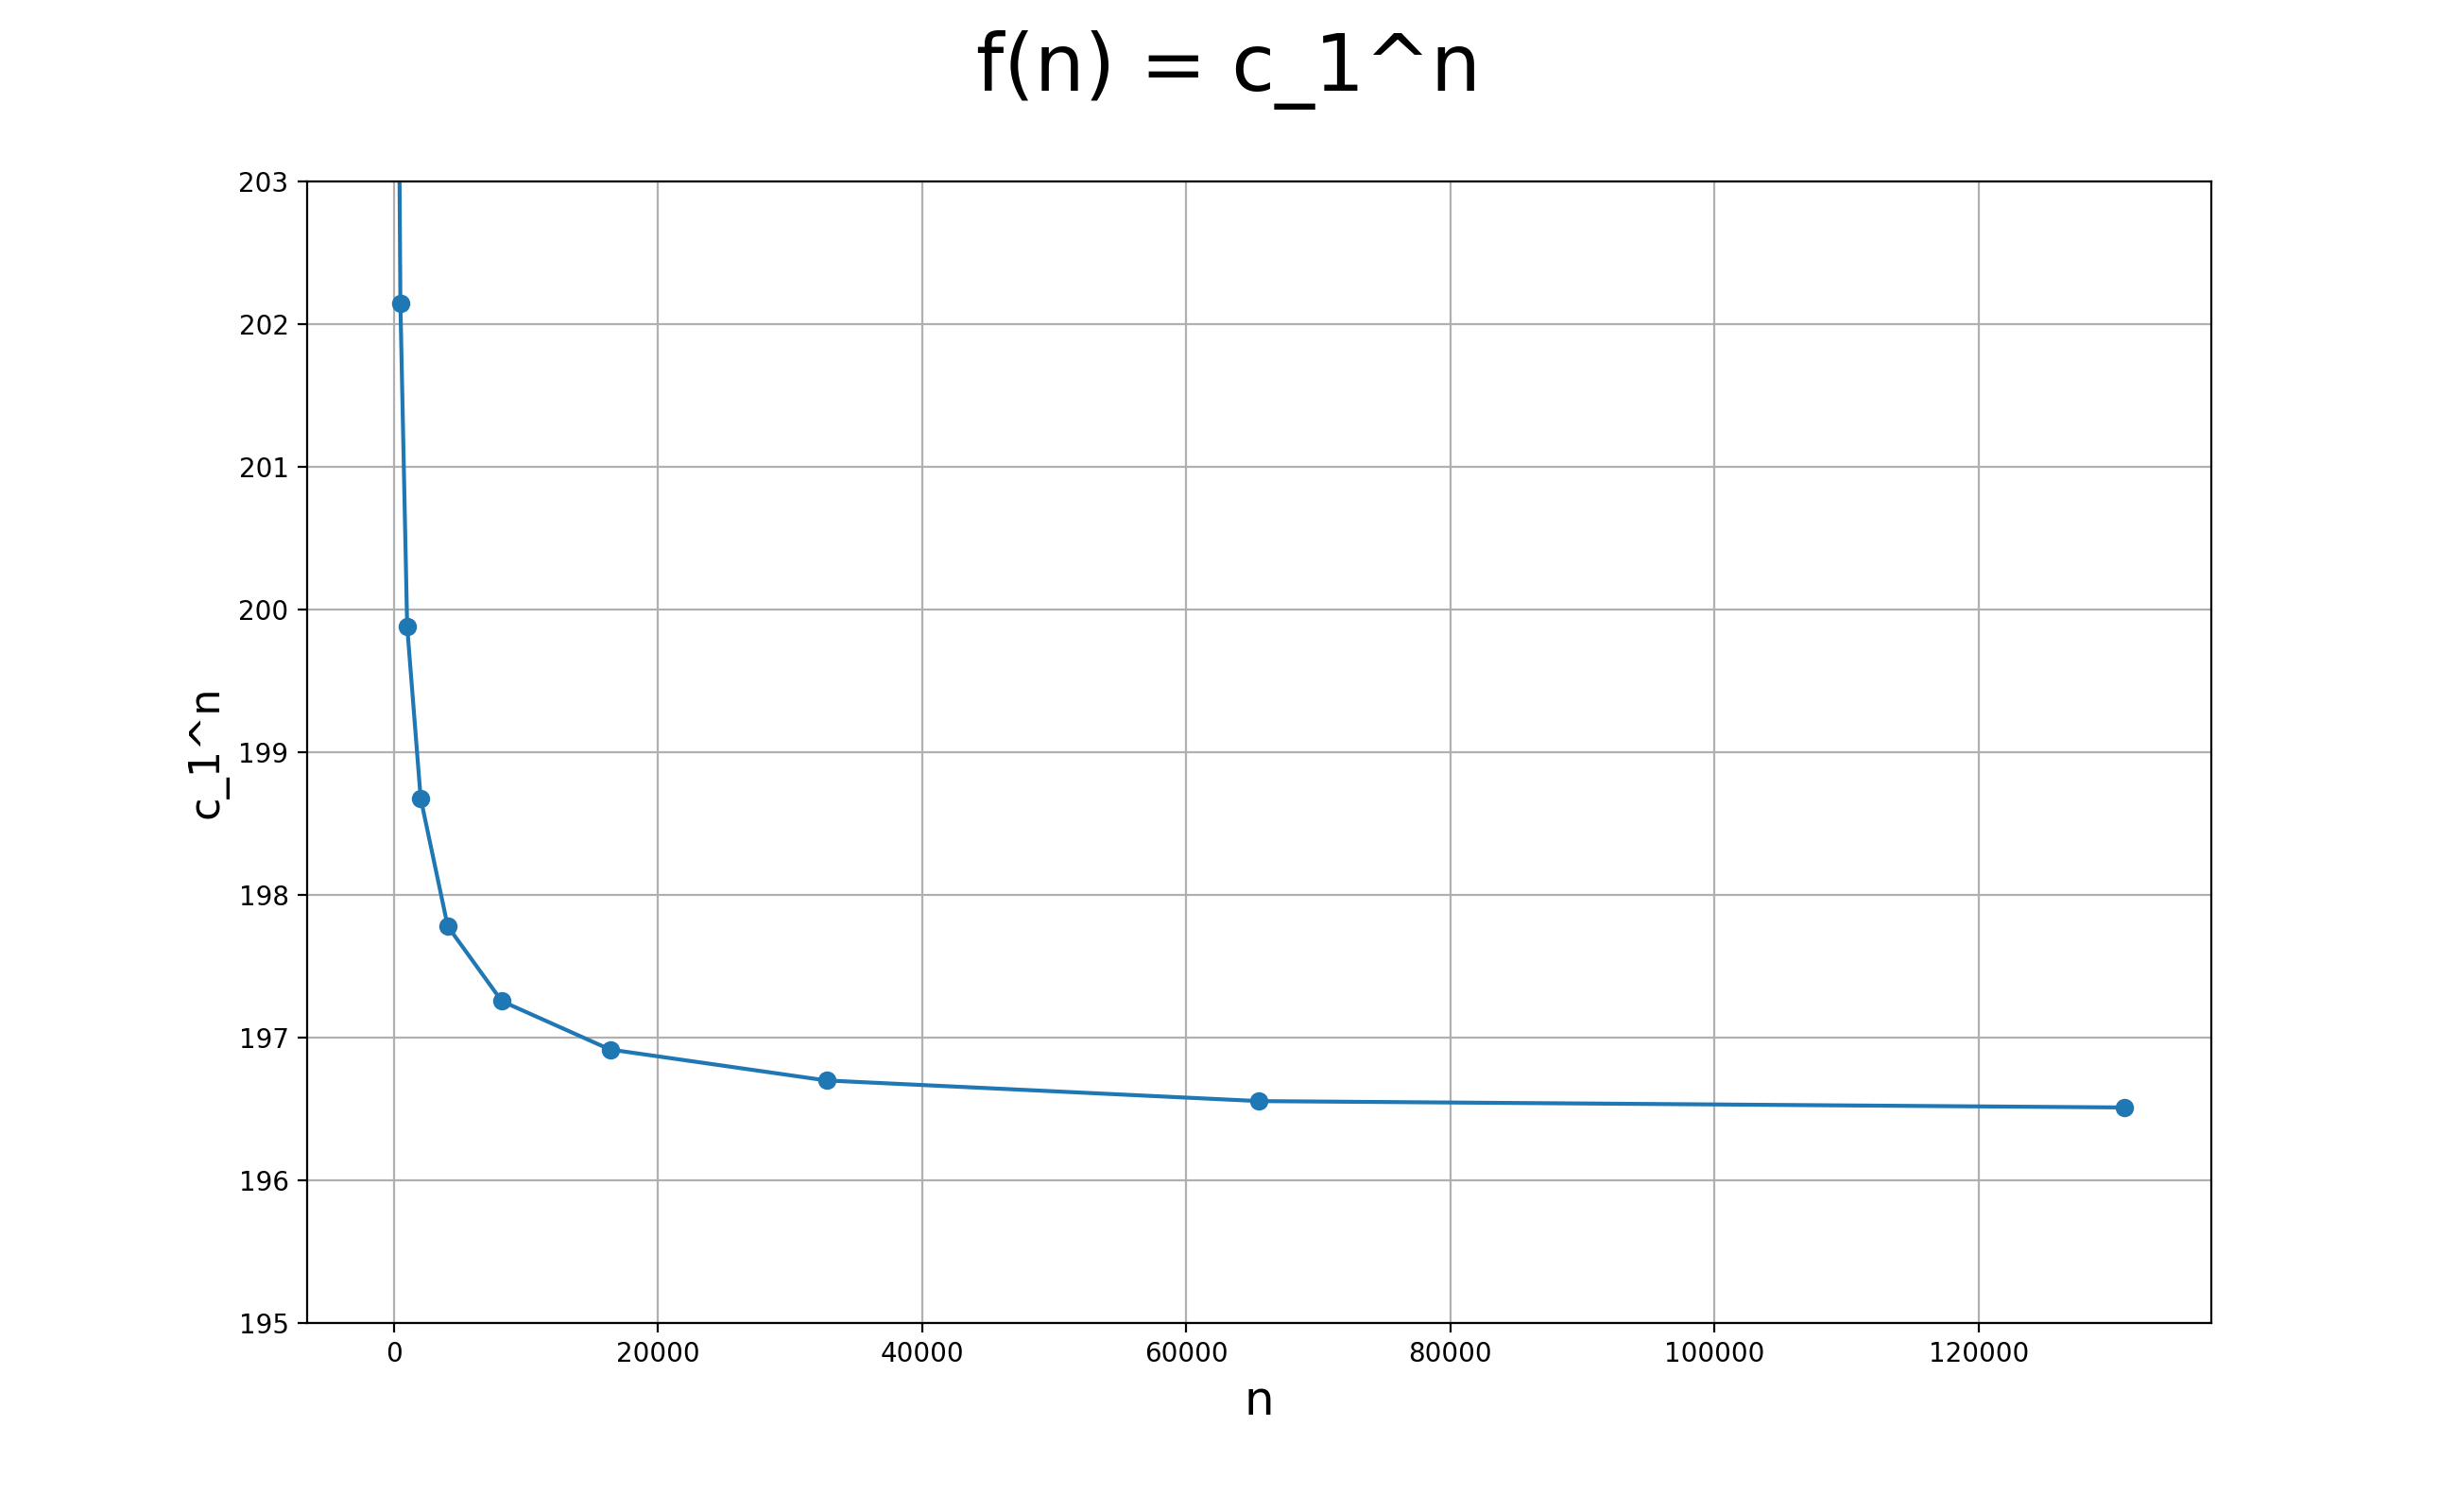
\includegraphics[width=\textwidth, height=55mm]{c1n/c_1^n_zoomed.png}
  \caption{the same plot as Figure \ref{c1plot1} ($\bar{c}_1^n$ as a function of $n$: $f(n):=\bar{c}_1^n$) but zoomed on the $y$-axis.}\label{c1plot1v2}
\end{figure}


From the plot in Figure \ref{c1plot1} (and \ref{c1plot1v2}) it is more evident that the sequence $\left\{\bar{c}_1^n \right\}_{n\in\mathbb{N}}$ converges.
If the RR estimate \eqref{eq: 30inthepaper} holds, then a necessary condition is that $$\lim_{n\to +\infty}\bar{c_1}^n  = c_1,$$ as shown in \eqref{eq: 32inthepaper}. 
However, this is not a sufficient condition for the RR estimate to hold.
\\

Now, the plot in Figure \ref{c1plotlog} shows  $\log(\bar{c_1}^n-\bar{c_1}^{ref})$ as a function of $\log(n)$.

\begin{figure}[ht]
  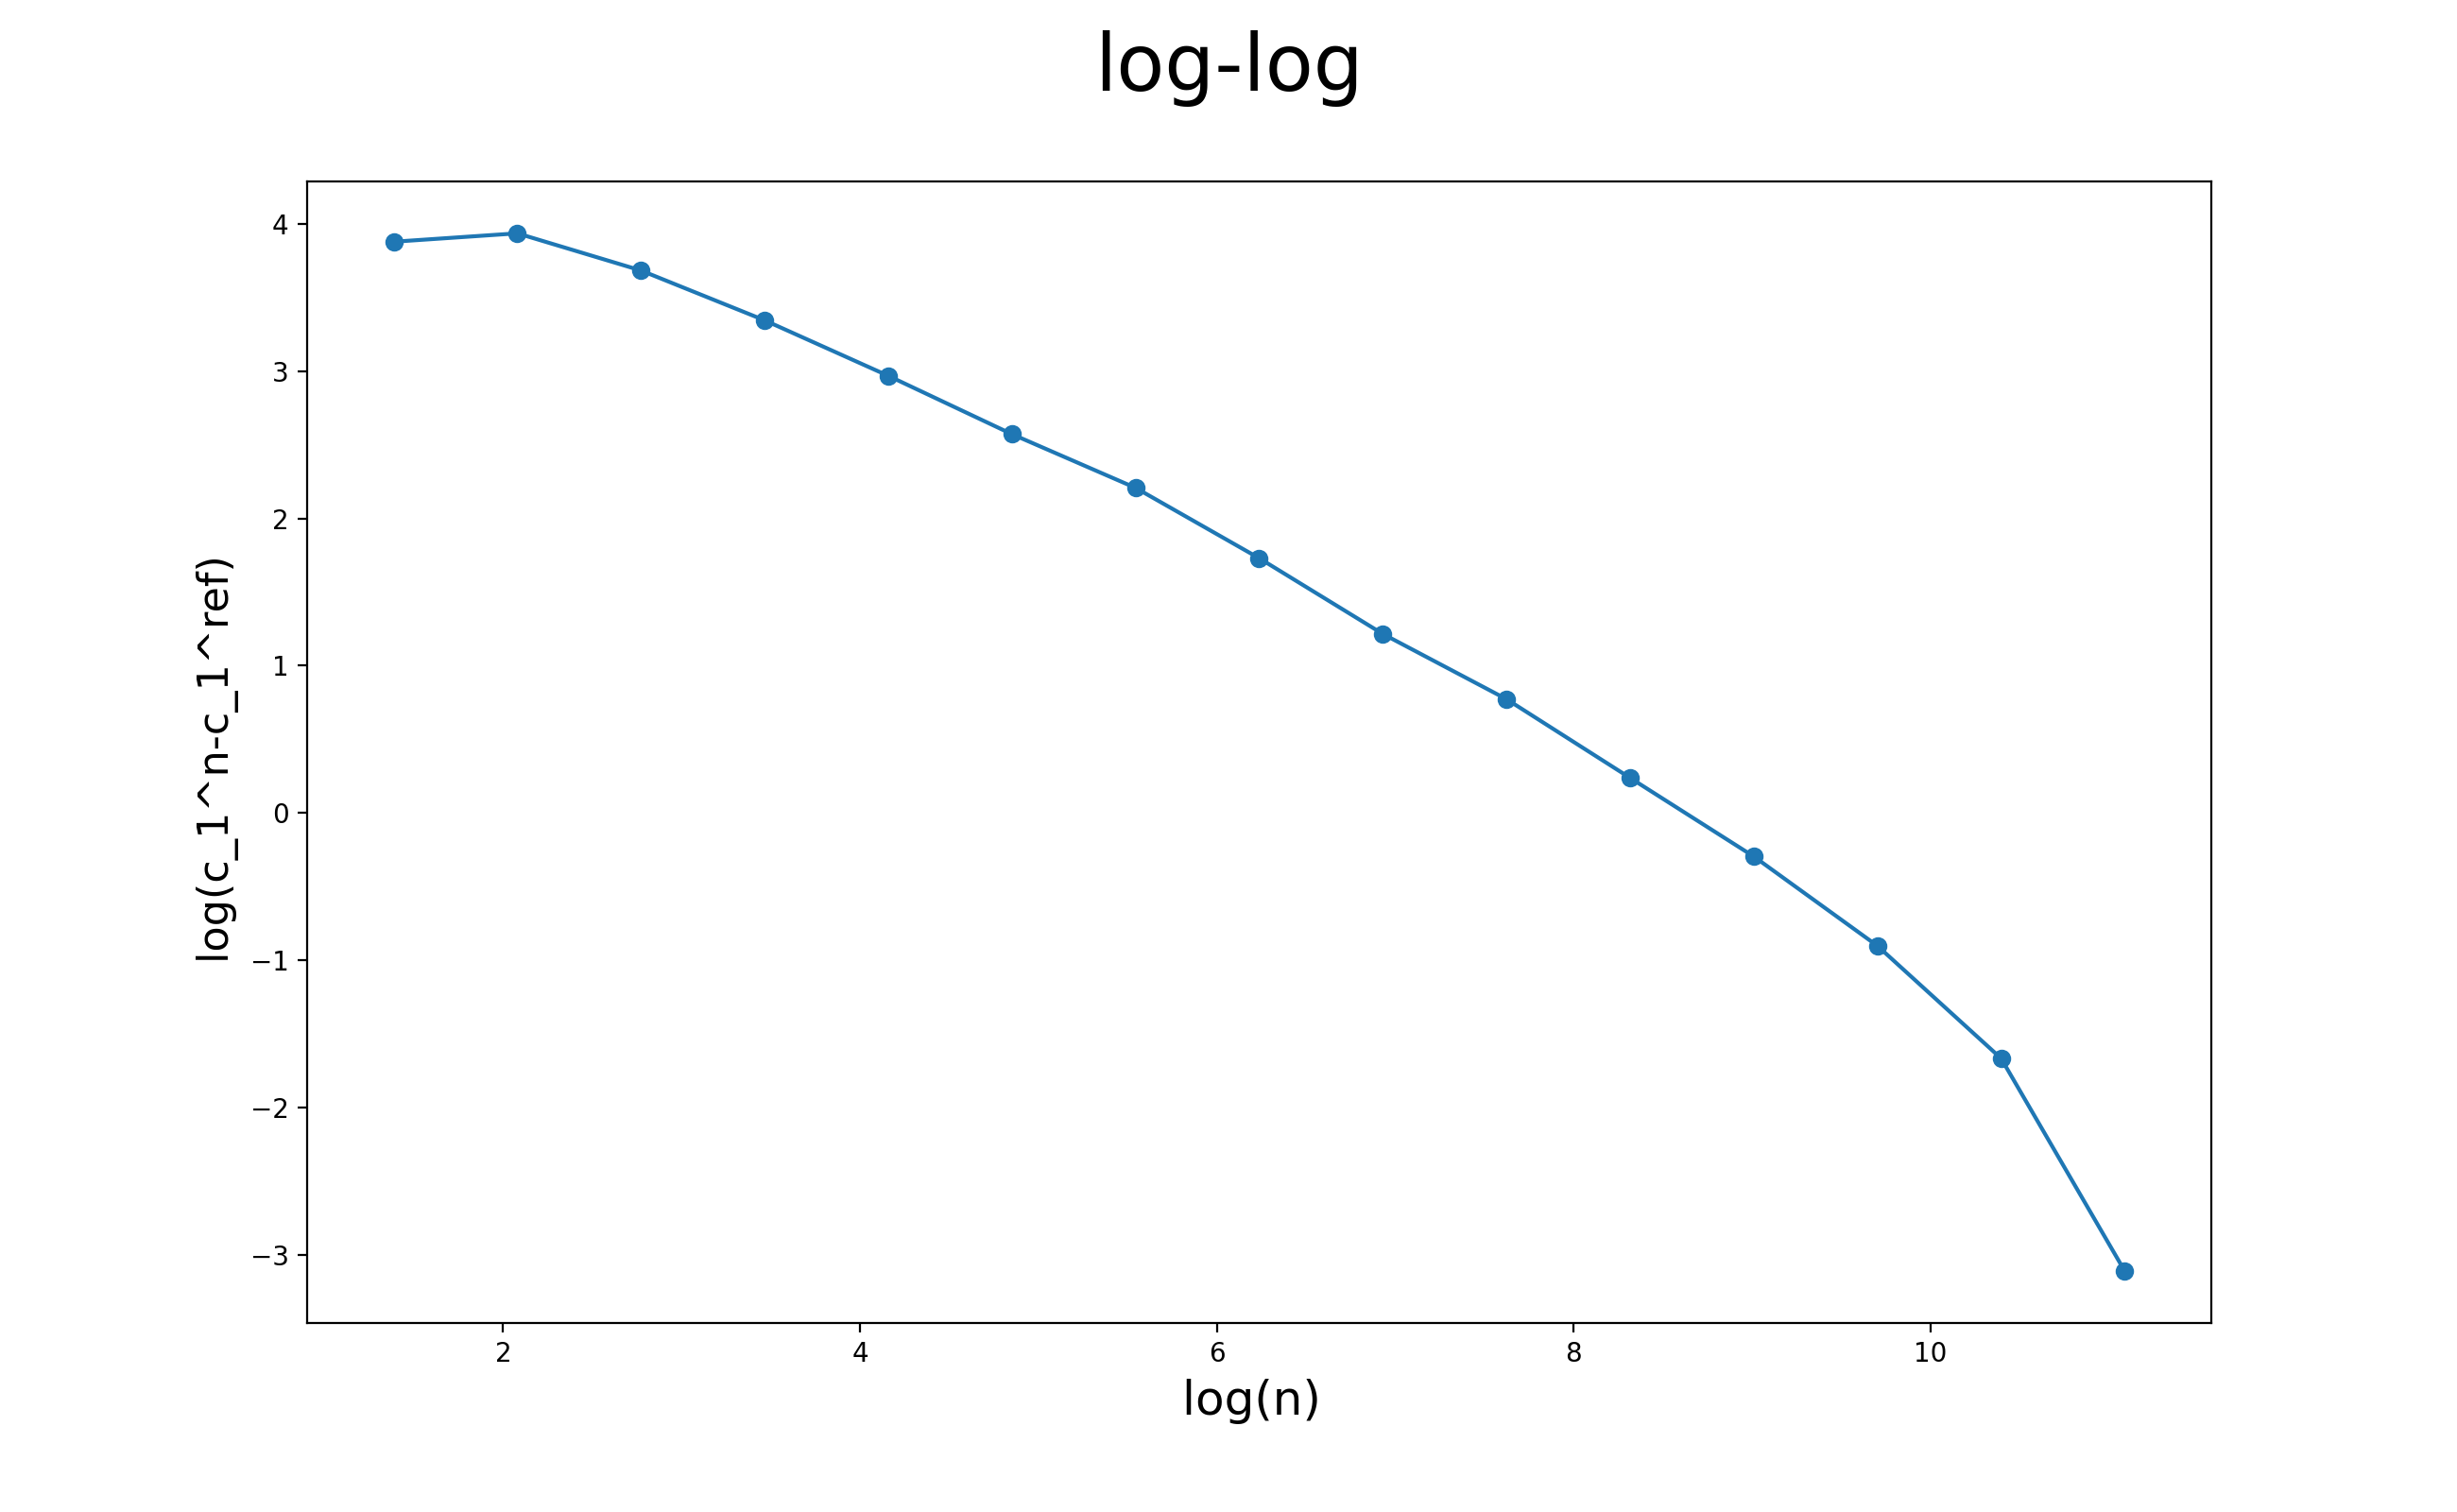
\includegraphics[width=\textwidth, height=55mm]{c1n/c_1log.png}
  \caption{$\log(\bar{c_1}^n-\bar{c_1}^{ref})$ vs $\log(n)$. }\label{c1plotlog}
\end{figure}

\noindent
In this particular case, after applying a linear regression, we obtained that a linear coefficient of $-0.68382593$ is fitting the curve. 
Nevertheless, if the second order RR estimate were true:

$$ \bar{\psi}^n(T) - \psi(T) = \frac{c_1}{n}+\frac{c_2}{n^2} + o(n^{-2}),$$
\noindent
we would have that (considering $c_1 \approx c_1^{ref}$)

\begin{equation}
    \label{eq: compWitBetaLog} 
    \begin{aligned}
    \bar{c_1}^n -c_1^{ref} &= 2n\left(  \bar{\psi}^n(T) - \bar{\psi}^{2n}(T)\right) - c_1^{ref}\\
    &=  2n \left( \frac{c_1}{n} + \frac{c_2}{n^2} - \frac{c_1}{2n} -\frac{c_2}{4n^2} + o(n^{-2}) \right) -c_1^{ref} \\
    &= 2n\left(\frac{c_1}{2n} +\frac{3c_2}{4n^2} + o(n^{-2})\right) -c_1^{ref}
    \\
    & = c_1 +\frac{3c_2}{2n} +o(n^{-1}) -c_1^{ref} \\
    & \approx \frac{3c_2}{2n},
    \end{aligned}
\end{equation}
\noindent
and therefore (where by $\approx$ we mean ``approximately equal" from a non-rigorous mathematical point of view)

\begin{equation}
    \log(\bar{c_1}^n- c_1^{ref}) \approx \log(\frac{3c_2}{n}) = C - \log(n).
\end{equation}
Letting $\log(n) = x$ and $ \log(\bar{c_1}^n- c_1^{ref}) = y$, we have $y=-x+C$. Thus the plot above in Figure \ref{c1plotlog} should be approximately linear with coefficient $-1$, while we obtained $\approx -0.68$.
This tells us that the second order RR estimate might not be true, suggesting an alternative of the form 
\begin{equation}
    \label{eq: estimateRRwithbeta}
    \bar{\psi}^n(T) - \bar{\psi}(T) = \frac{c_1}{n} + \frac{c_2}{n^{2-\beta}} + o(n^{\beta-2}),
\end{equation}
where $\beta \in (0,1)$ might depend on $\lambda, \mu, \nu$. 
Performing similar computations as in \eqref{eq: compWitBetaLog}, yields to 
\begin{equation}
     \log(\bar{c_1}^n- c_1^{ref}) \approx C - (1-\beta) \log(n).
\end{equation}
\noindent
In our particular case it would be $(1-\beta) = -0.6838$, namely $\beta \approx -0.32$. 
\\
However, in all of this, it is noted in \cite{Main} (in Section $4.5$) that the regression coefficient changes as we consider wider ranges of values for $n$ (we are not able to verify this due to limited computation power: for $n=2^{17}$, the evaluation of $\bar{c}_1^n$ already takes four hours).
\\

These observations suggest that the RR estimate of second order (eq. \eqref{eq: moreAccurateEstimate}) and the estimate in equation \eqref{eq: estimateRRwithbeta} do not hold.
 However, all this does not imply that the double step RR extrapolation (described in Subsection \ref{subsection: multiStepRR} and equation \eqref{eq: multiStepRR}) is without any purpose: we remind that $\left\{ \bar{\psi}^n_{_{RR,3}} \right\}_{n \in \mathbb{N}}$ does converge to $\psi$ (as $n\to +\infty$), but the convergence rate \eqref{eq: rr3 convergence rate} might not hold since the second order RR estimate \eqref{eq: moreAccurateEstimate}, from which it follows, seems not to hold. 
\\
Below in Section \ref{section: confirmingRR3} we will compare the computation times between the single step RR extrapolation method and the double step (i.e., computation times in seconds of $\left\{ \bar{\psi}^n_{_{RR,2}} \right\}_{n \in \mathbb{N}}$ and $\left\{ \bar{\psi}^n_{_{RR,3}} \right\}_{n \in \mathbb{N}}$, respectively, for some values of $n$) and the convergence rate in function of $n$.



\subsection{Computational times for the sequence $\left\{ \bar{c}_1^n \right\}_{n\in\mathbb{N}}$.}

From Table \ref{c1table} we can observe that the computation time of $\left\{ \bar{c}_1^n \right\}_{n\in\mathbb{N}}$ increases exponentially with respect to $n$: if $n$ doubles, the computational time (in seconds) of evaluation of $\bar{c}_1^n$ quadruples.
\\
In Figure \ref{comptimes} is presented the plot of $\log$(computation time of $\bar{c}_1^n$) vs $\log(n)$.

Applying a linear regression to the curve in Figure \ref{comptimes}, yields a linear coefficient of $1.99993845$ that is fitting the curve. We could have already expected it by looking at the results in Table \ref{c1table} (for $n=2^{15}$, computing $\bar{c_1}^n$ requires about fifteen minutes, while for  $n=2^{16}$ it takes an hour and for $n=2^{17}$ it takes four hours of computation).

\begin{figure}[ht]
  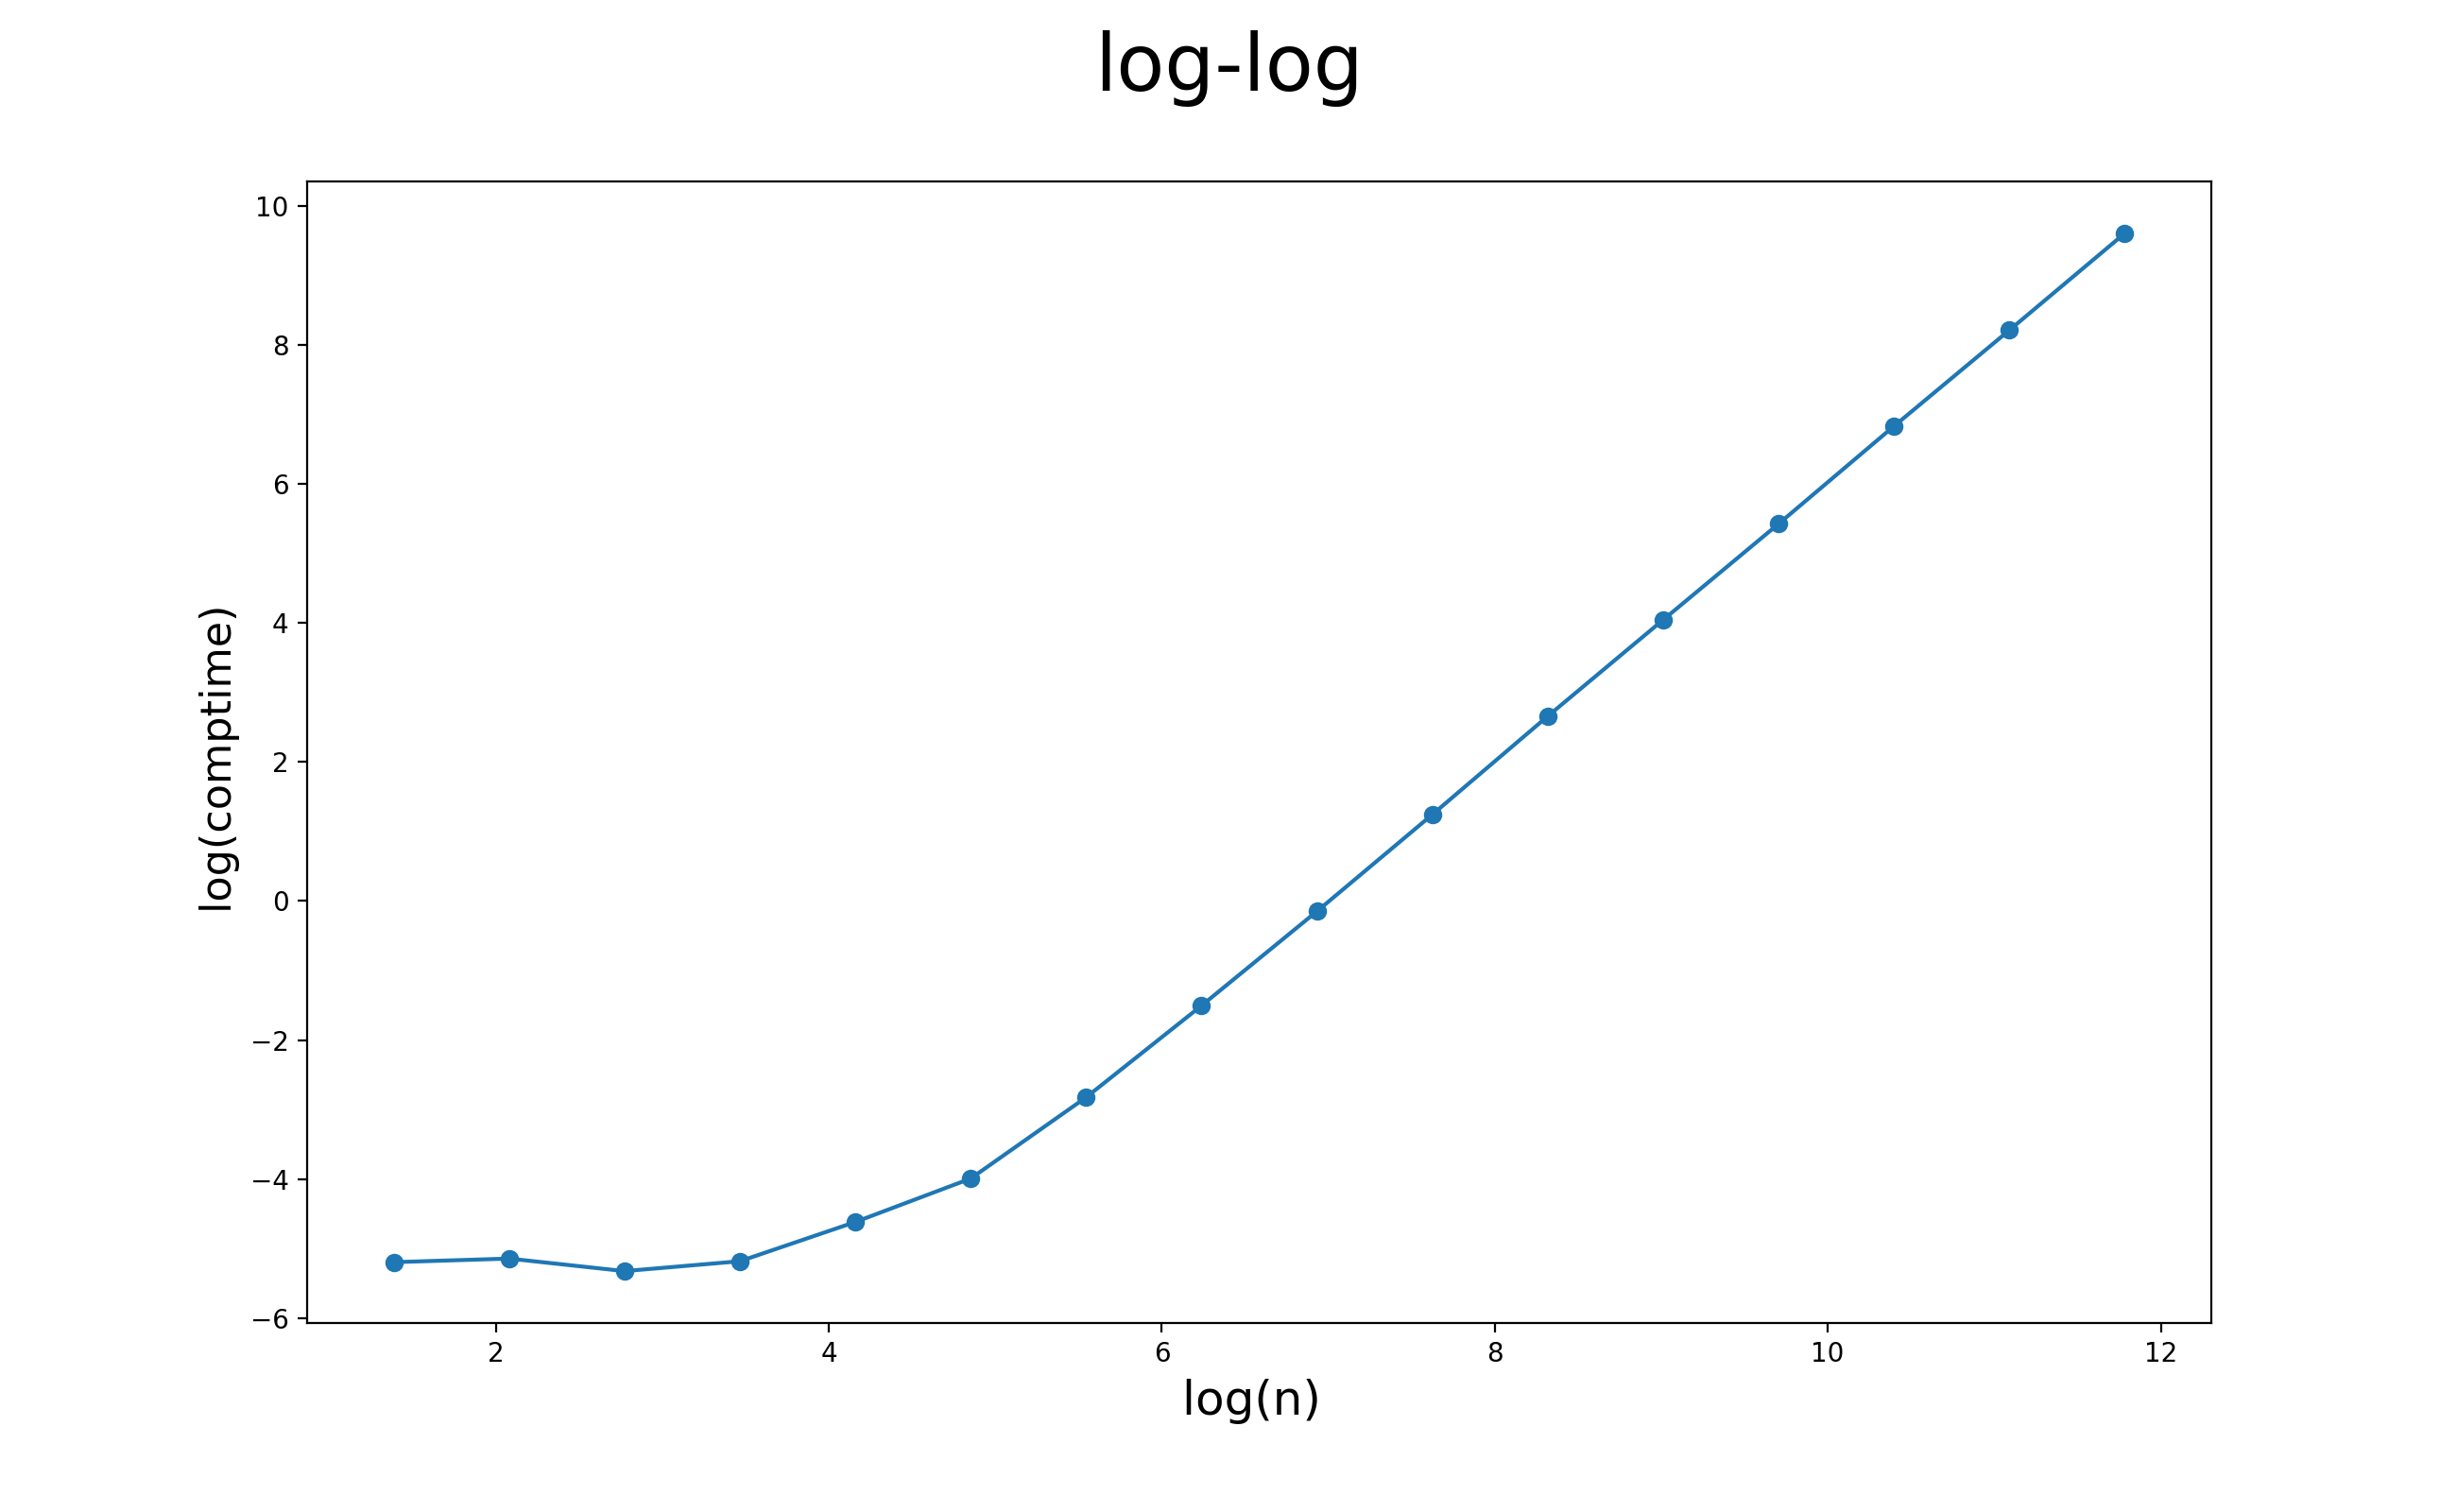
\includegraphics[width=\textwidth, height=55mm]{c1n/comp_times.png}
  \caption{$\log$(computation time of $\bar{c}_1^n$) vs $\log(n)$.}\label{comptimes}
\end{figure}


\newpage

\section{Richardson-Romberg's extrapolations.}
\label{section: confirmingRR3}
Now we compare the single step RR extrapolation (from which we obtain the sequence 
$\left\{ \bar{\psi}^n_{_{RR,2}} \right\}_{n \in \mathbb{N}}$
) with the double step RR extrapolation (from which we obtain the sequence 
$\left\{ \bar{\psi}^n_{_{RR,3}} \right\}_{n \in \mathbb{N}}$
) in terms of computation times\footnote{In seconds. We remind that we use a computer with the following properties: 12 CPUs i7-8750H  @ 2.20GHz. 
Even though the absolute times might change in different machines, we are more interested in ratios among different computation times.} and convergence rate (as $n\to +\infty$). 
\\

We can observe from Table \ref{tavolarichardsonrombergtest1} and Figure \ref{comparisonComExtr} the values of $\bar{\psi}^n_{_{RR,2}}(T)$ and $\bar{\psi}^n_{_{RR,3}}(T)$ for some $n$. The value of $\bar{\psi}^n_{_{RR,3}}(T)$ is computed through equation \eqref{eq: RR.1}, which we recall being
$$\bar{\psi}^n_{_{RR,2}}(T) := 2 \bar{\psi}^n(T) - \bar{\psi}^{\frac{n}{2}}(T).$$
\noindent
While the value of $\bar{\psi}^n_{_{RR,3}}(T)$ is computed through equation \eqref{eq: multiStepRR}, which we recall being
$$\bar{\psi}^n_{_{RR,3}}(T) := \frac{1}{2} \bar{\psi}^{n/4}(T) - 2 \bar{\psi}^{n/2}(T) + \frac{8}{3}\bar{\psi}^n(T).$$

We notice from equations \eqref{eq: multiStepRR} and \eqref{eq: RR.1} that in order to compute $\bar{\psi}^n_{_{RR,2}}(T)$ we need to apply the hybrid Euler scheme through which we evaluate first $\bar{\psi}^n(T)$ and $ \bar{\psi}^{\frac{n}{2}}(T)$.
 Meanwhile, in order to compute $\bar{\psi}^n_{_{RR,3}}(T)$, we need to evaluate $\bar{\psi}^n(T)$, $ \bar{\psi}^{\frac{n}{2}}(T)$ and $ \bar{\psi}^{\frac{n}{4}}(T)$ through the hybrid Euler scheme. 
 Therefore, in terms of computation time, it is expected that the evaluation of $\bar{\psi}^n_{_{RR,3}}(T)$ will require more time than the evaluation of $\bar{\psi}^n_{_{RR,2}}(T)$. 
This is indeed confirmed by the results in Table \ref{tavolarichardsonrombergtest1}, where we can observe that the computation time of $ \bar{\psi}^n_{_{RR,3}}(T)$ in seconds (column ``comp. time RR3") is typically higher than the evaluation of $\bar{\psi}^n_{_{RR,3}}(T)$ (column ``comp. time RR2").
\\

So far, the sequence $\left\{ \bar{\psi}^n_{_{RR,3}}(T)\right\}_{n\in \mathbb{N}}$ seems not to have any advantage over $\left\{ \bar{\psi}^n_{_{RR,2}}(T)\right\}_{n\in \mathbb{N}}$, as it takes more time to be computed. 
However, there is a particular aspect of the double step RR extrapolation: it converges faster as $n\to +\infty$. We can observe this in Figure \ref{comparisonComExtr} where are plotted the curves of $\bar{\psi}^n_{_{RR,3}}(T)$ and $\bar{\psi}^n_{_{RR,2}}(T)$ as functions of $\log(n)$. 
Both curves converge to the same value, as we already know from Remark \ref{remark: rr2 and rr3 do converge}, but $\bar{\psi}^n_{_{RR,3}}(T)$ converges at a faster rate than $\bar{\psi}^n_{_{RR,2}}(T)$, as $n\to +\infty$.
\\

Finally, deciding whether to use $\left\{ \bar{\psi}^n_{_{RR,3}}(T)\right\}_{n\in \mathbb{N}}$ or $\left\{ \bar{\psi}^n_{_{RR,2}}(T)\right\}_{n\in \mathbb{N}}$ in order to approximate the solution $\psi(T)$ to the Riccati differential equation $\mathcal{E}^0_{\lambda, \mu, \nu}$ (equation \eqref{eq: fractionalRiccati}) is up to convenience: if we do not mind about the computation time and want a high accuracy, we can use the double step RR extrapolation. 
Otherwise, if we have limited time and computational power, we can go for the single step RR extrapolation, in exchange of less accuracy. 
Therefore, both the single and double step RR extrapolation might prove useful in different situations.


\begin{table}[ht]
\centering
\begin{tabular}{ |c|c|c|c|c| } 
 \hline
 $n$ & $\bar{\psi}^n_{_{RR,2}}(T)$ & $\bar{\psi}^n_{_{RR,3}}(T)$ & {\small comp. time RR2 (s)} & {\small comp. time RR3  (s)} \\
 \hline
 32 & 766.229560 & 766.466877 & 0.005526 & 0.010074 \\ 
 \hline
 64 & 766.585516 & 766.704169 & 0.006187 & 0.007589 \\ 
 \hline
 128 & 766.724406 & 766.770702 & 0.009566 & 0.010336 \\ 
 \hline
 256 & 766.774044 & 766.790590 & 0.019738 & 0.019968 \\
 \hline
 512 & 766.789657 & 766.794862 & 0.061665 & 0.065757 \\
 \hline
 1024 & 766.796395 & 766.798641 & 0.227041 & 0.241486 \\
 \hline
 2048 & 766.798607 & 766.799345 & 0.913140 & 0.979847 \\
 \hline
 4096 & 766.799196 & 766.799392 & 3.645494 & 4.026486 \\
 \hline
 8192 & 766.799415 & 766.799488 & 14.967328 & 15.561022 \\
 \hline
 16384 & 766.799479 & 766.799501 & 60.779404 & 62.147462 \\
 \hline
 32768 & 766.799500 & 766.799507 & 248.358794 & 308.513195 \\
 \hline
\end{tabular}
\caption{Richardson Romberg's estimates and computation times.}
\label{tavolarichardsonrombergtest1}
\end{table}


\begin{figure}[ht]
  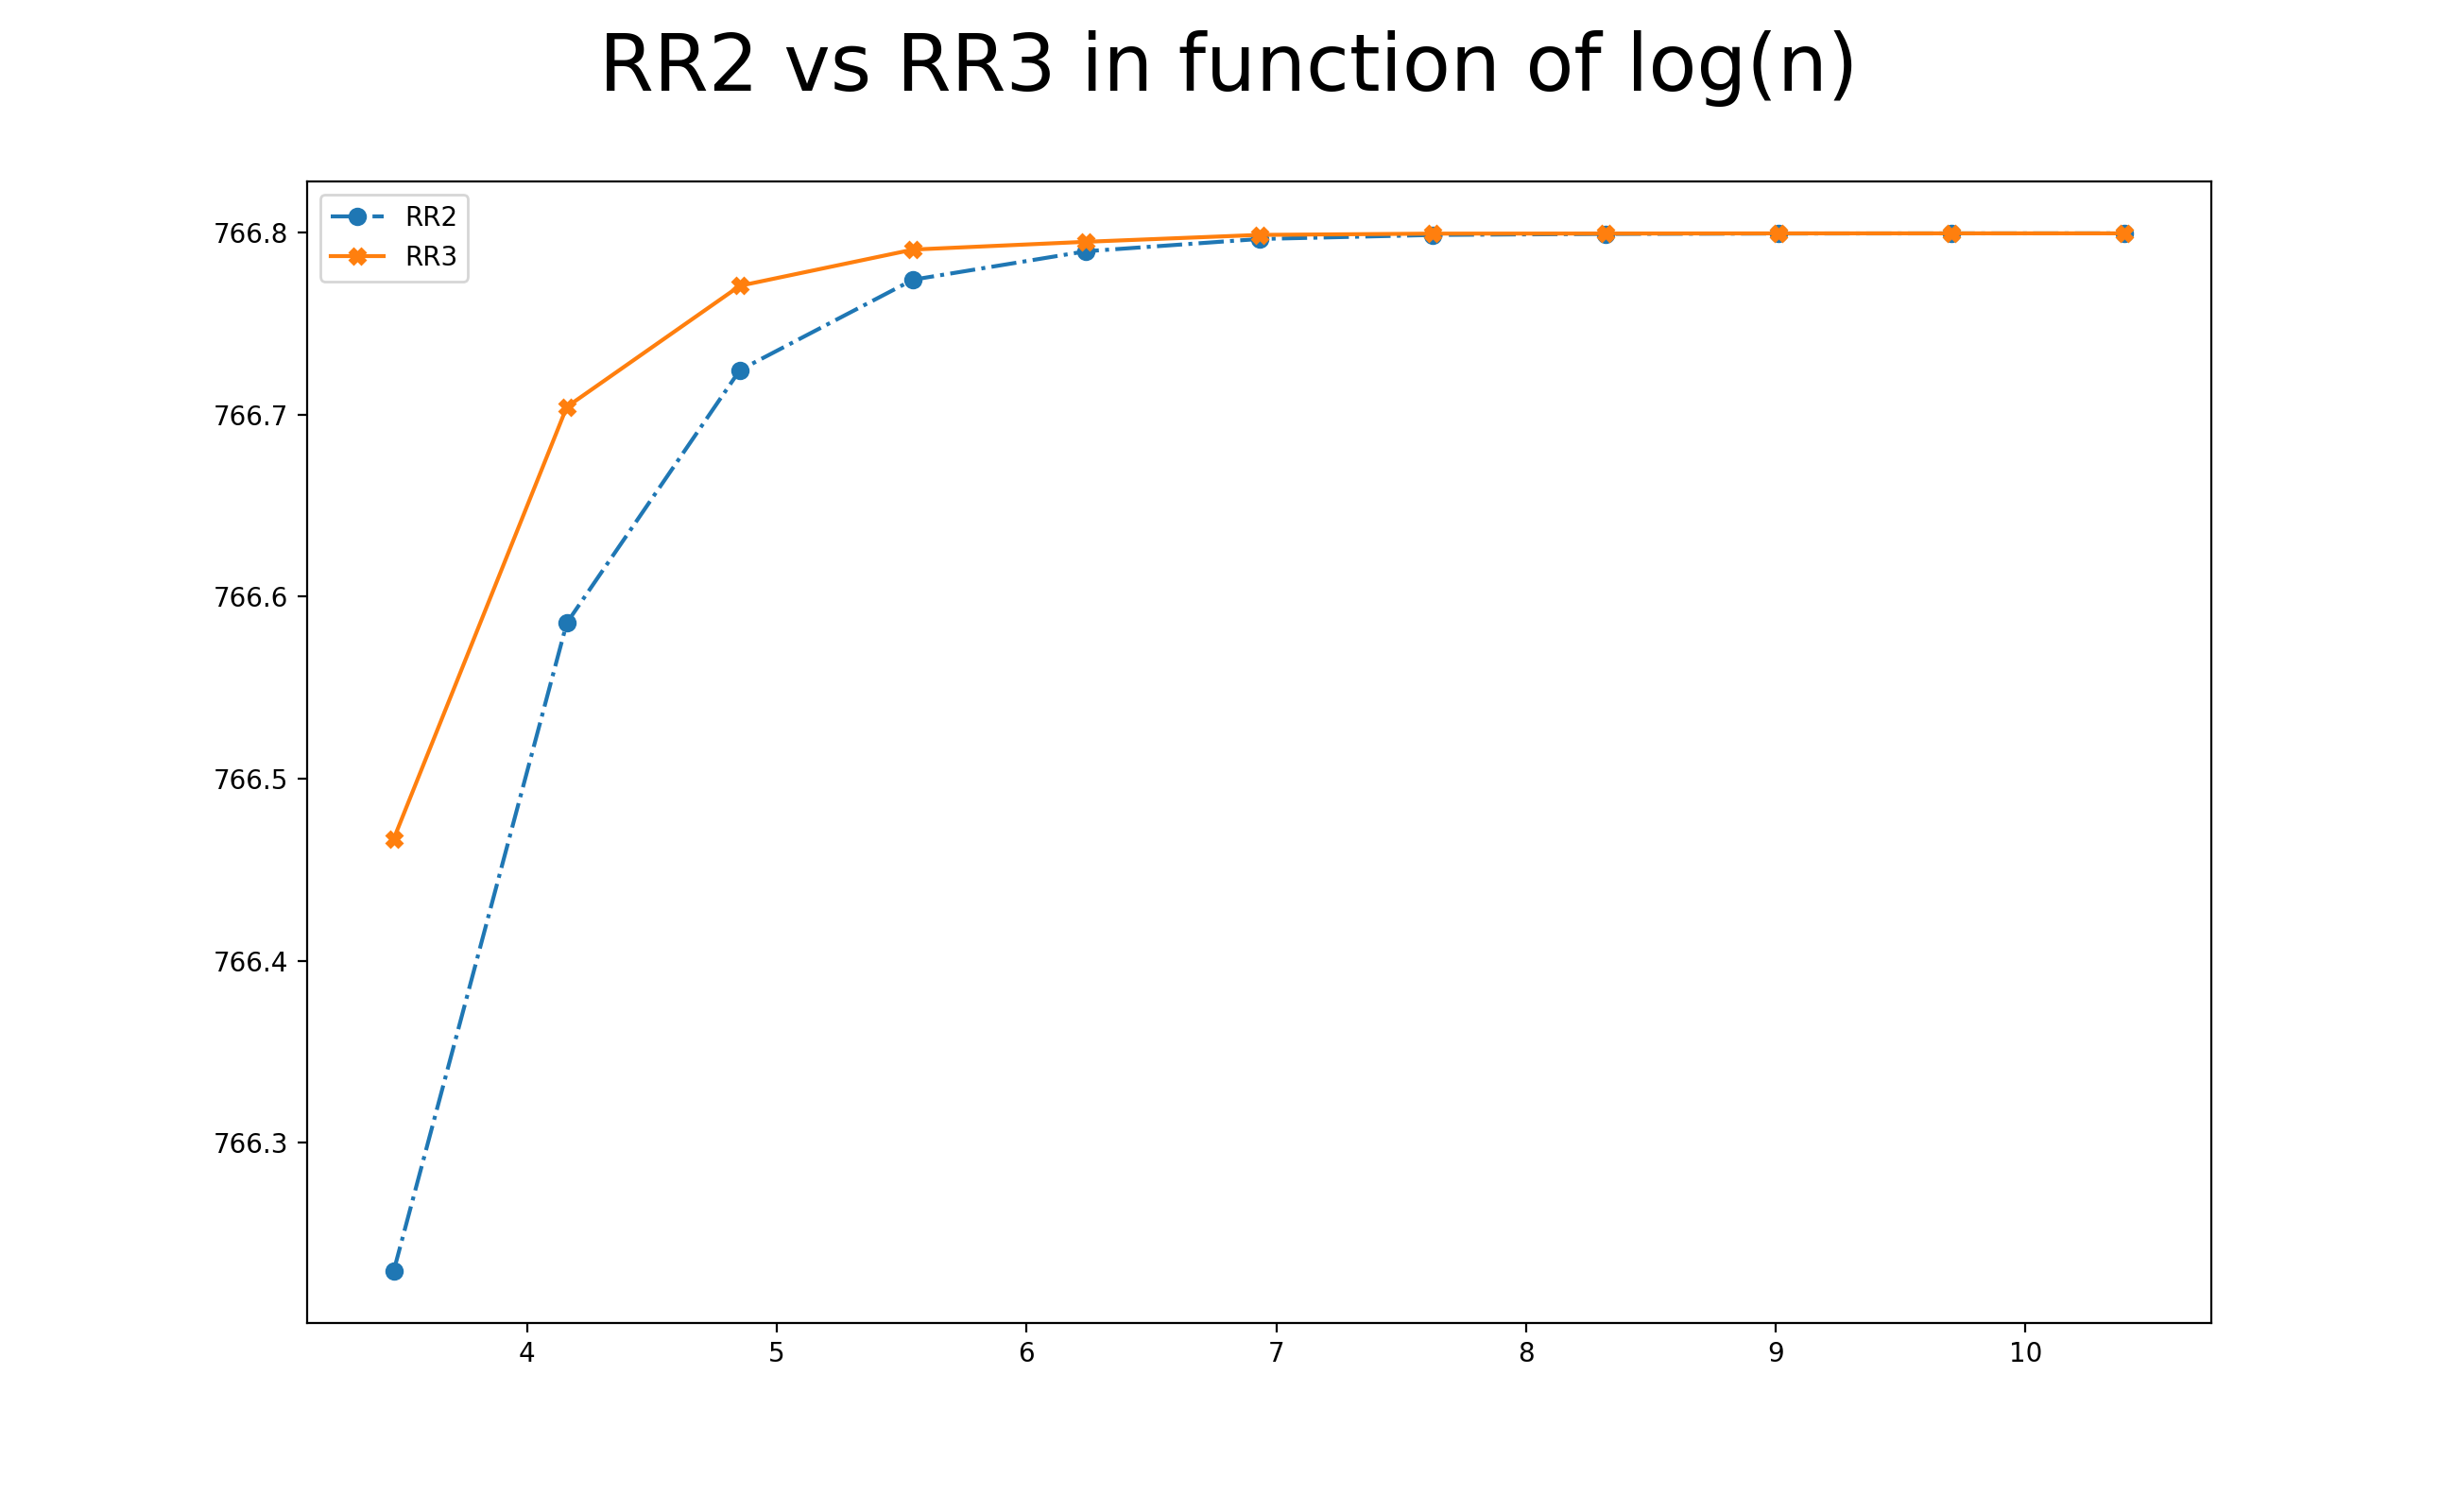
\includegraphics[width=\textwidth, height=55mm]{extrapolated/extrapolated.png}
  \caption{$RR2$ vs $RR3$: the red and blue lines are $\bar{\psi}^n_{RR,3}(T)$ and $\bar{\psi}^n_{RR,2}(T)$, respectively, as functions of $\log(n)$.
 This comes from the test with parameters \eqref{eq: NumericalTestParameters}.}\label{comparisonComExtr}
\end{figure}


\section{Another Test with different parameters.}
In this Section we run again the hybrid Euler scheme with a different set of parameters and will observe whether the previous analyzied behaviours are mantained or not. The parameters used in this test are:
\begin{equation}
    \label{eq: NumericalTestParameters2}
    \alpha = 0.64, \hspace{0.2cm} \lambda = 0.2, \hspace{0.2cm} \mu = - 200 , \hspace{0.2cm} \nu= 200.
\end{equation}
This set of parameters still contains the rough behaviour of the fractional Brownian motion ($\alpha = 0.64 \rightarrow H = \alpha - \frac{1}{2} = 0.14< \frac{1}{2}$).
We also set $T=\frac{1}{252}$, the accuracy $\epsilon_0=0.01$ and $r_{max}=105$ (also in this case we chose $r_{max}=105$ due to machine's limitations\footnote{Computing the $107$-th coefficient was already impossible for the machine, as it exceeded the maximum number representable in the memory.}).
\\

The coefficients of the fractional power series $\psi(t) = \sum_{k=0}^{+\infty} a_kt^{k\alpha}$ that we obtained are partially presented in Table \ref{tavolacoefficientstest2}.


\begin{table}[ht]
\centering
\begin{tabular}{ |c|c| |c|c| |c|c| } 
 \hline
 $k$ & $a_k$ & $k$ & $a_k$ & $k$ & $a_k$\\ 
 \hline
 0 & 0 & 40 & $-1.687936 \cdot 10^{74}$ & 95 & $1.354194 \cdot 10^{174}$\\ 
 \hline
 1 & 2.225580\cdot 10^{2} & 41 & 1.102731 \cdot 10^{76} & 96 & $-8.890316 \cdot 10^{175}$\\ 
 \hline
 2 &  -3.469453\cdot 10^{4} & 42 & -7.205620 \cdot 10^{77} & 97 & $5.836737 \cdot 10^{177}$\\
 \hline
 3 &  4.307108\cdot 10^{6} & 43 &  4.709280\cdot 10^{79} & 98 & $-3.832122 \cdot 10^{179}$\\
 \hline
 4 &  -4.526010\cdot 10^{8} & 44 & -3.078325\cdot 10^{81} & 99 & $2.516080 \cdot 10^{181}$\\
 \hline
 5 &  4.174764\cdot 10^{10} & 45 & 2.012555\cdot 10^{83} & 100 & $-1.652058 \cdot 10^{183}$\\
 \hline
 6 &  -3.465067\cdot 10^{12} & 46 & -1.315989\cdot 10^{85} & 101 & $1.084779 \cdot 10^{185}$\\
 \hline
 7 &  2.637354\cdot 10^{14} & 47 & 8.606478\cdot 10^{86} & 102 & $-7.123154 \cdot 10^{186}$\\
 \hline
 8 &  -1.870412\cdot 10^{16} & 48 & -5.629447\cdot 10^{88} & 103 & $4.677547 \cdot 10^{188}$\\
 \hline
 9 &  1.254454\cdot 10^{18} & 49 & 3.682738\cdot 10^{90}& 104 & $-3.071697 \cdot 10^{190}$\\
 \hline
\end{tabular}
\caption{coefficients $\left\{ a_k \right\}_{k \in \mathbb{N}}$ of the fractional power series $\psi(t) = \sum_{k=0}^\infty a_k t^{k\alpha}$.}
\label{tavolacoefficientstest2}
\end{table}
\noindent
In this case the growth of the absolute values of the coefficients $\left\{ |a_k| \right\}_{k\in \mathbb{N}}$ is also exponential, as we can see in Figure \ref{barbaz2}, where is presented $f(k):=\log(|a_k|)$ for $k=0,1,\cdots, 105$.

%\eqref{eq: NumericalTestParameters2} 
%\eqref{eq: NumericalTestParameters}

\begin{figure}[ht]
  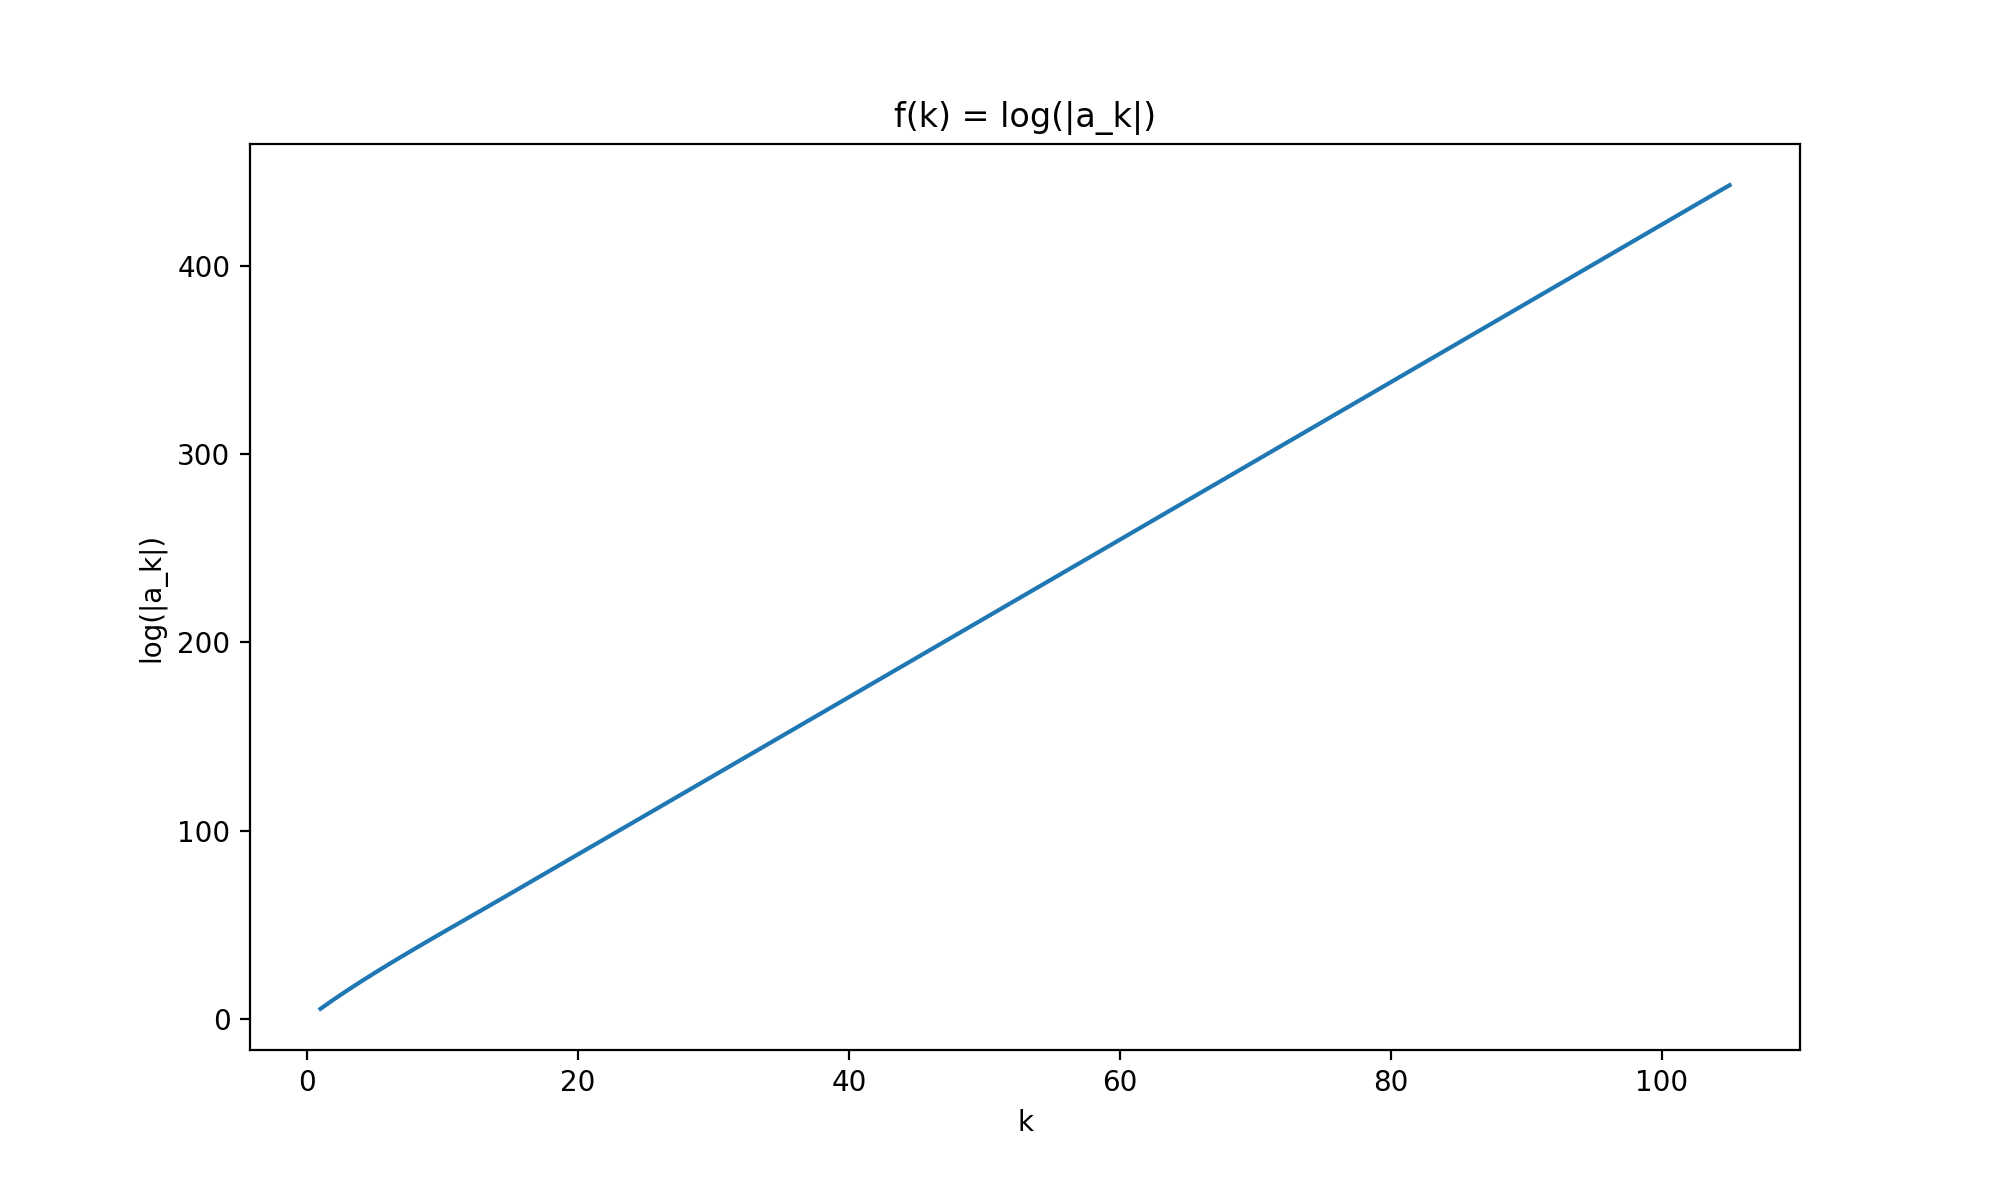
\includegraphics[width=\textwidth, height=50mm]{coefficients_test_2/output.png}
  \caption{plot of the curve $f(k) = \log(|a_k|)$, $k=0,1,\cdots,105$, confirming, also in this test, the exponential growth of the absolute values of the coefficients $\left\{|a_k|\right\}_{k\in\mathbb{N}} $ of $\psi(t) = \sum_{k=0}^\infty a_kt^{k\alpha}$.}\label{barbaz2}
\end{figure}

Using the Euler Discretization scheme we computed some $\bar{\psi}^n$. In Figure \ref{fig: ante2psi_16}, \ref{fig: ante2psi_64} and \ref{fig: ante2psi_256} are displayed, respectively, $\bar{\psi}^n$ for $n= 16, 64, 256$. The shape of the curves is not far from that of the previous test (see Figure \ref{fig: psi n=16}, \ref{fig: psi n=64} and \ref{fig: psi n=256}).


\begin{figure}[pH]
  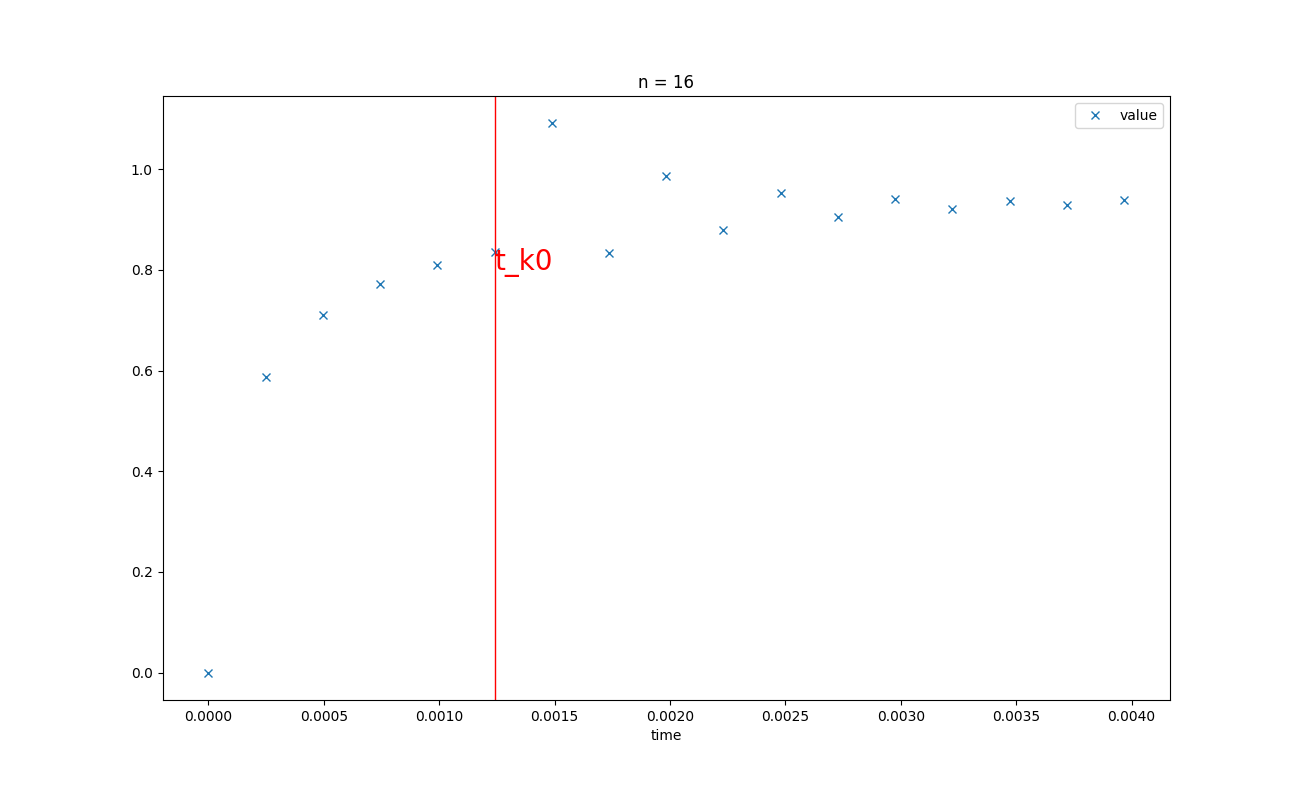
\includegraphics[width=\textwidth, height=60mm]{coefficients_test_2/n = 16.png}
  \caption{(a) curve of $\bar{\psi}^{16}(t)$ evaluated at $t=t_0,t_1,\cdots ,t_{16}$.}\label{fig: ante2psi_16}
\end{figure}

\begin{figure}[pH]
  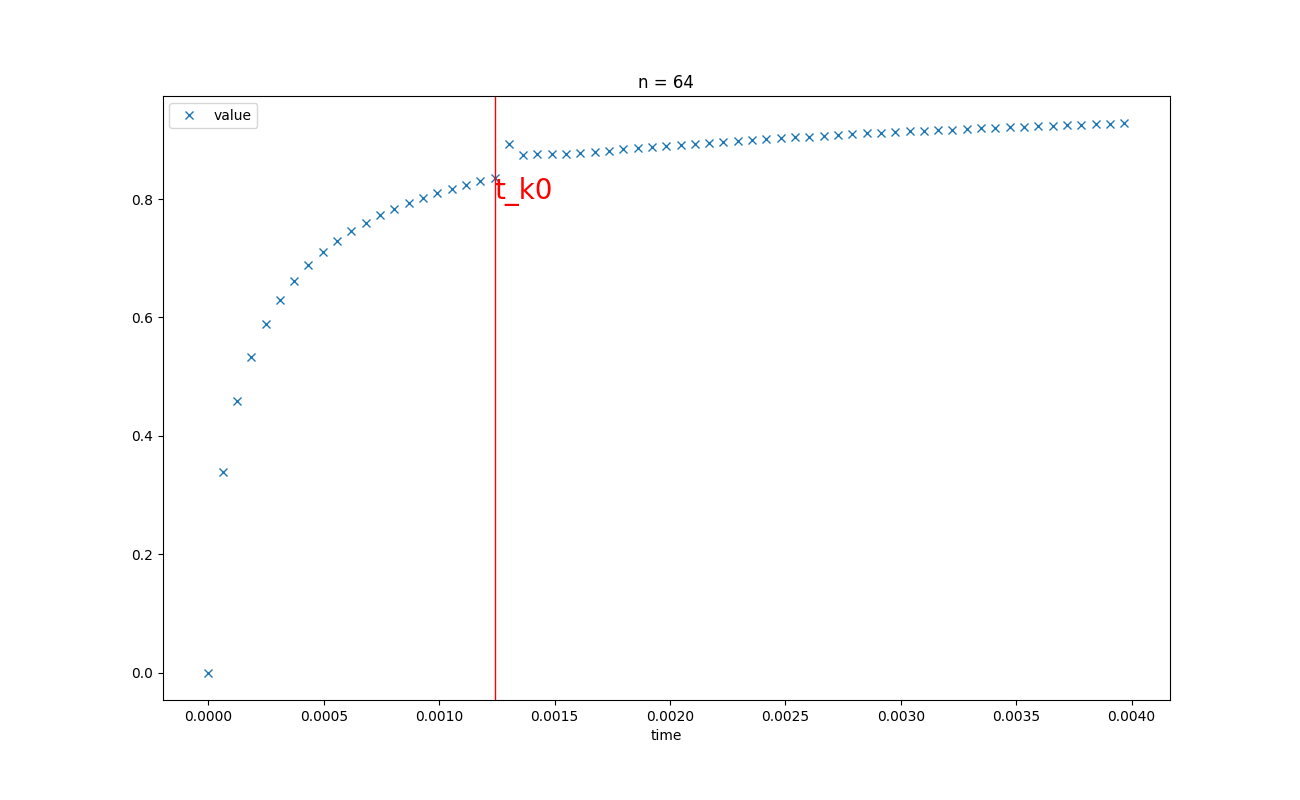
\includegraphics[width=\textwidth, height=60mm]{coefficients_test_2/n = 64.png}
  \caption{(b) curve of $\bar{\psi}^{64}(t)$ evaluated at $t=t_0,t_1,\cdots ,t_{64}$.}\label{fig: ante2psi_64}
\end{figure}

\begin{figure}[pH]
  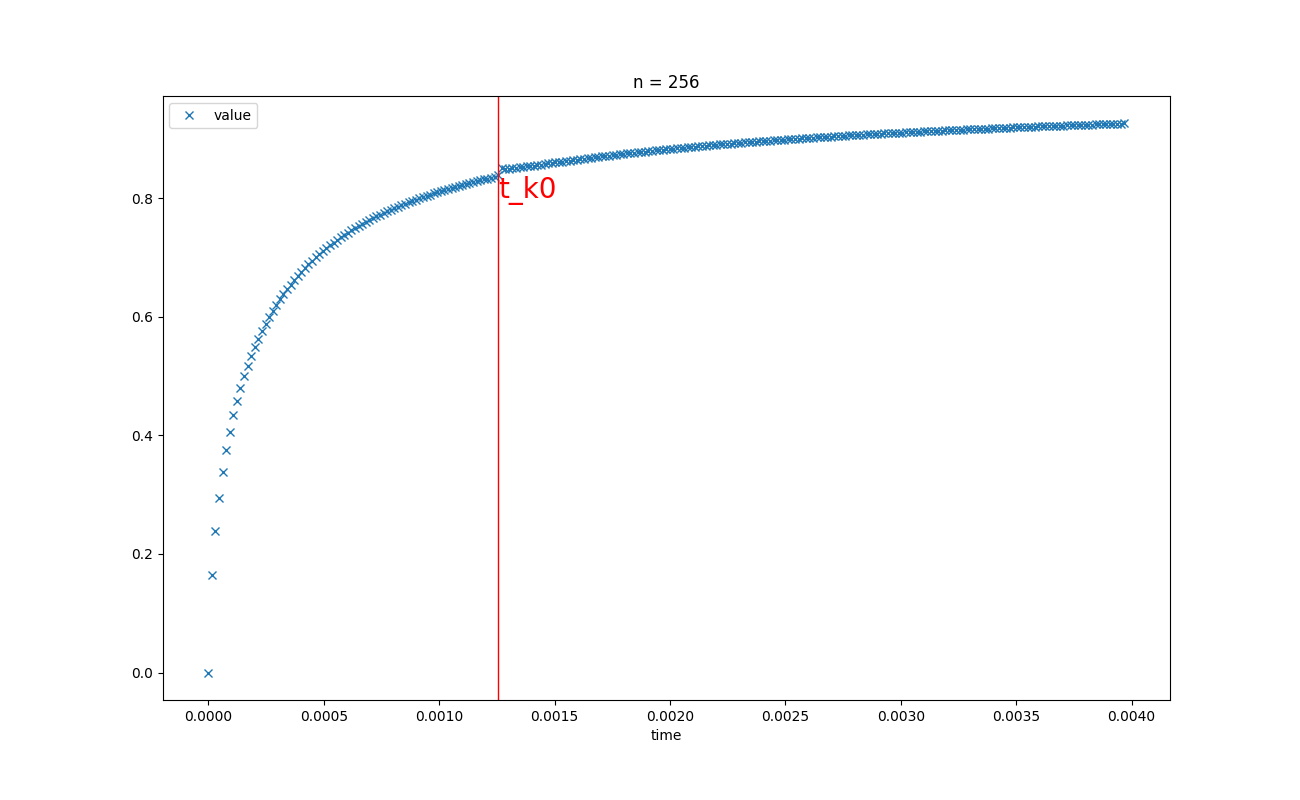
\includegraphics[width=\textwidth, height=60mm]{coefficients_test_2/n = 256.png}
  \caption{(c) curve of $\bar{\psi}^{256}(t)$ evaluated at $t=t_0,t_1,\cdots ,t_{256}$.}\label{fig: ante2psi_256}
\end{figure}

As for the sequence $\left\{\bar{c_1}^n \right\}_{n\in \mathbb{N}}$ (recall eq. \ref{eq: 32inthepaper}), the results are presented in Table \ref{tavolavaluesofc1test2} and Figure \ref{c1plot2}. Notice that also in this case the sequence $\bar{c}_1^n$ converges. Moreover, the ratio of consecutive computation times (last column in Table \ref{tavolavaluesofc1test2}) has a similar behaviour to that from the previous test (Table \ref{c1table}): for $n$ large enough, its value is around four.

\begin{table}[ht]
\centering
\begin{tabular}{ |c|c|c|c| } 
 \hline
 $n$ & $\bar{c_1}^n$ & {\footnotesize computation time (seconds)} & {\footnotesize ratio of consecutive computation times} \\ 
 \hline
4	&45.992298 &	0.000978 &	NaN \\
\hline
8	&-18.911034	& 0.001066	&1.089956 \\
\hline
16	&0.262637	& 0.001241 &	1.164169 \\
\hline
32	&0.161077 &	0.002010 &	1.619789 \\
\hline
64	&0.151405 &	0.004920 &	2.447515 \\
\hline
128	&0.143325 &	0.016612 &	3.376496 \\
\hline
256	&0.140296 &	0.057853 &	3.482662 \\
\hline
512	&0.137850 &	0.225938 &	3.905420 \\
\hline
1024 &	0.135780 &	0.904298 &	4.002411 \\
\hline
2048 &	0.134314 &	3.672320 &	4.060962 \\
\hline
4096 &	0.133632 &	14.989243 &	4.081682 \\
\hline
8192 &	0.132789 &	60.255214 &	4.019897 \\
 \hline
\end{tabular}
\caption{evaluations of $\bar{c_1}^n$ (defined in equation \eqref{eq: 32inthepaper}) and computation times.}
\label{tavolavaluesofc1test2}
\end{table}

\begin{figure}[ht]
  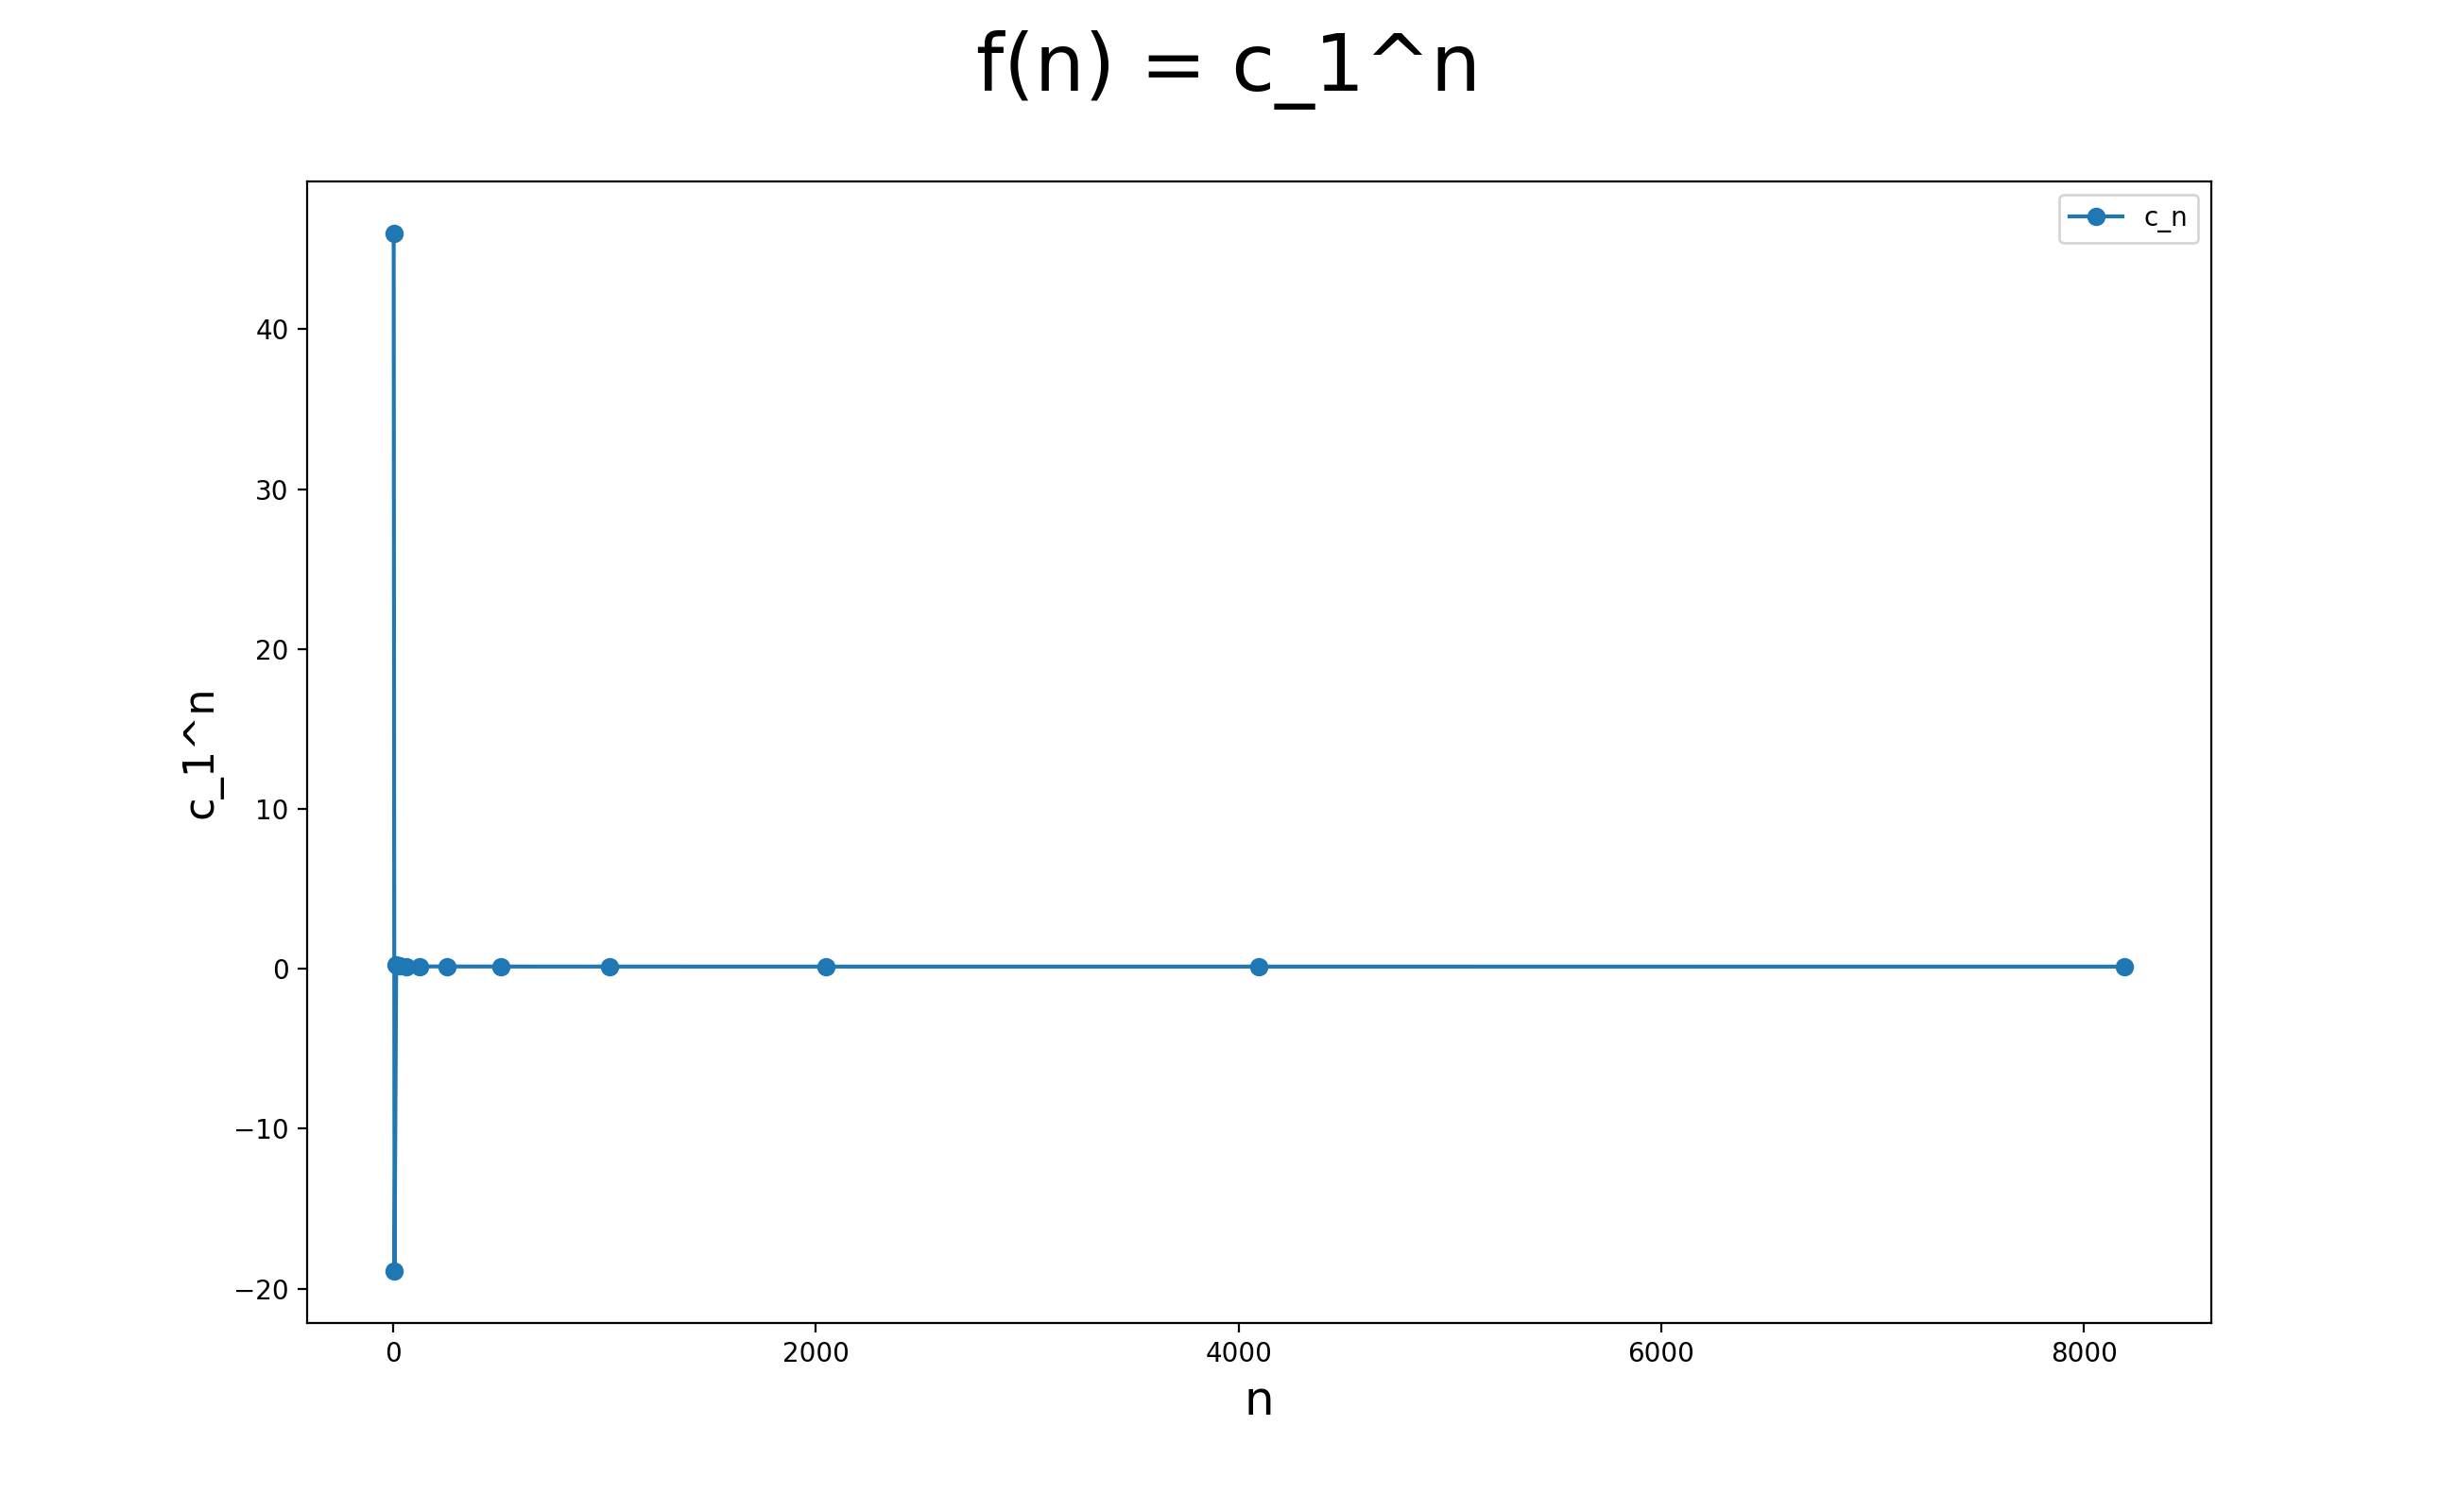
\includegraphics[width=\textwidth, height=60mm]{coefficients_test_2/c_1^n.png}
  \caption{we plot $\bar{c}_1^n$ as a function of $n$: $f(n):=\bar{c}_1^n $.}\label{c1plot2}
\end{figure}

Finally, we applied the Richardson-Romberg extrapolation (single and double step). 
The results are displayed in Table \ref{tavolarichardsonrombergtest2},
 Figure \ref{comparisonComExtr2} and \ref{comparisonComExtr2_fine}, 
 where we notice that the sequences $\left\{ \bar{\psi}^n_{RR,3}(T)\right\}_{n\in\mathbb{N}}$ and $\left\{ \bar{\psi}^n_{RR,2}(T)\right\}_{n\in\mathbb{N}}$ converge to the same value.

\begin{table}[ht]
\centering
\begin{tabular}{ |c|c|c|c|c| } 
 \hline
 $n$ & RR2 & RR3 & {\small comp. time RR2 (s)} & {\small comp. time RR3 (s)} \\
 \hline
32   & 	0.922013	& 0.522561	& 0.002253	& 0.002648   \\
\hline
64  & 	0.925187	& 0.926245	& 0.003159	& 0.003967 \\
\hline
128	  &   0.925338	& 0.925388	& 0.005185	& 0.006413 \\
\hline
256  & 	0.925401	& 0.925422	& 0.016054	& 0.017432 \\
\hline
512	  &   0.925413	& 0.925417	& 0.061595	& 0.062513 \\
\hline
1024  & 	0.925417	& 0.925419	& 0.220778	& 0.232190 \\
\hline
2048  & 	0.925420	& 0.925420	& 0.852463	& 0.906958 \\
\hline
4096& 	0.925420	& 0.925420	& 3.378545	& 3.681777 \\
\hline
8192  & 	0.925420	& 0.925420	& 13.629304	& 14.739946 \\
\hline
16384  & 	0.925421	& 0.925421	& 54.030256	& 58.376655 \\
\hline
32768  & 	0.925421	& 0.925421	& 215.273587	& 226.938969 \\
\hline
\end{tabular}
\caption{Richardson Romberg's estimates and computation times.}
\label{tavolarichardsonrombergtest2}
\end{table}


\begin{figure}[ht]
  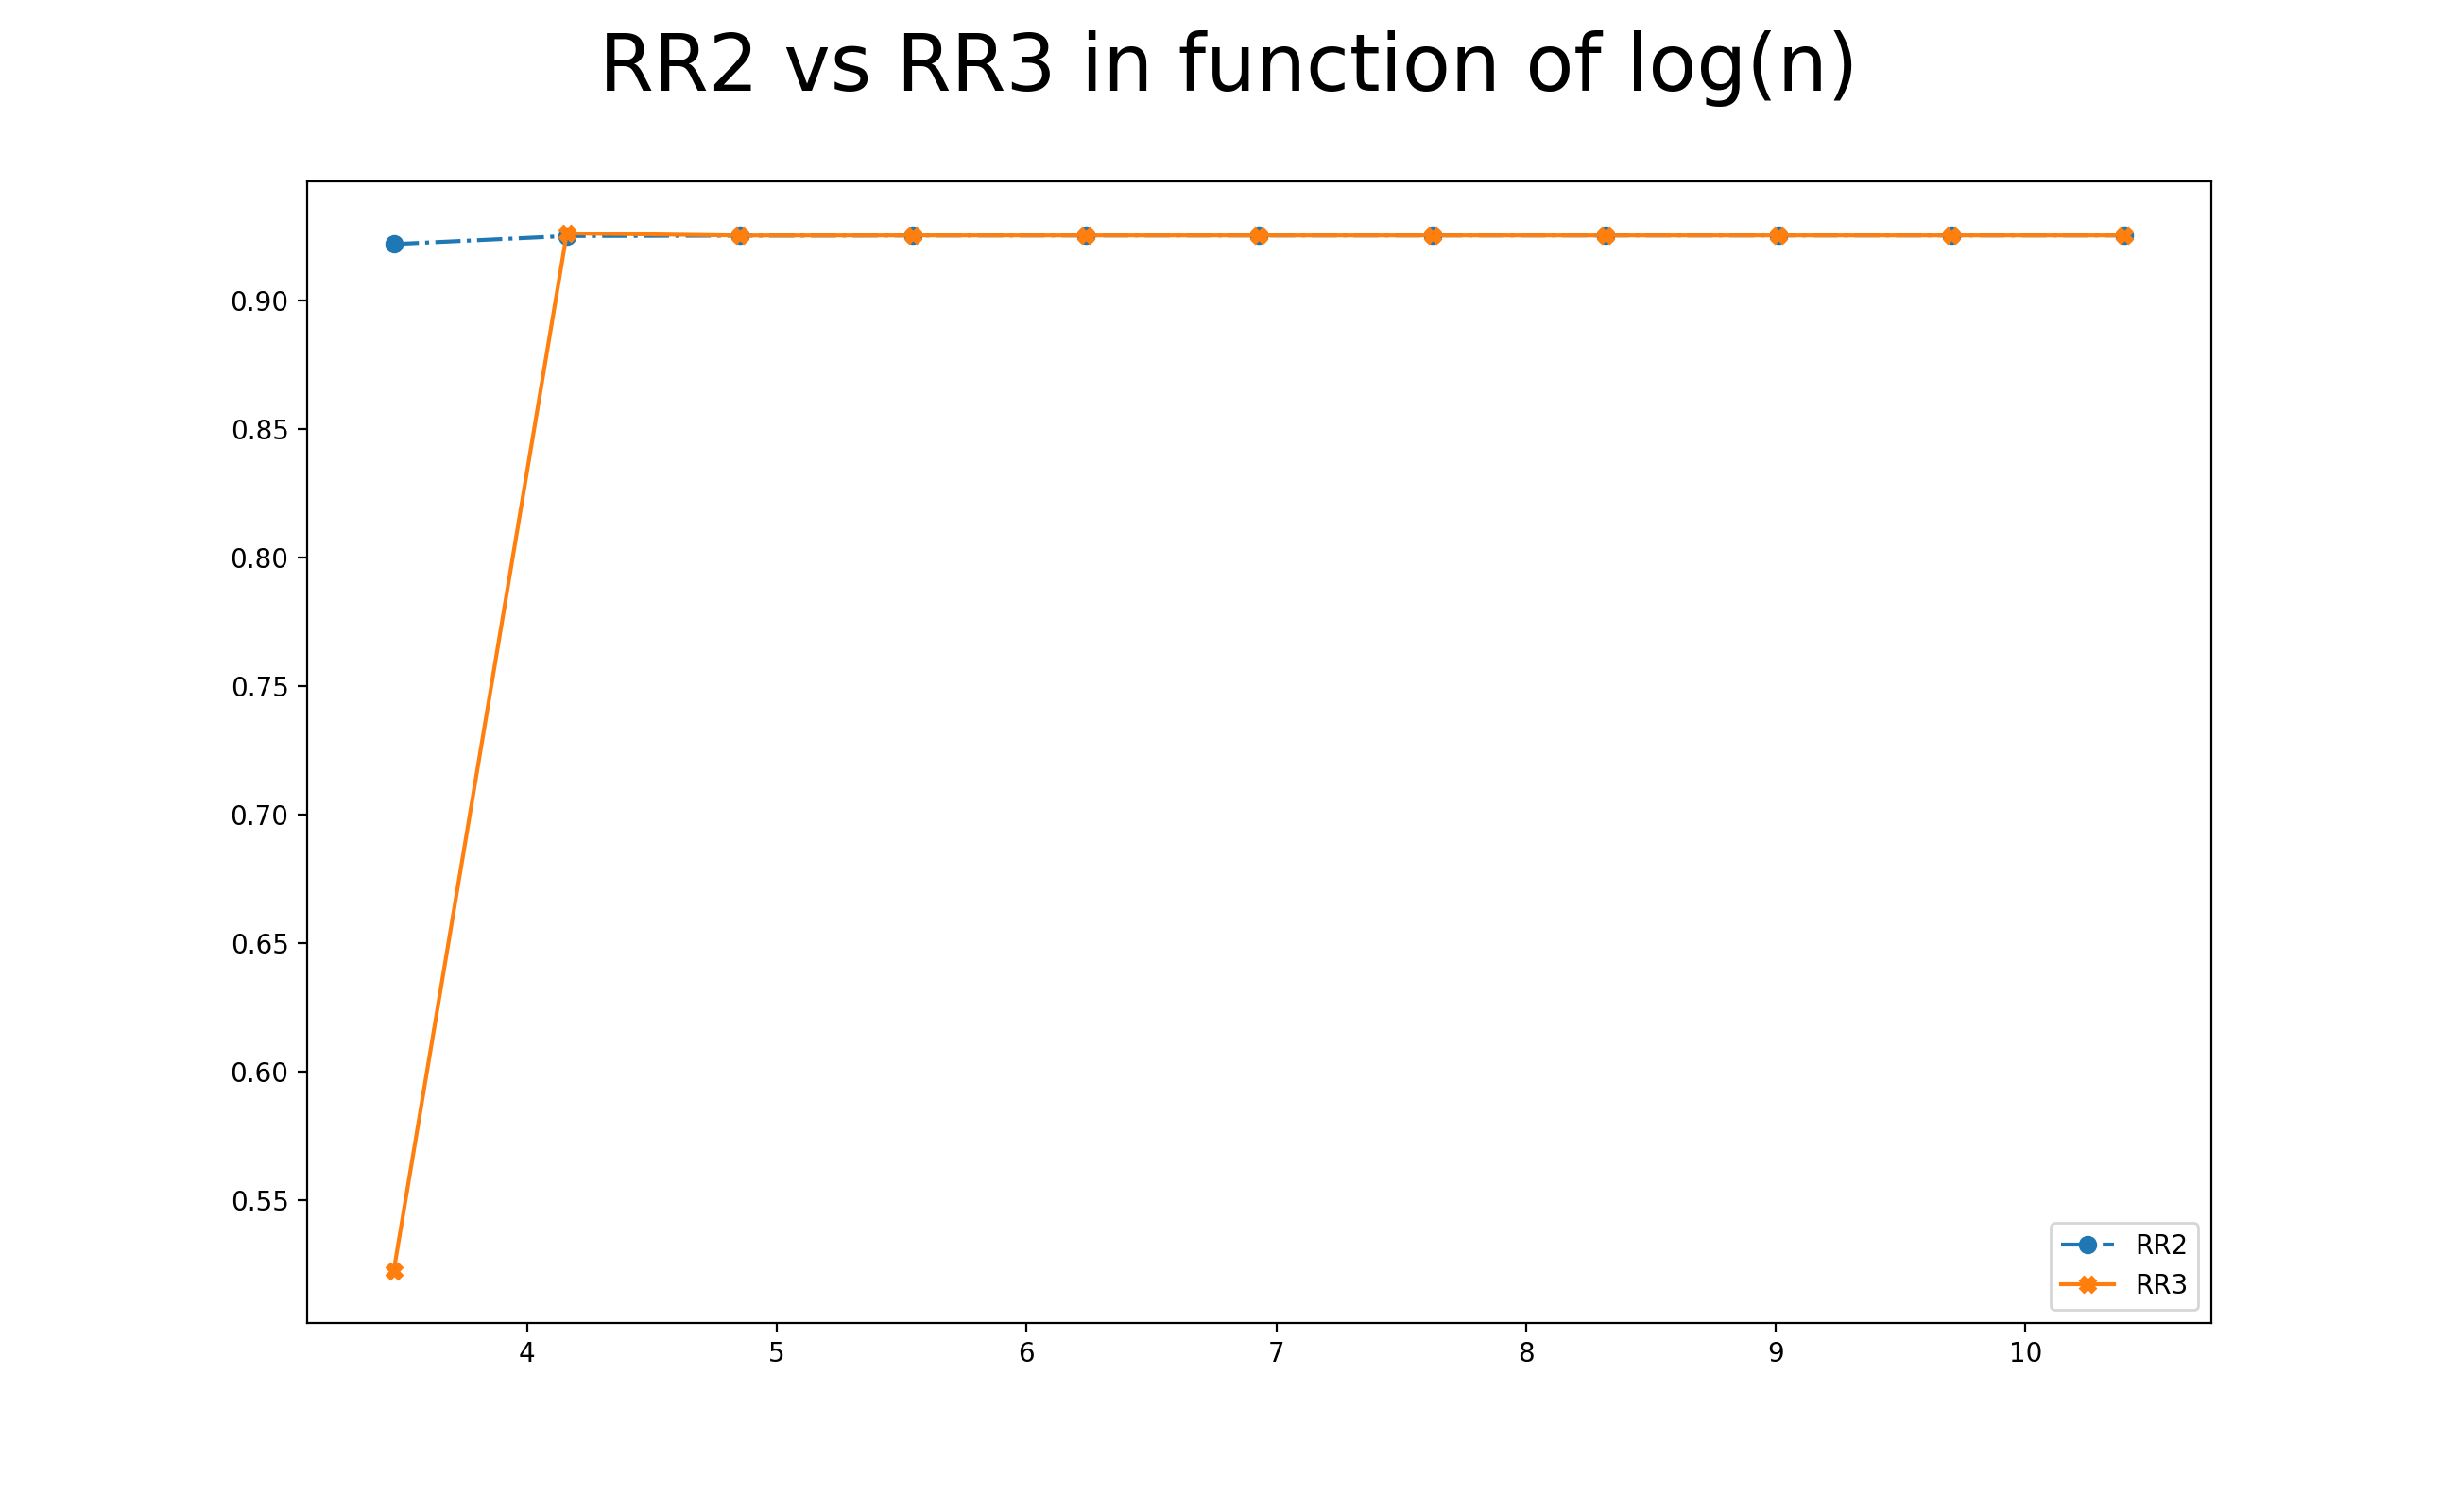
\includegraphics[width=\textwidth, height=60mm]{coefficients_test_2/extrapolatedrr.png}
  \caption{$RR2$ vs $RR3$: the red and blue lines are $\bar{\psi}^n_{RR,3}(T)$ and $\bar{\psi}^n_{RR,2}(T)$, respectively, as functions of $\log(n)$. This comes from the test with parameters \eqref{eq: NumericalTestParameters2}.}\label{comparisonComExtr2}
\end{figure}


\begin{figure}[ht]
  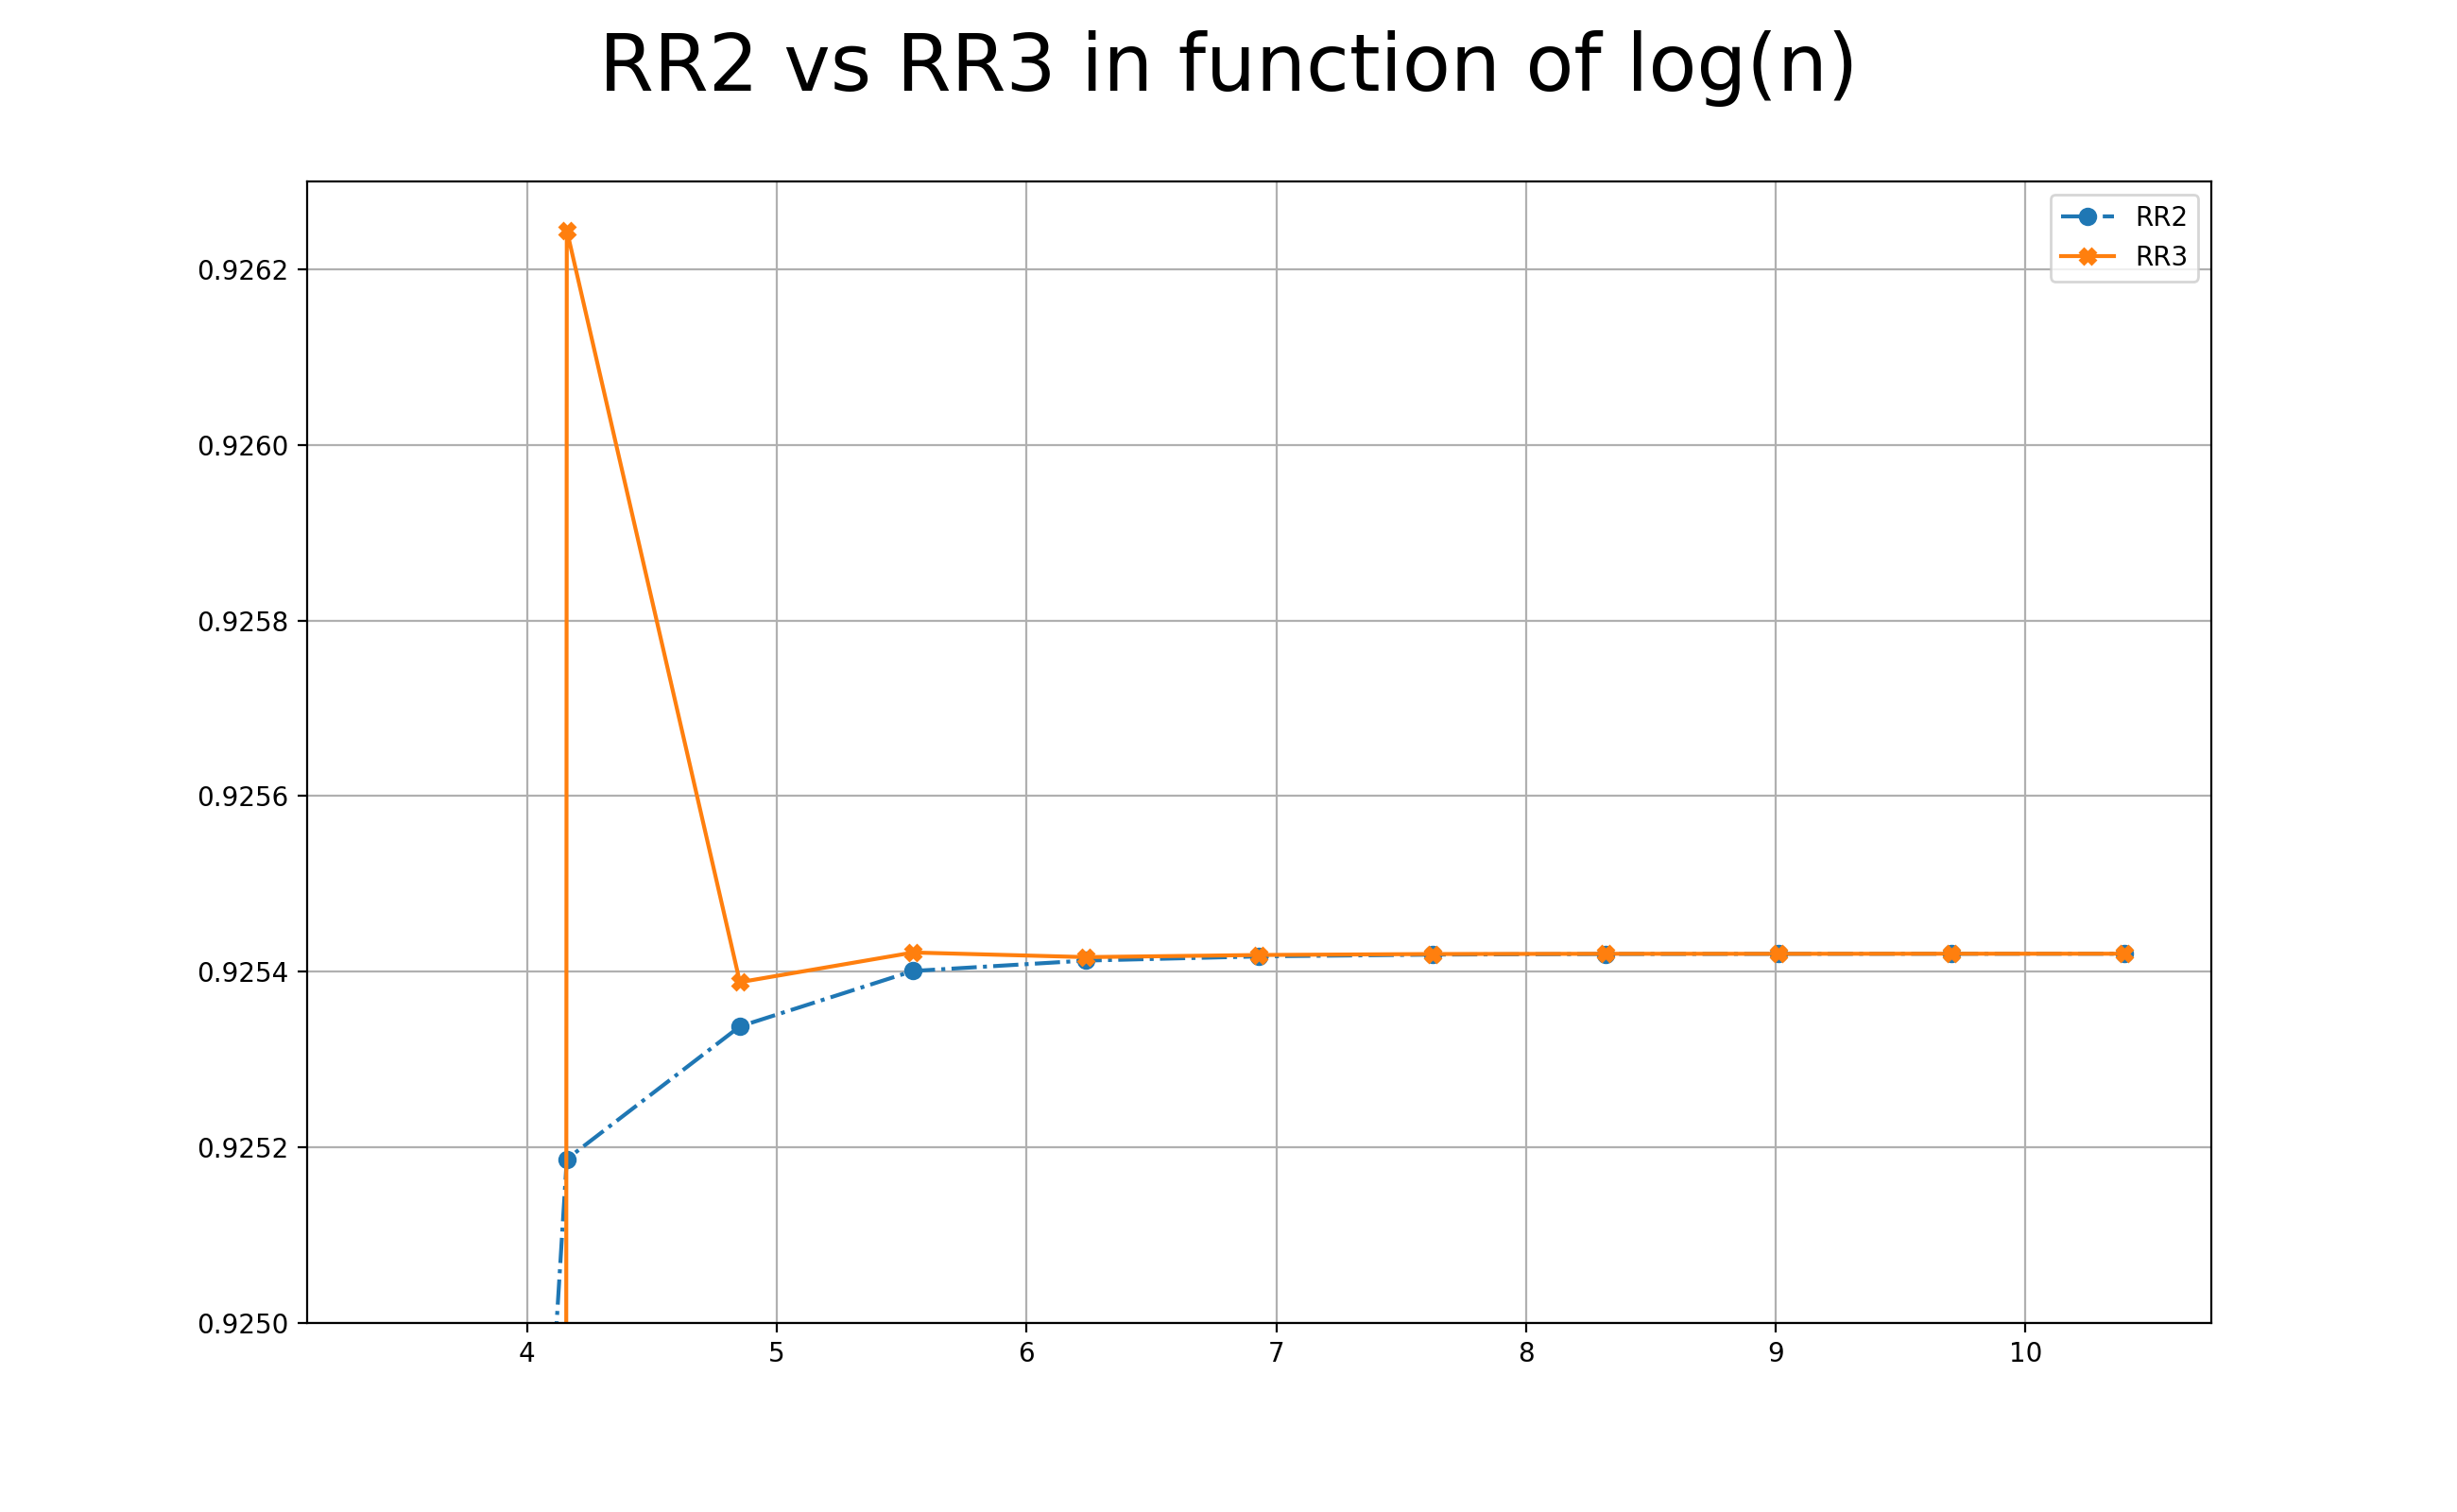
\includegraphics[width=\textwidth, height=60mm]{coefficients_test_2/extrapolatedrr_fine.png}
  \caption{same curves as of Figure \ref{comparisonComExtr2} zoomed on the $y$-axis. $RR2$ vs $RR3$: the red and blue lines are $\bar{\psi}^n_{RR,3}(T)$ and $\bar{\psi}^n_{RR,2}(T)$, respectively, as functions of $\log(n)$.
  This comes from the test with parameters \eqref{eq: NumericalTestParameters2}. }\label{comparisonComExtr2_fine}
\end{figure}

Summarising, many of the behaviours observed in the test with the parameters, \eqref{eq: NumericalTestParameters} are also observed with the parameters \eqref{eq: NumericalTestParameters2}. 
This is also true for other experimentations, whose results we do not report, where $\alpha$ is such that it produces the rough behaviour of the fractional Brownian motion ($\alpha < \frac{1}{2}$). 
However, changing the signs of $\lambda, \mu, \nu$ might lead to slightly different results, but the consistency of the hybrid Euler scheme is mantained.


\chapter{Other Plus final comments}



\textcolor{red}{ What is left to do? precedentemente non abbiamo parlato dei tempi compitazionali di psi n. Per poi confrontare con machine learning forse. dove n può essere il numero di neuroni. }

\section{Forse aggiungerà la parte di machine learning se andrò in russia.}

\section{Commenti finali}


\subsection{Cose tralasciate}

\textcolor{red}{Cose che ho saltato}. Salta la dimostrazione del teorema lungo sul raggio di convergenza. Poi salta anche la parte sul remainder term. Dove si stima di quanto si sbaglia troncando. Scrivi i risultati, ma senza dimostrazione. \\
Inoltre, per gli altri metodi, non serve che metta come si ricava la tripletta. A noi interessa solo psi. Se scrivi troppo poco posso compensare parlando della discretizzazione di Eulero.





\begin{thebibliography}{}

\bibitem{fBmExistence} Rogers, L.C.G. and Williams, D.: Diffusions, Markov Processes, and Martin-
gales, Volume 1: Foundations. Cambridge University Press, 2000.

\bibitem{ZhangBook} Biagini F., Hu Yaozhong, Zhang Tusheng, 
Øksendal Bernt,
\textit{Stochastic Calculus
for Fractional Brownian
Motion and Applications}, Springer 2006 

\bibitem{Omar} El Euch, O. and Rosenbaum, \textit{The characteristic function of rough Heston models.}. Mathe-
matical Finance, 29(1):3–38, M. (2019)

\bibitem{libro19} Samko, S., Kilbas, A., and Marichev. \textit{Fractional integrals and derivatives. Theory and
Applications}, Gordon and Breach, Yverdon, O. (1993).

\bibitem{Main} Callegaro G., Grasselli M., Pagès G. \textit{Fast Hybrid Schemes for Fractional Riccati Equations
(Rough is not so Tough)}, Mathematics of Operations Research, Vol. 46, 221-254, 2021

\bibitem{StevenGaussian} Lalley P. Steven. \textit{Introduction To Gaussian Processes.} https://galton.uchicago.edu/~lalley/Courses/386/GaussianProcesses.pdf

\bibitem{156!} Maslowski B., Nualart D. \textit{Evolution equations driven by a fractional
Brownian motion.} Journal of Functional Analysis, 277–305, 2003.

\bibitem{NourdinIvan} Nourdin Ivan. \textit{Selected aspects of fractional Brownian motion}, Bocconi Springer, 2004.

\bibitem{lemma11.1} Kallenberg O. \textit{Foundations of modern probability.} Springer, 1997

\bibitem{wikipediaMertens} Rudin W. \textit{Principles of Mathematical Analysis}, McGraw-Hill, 3rd edition, 1976

\bibitem{normalRiccati} Heston L. S., \textit{A closed-form solution for options with stochastic volatility with applica-
tions to bond and currency options.}, Review of Financial Studies. 327–343, 1993.

\bibitem{rosenbaum1} Gatheral J., Jaisson T., Rosenbaum M. (2018). \textit{Volatility is rough}. Quantitative Finance, 18(6):933–
949.

\bibitem{wikipediaCauchy} \textit{Cauchy formula for repeated integration}, Wikipedia.

\bibitem{nemesGamma} Nemes G., \textit{New asymptotic expansion for the gamma function.} Archiv der Mathematik (Springer Basel) 95, 161-169 (2010)

\bibitem{RR3extr} Pagès G. \textit{Multi-step Richardson-Romberg extrapolation: remarks on variance control and
complexity.} Monte Carlo Methods and Applications Journal, 13(1):37–70 (2007).

\end{thebibliography}

\appendix 

\chapter{Python Code: Hybrid Euler Scheme}
\label{appendix: hybridEulerScheme}

\section{Computing $\left\{ \bar{\psi}^n\right\}_{n\in \mathbb{N}}$.}
\noindent
\textbf{Step 1.}

\begin{lstlisting}
alpha = 0.64
lambd = 0.045
mu = -64.938
nu = 44850

# error measures
epsilon = 0.01
theta = 0.9

r_max = 105
T = 1/252
\end{lstlisting}
\\
\\
\textbf{Step 2.}

\begin{lstlisting}
import pandas as pd
import numpy as np
import math

def returns_all_the_first_r_max_coefficients_as_list_2():
    ''' Run this function. This returns the list of coefficients. 
    Up to a_k where k = r_max. '''
    
    coefficients = [np.nan]*(r_max+1)

    a0 = 0 
    a1 = nu/math.gamma(alpha+1)
    coefficients[0] = a0
    coefficients[1] = a1
    
    def recursive_convol_coefficients(list_of_coefficients, k):
        ''' return a*_k^2  given the first k-1 a_m coefficients. 
        k is the coefficient a^_k^2 to be returned'''
        if k==1:
            return 0
        else: 
            sum = 0
            for l in range(1,k):
                a_l = list_of_coefficients[l]
                a_k_l = list_of_coefficients[k-l]
                sum += a_l*a_k_l
            return sum
    
    def recursive_coefficients(list_of_coefficients, n):
        ''' Given the convoluted coefficient a_k_star_quadro, 
        Given also n, the coefficient a_n to be returned.
        Note that n = k+1 !!! 
        returns a_k'''
        
        k = n-1  #n-1 = k
        a_k_star_quadro = recursive_convol_coefficients(
                            list_of_coefficients, k) 
        a_k = list_of_coefficients[k]  
        a_n = (lambd*a_k_star_quadro + mu*a_k)*math.gamma(alpha*k+1)
                /math.gamma(alpha*k+alpha+1)
    
        return a_n

    for i in range(2, r_max+1):
        coefficients[i] = recursive_coefficients( coefficients, i)
        
    return coefficients
    
    coeff = returns_all_the_first_r_max_coefficients_as_list_2()
\end{lstlisting}
\\

\noindent
\textbf{Step 3.}
\begin{lstlisting}
a_r_max = coeff[-1]
a_primo_r_max = a_r_max*math.gamma(alpha*r_max+1)
               /math.gamma(alpha*r_max-alpha+1)
               /(alpha*r_max+1-alpha)

R_estimate = abs(a_primo_r_max)**(-1/(alpha*r_max))
\end{lstlisting}

\\
\\
\\
\noindent
\textbf{Step 4.}
\begin{lstlisting}

r_0 = math.log(epsilon*(1-theta))/alpha/math.log(theta)-1
r_0 = int(np.round(r_0)+1)

\end{lstlisting}

\\
\noindent
\textbf{Step 5.}
\begin{lstlisting}
def poly(lst, x):   
    ''' Evaluate the polynomial with coefficients lst= [a0,a1,a2,...] 
    in x.
    Pol: a0 + a1*x**alpha + a2*x**(2*alpha) + .... '''
    n, tmp = 0, 0
    for a in lst:
        tmp = tmp + (a * (x**(n*alpha)))
        n += 1

    return tmp

def computing_psi_n(n):
    
    disc_times = [k*T/n for k in range(0,n+1)]
    
    k_0 = math.floor(R_estimate*theta*n/T)  
    t_k_0 = disc_times[k_0]
    
    values_assumed_in_disc_times = [np.nan]*(n+1)
    
    ### Here We Evaluate The Truncated Series!
    for k in range(0,k_0+1):
        values_assumed_in_disc_times[k]=poly(coeff_truncated, disc_times[k])
    
    
    ### Here Instead We Use The Euler Scheme
    def compute_c_i(alpha, l):
        if l == 0:
            return 1
        else: 
            return (l+1)**alpha - l**alpha
            
    
    for k in range(k_0+1, n+1):
        factor_1 = 1/math.gamma(alpha + 1)*(T/n)**alpha
        addend_2 = nu*k**alpha 
        addend_3 = 0
        for l in range(1,k):
            psi_n_t_l = values_assumed_in_disc_times[l]
            addend_3 += compute_c_i(alpha, k-l-1)
                     *psi_n_t_l*(lambd*psi_n_t_l + mu)
        
        factor_2 = addend_2 + addend_3
        result = factor_1*factor_2
        values_assumed_in_disc_times[k] = result
            
    #return disc_times, values_assumed_in_disc_times
    return pd.DataFrame({"time": disc_times, 
             "value": values_assumed_in_disc_times}), t_k_0
\end{lstlisting}

\section{Computing $\left\{ \bar{c_1}^n \right\}_{n\in \mathbb{N}}$.}

\noindent
\textbf{Definition of the sequence $\left\{ \bar{c_1}^n \right\}_{n\in \mathbb{N}}$.}

\begin{lstlisting}
def c_1(n):
    return (2*n*(computing_psi_n(n)[0].iloc[-1].value - 
       computing_psi_n(2*n)[0].iloc[-1].value))
\end{lstlisting}

\noindent
\textbf{Computational times.}

\begin{lstlisting}
import time

df_ci_times = {} 
df_ci_values = {}

for i in [2**k for k in range(2,14)]:
   start_time = time.time()
   df_ci_values[i] = c_1(i)
   df_ci_times[i] = time.time() - start_time
   
final = pd.DataFrame({"n": [key for key in df_ci_times], 
   "c_n": [df_ci_values[key] for key in df_ci_values], 
   "comput_time -sec-": [df_ci_times[key] for key in df_ci_times]})

final = final.set_index("n")

final['comput_time_rapport'] = (final['comput_time -sec-']/
   final['comput_time -sec-'].shift(1))

print(final)
\end{lstlisting}

\section{Richardson-Romberg's estimates.}

\noindent
\textbf{Definition of the Richardson-Romberg's estimates.}

\begin{lstlisting}
def richardson_romb_2(n) :
    if n%2 == 0:
        return (2*computing_psi_n(n)[0].iloc[-1].value -     
           computing_psi_n(int(n/2))[0].iloc[-1].value)
    else:
        print('Error. Insert n even')
        
def richardson_romb_3(n):
    if n%4 == 0:
        addend_1 = 1/3*computing_psi_n(int(n/4))[0].iloc[-1].value
        addend_2 = -2*computing_psi_n(int(n/2))[0].iloc[-1].value
        addend_3 = 8/3*computing_psi_n(n)[0].iloc[-1].value
        return addend_1+addend_2+addend_3
    else:
        print('error. Insert n multiple of 4')
\end{lstlisting}

\noindent
\textbf{Computational times.}


\begin{lstlisting}
rr2 = {}
compt_time_2 = {}
rr3 = {}
compt_time_3 = {}

import time

for n in [2**k for k in range(5,16)]:
    start_time_2 = time.time()
    rr2[n] = richardson_romb_2(n)
    compt_time_2[n] = time.time()-start_time_2
    
    start_time_3 = time.time()
    rr3[n] = richardson_romb_3(n)
    compt_time_3[n] = time.time()-start_time_3

fin_extr = pd.DataFrame({"n": [key for key in rr2], 
    "rr2": [rr2[key] for key in rr2], 
    "rr3": [rr3[key] for key in rr3], 
    "comp2" : [compt_time_2[key] for key in rr2], 
    "comp3":  [compt_time_3[key] for key in rr2]})

print(fin_extr)
\end{lstlisting}





\chapter{Python Code: Machine Learning Parts}

\section{First Neural Networks}

\section{Others}



\end{document}
